\title{農業におけるWikiを活用する知の構造化}
\author{プロジェクトマネジメントコース\\
ソフトウェア開発管理グループ\\
矢吹研究室\\
1242034\\
小池 克人}
\date{}
\begin{document}
\maketitle

%本テンプレートの余白は,卒論マニュアルで指示されたものとは違っているが,1ページあたりの文字数は40文字x40行と,卒論マニュアル通りになっている。文字間隔や行間隔を調整して,余白をマニュアル通りにすることもできるが,それでは文章が読みにくくなるため,このような対応をしている。

%\noindent
□□□□□□□□□■□□□□□□□□□■□□□□□□□□□■□□□□□□□□□■
□□□□□□□□□■□□□□□□□□□■□□□□□□□□□■□□□□□□□□□■
□□□□□□□□□■□□□□□□□□□■□□□□□□□□□■□□□□□□□□□■
□□□□□□□□□■□□□□□□□□□■□□□□□□□□□■□□□□□□□□□■
□□□□□□□□□■□□□□□□□□□■□□□□□□□□□■□□□□□□□□□■
□□□□□□□□□■□□□□□□□□□■□□□□□□□□□■□□□□□□□□□■
□□□□□□□□□■□□□□□□□□□■□□□□□□□□□■□□□□□□□□□■
□□□□□□□□□■□□□□□□□□□■□□□□□□□□□■□□□□□□□□□■
□□□□□□□□□■□□□□□□□□□■□□□□□□□□□■□□□□□□□□□■
□□□□□□□□□■□□□□□□□□□■□□□□□□□□□■□□□□□□□□□■
□□□□□□□□□■□□□□□□□□□■□□□□□□□□□■□□□□□□□□□■
□□□□□□□□□■□□□□□□□□□■□□□□□□□□□■□□□□□□□□□■
□□□□□□□□□■□□□□□□□□□■□□□□□□□□□■□□□□□□□□□■
□□□□□□□□□■□□□□□□□□□■□□□□□□□□□■□□□□□□□□□■
□□□□□□□□□■□□□□□□□□□■□□□□□□□□□■□□□□□□□□□■
□□□□□□□□□■□□□□□□□□□■□□□□□□□□□■□□□□□□□□□■
□□□□□□□□□■□□□□□□□□□■□□□□□□□□□■□□□□□□□□□■
□□□□□□□□□■□□□□□□□□□■□□□□□□□□□■□□□□□□□□□■
□□□□□□□□□■□□□□□□□□□■□□□□□□□□□■□□□□□□□□□■
□□□□□□□□□■□□□□□□□□□■□□□□□□□□□■□□□□□□□□□■
□□□□□□□□□■□□□□□□□□□■□□□□□□□□□■□□□□□□□□□■
□□□□□□□□□■□□□□□□□□□■□□□□□□□□□■□□□□□□□□□■
□□□□□□□□□■□□□□□□□□□■□□□□□□□□□■□□□□□□□□□■
□□□□□□□□□■□□□□□□□□□■□□□□□□□□□■□□□□□□□□□■
□□□□□□□□□■□□□□□□□□□■□□□□□□□□□■□□□□□□□□□■
□□□□□□□□□■□□□□□□□□□■□□□□□□□□□■□□□□□□□□□■
□□□□□□□□□■□□□□□□□□□■□□□□□□□□□■□□□□□□□□□■
□□□□□□□□□■□□□□□□□□□■□□□□□□□□□■□□□□□□□□□■
□□□□□□□□□■□□□□□□□□□■□□□□□□□□□■□□□□□□□□□■
□□□□□□□□□■□□□□□□□□□■□□□□□□□□□■□□□□□□□□□■
□□□□□□□□□■□□□□□□□□□■□□□□□□□□□■□□□□□□□□□■
□□□□□□□□□■□□□□□□□□□■□□□□□□□□□■□□□□□□□□□■
□□□□□□□□□■□□□□□□□□□■□□□□□□□□□■□□□□□□□□□■
□□□□□□□□□■□□□□□□□□□■□□□□□□□□□■□□□□□□□□□■
□□□□□□□□□■□□□□□□□□□■□□□□□□□□□■□□□□□□□□□■
□□□□□□□□□■□□□□□□□□□■□□□□□□□□□■□□□□□□□□□■
□□□□□□□□□■□□□□□□□□□■□□□□□□□□□■□□□□□□□□□■
□□□□□□□□□■□□□□□□□□□■□□□□□□□□□■□□□□□□□□□■
□□□□□□□□□■□□□□□□□□□■□□□□□□□□□■□□□□□□□□□■
■■■■■■■■■■■■■■■■■■■■■■■■■■■■■■■■■■■■■■■■
□□□□□□□□□■□□□□□□□□□■□□□□□□□□□■□□□□□□□□□■%文字数チェック用

 \chapter*{謝辞}
本研究を進めるに当たり,ご指導を頂いた卒業論文指導教員の矢吹太朗準教授に感謝致 します.また,矢吹研究室の同期や後輩のご協力に感謝します.
\tableofcontents%目次

 \chapter{序論}
本研究の目的は,Mediawikiを用いた翻訳システムの開発が目的である.農業では,研究,行政,流通,農家により作物名称が変わる.例を上げるとイチゴでもあまおうやゆめのかなど品種改良を行いイチゴではなく別の名称を生産者が付けた作物が作物ごとにいくつもある.さらに行政などで統計を取るときにもいちごやイチゴなど変わる.

そこで本研究では,様々な名称がある作物を用途に応じた翻訳システムの開発を目指す.統計を目的にした場合は,統計に適した語彙,研究を目的にした場合は,研究に適した語彙への翻訳・置き換えることをできるシステムを目指す.

Mediawikiを使い•上位下位関係抽出ツールで表示させる.そうすることで農業生産者が自分で農作物の情報をMediawikiに書き込ことができる.生産者が書き込んだ情報を上位下位関係抽出ツールで用途による語彙への変換ができると考える.


 \chapter{背景}
平成27年3月10日に発表された農業情報の標準化に関する個別ガイドラインでは,農業の情報の相互運用性を確保するインターオペラビティーとポータビリティー確保の標準化が必要とされている\cite{naikaku2014}.

しかし,異なる企業や団体の意思を一つにまとめる作業には困難が伴う.標準化して,データをやり取りするプロトコルやデータ形式は各企業の利害がぶつかるため,困難である\cite{kizi2015}.よって,複数のシステムの間でマスターを統一しようとする共通語彙には,目的と実現する考え方のアーキテクチャーが異なり,マスターは構造も用語も異なるため現実感が無いため,共通的な方法論ができないかを考える.

作物名称は,研究,行政,流通,農家により変わる.研究は研究目的に応じた分類のため,行政は行政の目的に応じた分類のため,流通は流通に都合の良いネーミングのため,農家は営農の都合に良い分類のための用途により視点が異なる.よって,以下の図のように用語も異なる.

\begin{table}[htb]
  \begin{center}
  \begin{tabular}{|l|c|r|r|} \hline
    作物名 & 代表名 & 種別 & 出荷統計作物名 \\ \hline \hline
    あまおとめ & イチゴ & 果菜類 & いちご \\  \hline
    ゆめのか & イチゴ & 果菜類 & いちご \\  \hline
    サクサク王子 & インゲン & 果菜類 & さやいんげん \\  \hline
    まくわ & ウリ & 果菜類 & うり類 \\  \hline
    おつなひめ & エダマメ & 果菜類 & えだまめ \\  \hline
    キヌサヤ & エンドウ & 果菜類 & さやえんどう \\  \hline
    グリーンマロー & カボチャ & 果菜類 & かぼちゃ \\  \hline
   Jきゅうり & キュウリ & 果菜類 & きゅうり \\  \hline
  \end{tabular}
  \end{center}
\caption{様々な作物表}
\end{table}

今回の研究では,異なる作物名称を目的に応じた用語に変換(翻訳)するための,共通する仕組みがないかということに着目した.用語の変換をするために用語を上位下位で結び,関連用語を抽出することを考える.関連用語の抽出をしている事例を探し,参考にして研究する.そして.2008年のWikipediaの記事構造からの上位下位関係抽出の論文を参考にして,MediaWikiを利用する\cite{nogyo2015}.MediaWikiは,オープンソース(GPL)で配布されているため,MediaWikiを用いれば,自分専用のWikipediaを設置・運用することができる\cite{nico2015}.MediaWikiを利用し,目的に応じて最適な語彙の翻訳を可能とする翻訳システムの開発を研究する.


\chapter{目的}
様々な品種や用途で呼び方の変わる農作物を研究,行政,流通,農家などの農業情報の用途や目的により視点,用語が異なる語彙を目的に応じた最適な語彙への翻訳ができるような仕組みを作ることが目的である.

\chapter{プロジェクトマネジメントとの関連}
本研究は,仕様書や設計書などのドキュメントを作成する時に意味が同じであり,単語が複数ある語彙を統一して十分に理解するために使用する.

これは発注者と開発者の不適切なコミュニケーションを避けることが出来るため,プロジェクト情報の計画,収集,生成,配布,保管,検索,マネジメント,コントロール,監視,そして最終的な廃棄を適時かつ適切な形で確実に行うために必要なプロセスからなる.

そのことからコミュニケーションマネジメントに関連すると考えられる.

\chapter{農業について}
\section{本章の構成}
本章では,研究対象である農業について解説する.また,農業にに関連する事項も記す.
\section{農業とは}
農業とは,土地を利用して作物の栽培または家畜の飼養を行い,人間にとって有用な生産物を生産する経済活動であり,そのような活動を行う産業である.人間に有用な農業生産物は食糧と一部の工業原料であるが,農業はそれらを,土,水,太陽エネルギーなどの自然力を利用して作物として生産し,また家畜を繁殖,肥育させることによってそれを生産する.このような農業の産業としての特質は,第1に,土地を基本的な生産手段とし,またその土地を商工業などの他産業と比較して,広い面積にわたって相対的に粗放に利用することであり,第2に,人間が長い年月をかけて育成し,または馴らしてきた高等動植物を対象(もしくは手段)とする,有機的生産であることである.\cite{nouwiki2015}
\section{農業の種類}
主な農業の種類を解説する.\cite{kotoba}

\subsection{地中海式農業}
地中海式気候の地域に独特な農業様式のことである.地中海沿岸が代表的で,夏季の高温乾燥に耐えるブドウ,オリーブ,オレンジなどの果樹栽培(おもに丘陵地斜面),冬雨を利用する平地でのコムギ栽培,家畜飼育(ヒツジ,ヤギなど)を組み合わせた農業.
\subsection{酪農}
乳牛を飼育して牛乳および乳製品の生産を行う農業経営.近代的酪農は,早くから有畜の輪栽式農法を行い,畜産物を日常の食品としていたヨーロッパで農業革命後に発展した.

\subsection{園芸農業}
都市への出荷を目的として野菜,果樹,花卉,花木,緑化樹木などを栽培する集約的農業.都市近郊に発達する近郊農業,都市から離れたところに発達する輸送農業などがあり,栽培方法には露地栽培,促成栽培,抑制栽培などがあるが,いずれも都市市場の価格と見合う栽培方法をとっている.

\subsection{混合農業}
種と家畜の飼育を有機的に結びつけた農業.耕種部門では穀物より飼料作物に重点がおかれ,小麦,ライ麦,大麦,じゃがいも,とうもろこしなどを科学的に輪作する.家畜は牛,豚,羊などが多い.
\subsection{プランテーション農業}
熱帯,亜熱帯で行なわれる栽植農業.欧米人が資本,技術を提供し,熱帯の労働に耐え得る先住民や移入労働者の安価な労働力を利用して,モノカルチャー経済を行なう企業的農業経営のこと.作物は貿易品として価値のある香料作物,ゴム,チャ (茶) ,麻,キナノキ,コーヒー,カカオ,サトウキビ,バナナ,タバコなどがある.
\section{品種改良とは}
品種改良とは,生物の遺伝質を人工的に変えて,一段と利用価値の高い新しい型のものを作り出すこと.新しい地域に従来なかった新種,新品種を導入することや,全く新しい生物種を創出することも含む.\cite{kinoko2015}
\section{方法}
主な方法は,別の品種と別の品種を掛け合わせて別の品種を作り,繁殖させる方法が主な方法である.

いろいろな性質のものの中から目的に合ったものを選び出すことで,様々な性質のものが作り出される.

%図の挿入
\begin{figure}[htb]
\centering
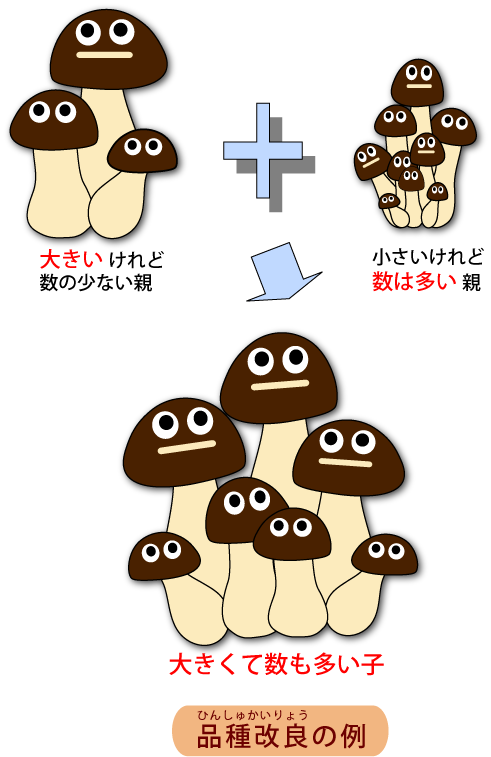
\includegraphics[width=5cm]{kinoko8.png}
\caption{品種改良の例}\label{図}
\end{figure}

\section{遺伝子組み換えとは}
遺伝子組み換えとは,人為的に遺伝子工学の手法を用いて試験管内で遺伝子を組み換えることである.

遺伝子組み換えをGMO,遺伝子組み換えをしない通常のものをnon-GMOと呼ぶ.\cite{kinoko2015}

%図の挿入
\begin{figure}[htb]
\centering
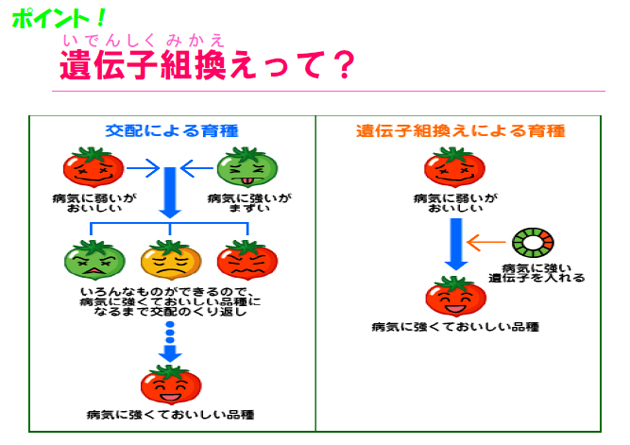
\includegraphics[width=10cm]{iden.jpg}
\caption{遺伝子組み換え}\label{図}
\end{figure}

\subsection{遺伝子組み換えと品種改良の違い}
遺伝子組み換えと品種改良の違いは,人為的か自然に行われるかの違いである.遺伝子組み換えは,人為的に目的の遺伝子を処理するため特定の効果を得るが,品種改良は,自然交配による突然変異種を期待するものである

品種改良は,期待通りのものができるまでに年月がかかる.さらに,確立は,かなり低い\cite{idennsi}

\subsection{メリット}
遺伝子組み換えによるメリットは主に,除草剤に耐性と害虫に強くなることが挙げられる.この2つは,栽培するときに農薬をまく回数を減らすため,作業負担を軽減する.そのため,生産へのコストを下げることができる.
\subsection{デメリット}
%図の挿入
\begin{figure}[htb]
\centering
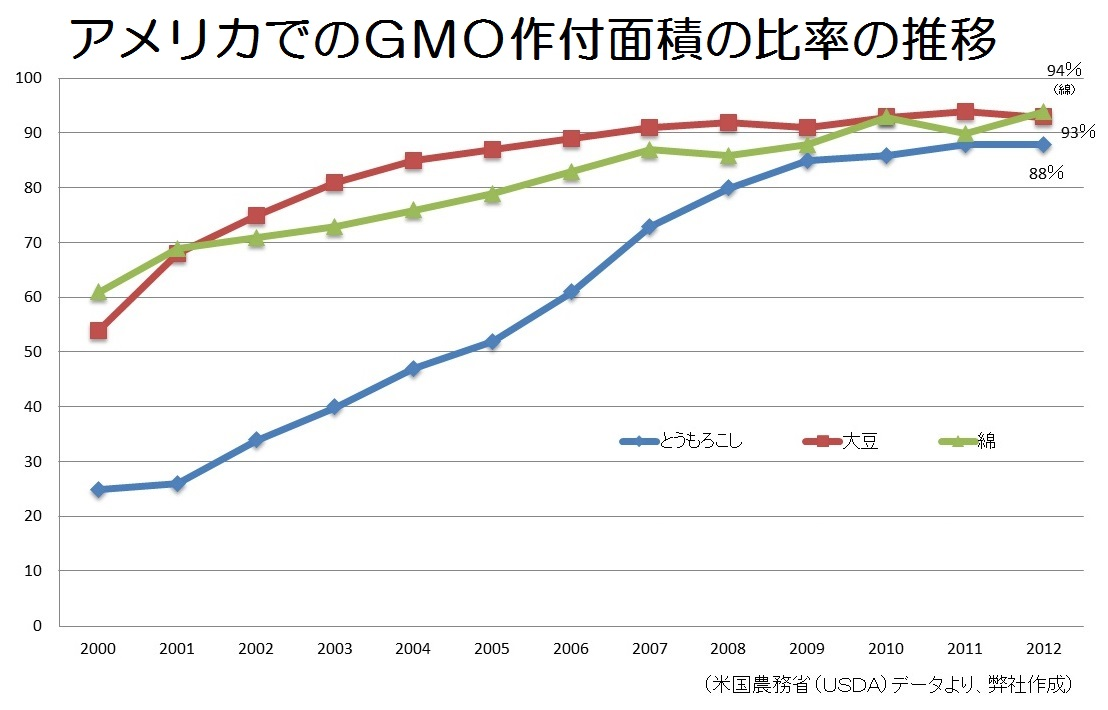
\includegraphics[width=10cm]{GMO.jpg}
\caption{GMO推移比率データ}\label{図}
\end{figure}

デメリットは,健康に健康に悪影響を与える可能性が高いことが挙げられる.アメリカでは,遺伝子組み換えで栽培されているトウモロコシと大豆の比率が高く約9割が遺伝子組み換えになっている.\cite{akikawa}

遺伝子組み換え食品の割合が多いアメリカでは,遺伝子組み換え食品の出現と共にガン,白血病,アレルギー,自閉症などの慢性疾患が急増しているというデータが出ている.このデータが遺伝子組み換えの有害性を断言できるわけではないが,可能性を指摘できる.\cite{mondsi}
%図の挿入
\begin{figure}[htb]
\centering
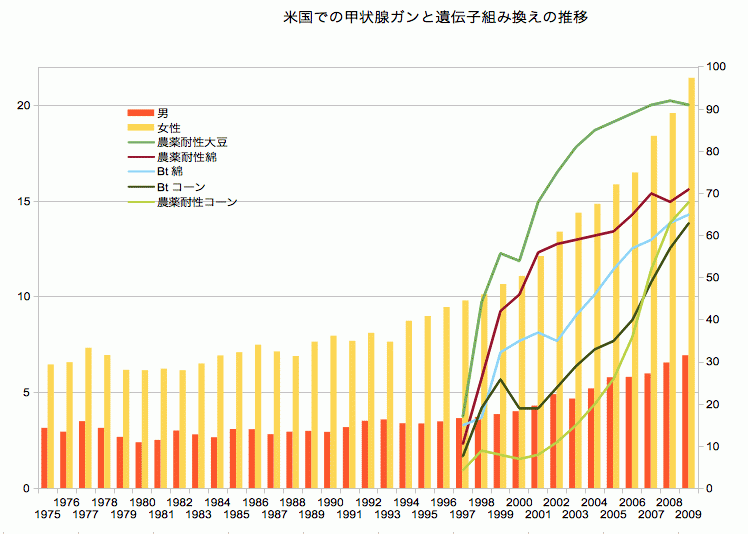
\includegraphics[width=10cm]{gan.png}
\caption{アメリカでの甲状腺ガンと遺伝子組み換えの推移}\label{図}
\end{figure}


\section{現在の農業情報}
現在の農業では,品種改良,遺伝子組み換えをした農作物が大量に存在する.苺で例えると,アイベリー,あかねっ娘,あきひめ,あまおう,あすかルビー,あまおとめ,あわゆき,えちごひめ,エラン,おおきみ,おいCべりーおとめごころ,かおりのと同じ苺でも大量に存在する.

 さらに農作物は,農家,流通,研究,行政によって名称が変わりる.農家は営農に都合の良いように,流通は都合の良いように産地名やブランド名などのために,研究は研究目的に応じた新品種開発や防疫,防虫のために,行政は行政の目的に応じた統計作りや分類のためによって用語や用途が変わる.

\chapter{Wikiについて}
\section{本章の構成}
本章では,研究の対象であるWikiについて基本知識と関連する 解説を記述する .
\section{Wikiとは}
Wikiとは,Webブラウザから簡単にWebページの発行・編集などを行えうことができる,Webコンテンツマネジメントシステム(CMS)の1つである.

複数人が共同でWebサイトを構築していく利用法を想定しており,閲覧者が簡単にページを修正や新しいページを追加することができるようになっている.編集者をパスワードなどで制限,編集できないよう凍結することもできる.HTMLの知識がなくてもリストやリンクを簡単に作成できるようになっており,簡易な整形書式が定められている.

Wikiは,内容の編集・削除が自由なこと,基本的に時系列での整理を行わないことから,誰もが自由に「記事」を書き加えていくコラボレーションツールに近い.柔軟性が高く,手軽に始められて操作が簡単なことから,特定のテーマのまとめサイトの制作に利用されることが多い.\cite{wiki}
\section{特徴}
主なWikiの特徴は3つ挙げられる.\cite{wiki3}
\begin{enumerate}
\item Web上であれば,場所や日時関係なく誰にでも文章を書き換えることができる.
\item 文章を書き換えるのにウェブブラウザのみでできる.
\item HTMLより簡単なマークアップ構文で書くことができる.
\end{enumerate}
\section{歴史}
Wikiのソフトウェアは,デザインパターンの共同体でパターン言語を書くために創られたものである.1995年にウォード・カニンガムが確立したPortland Pattern Repositoryが初のWikiだった.

カニンガムは,Wikiの概念を発明し名付け,Wikiエンジンの初の実装を製作した.元々のWikiだけが,Wikiあるいはウィキウィキウェブと呼ばれるべきだと主張する人もいる.カニンガムのウィキ (Wards Wiki) はいまだに最も人気のあるウィキサイトの1つである.

20世紀の最後の数年に,WIkiは非公開・公開のナレッジベース(知識の基地)を開発するのに有望な技術であるということが,ますます認知されるようになった.そしてこの潜在能力は, Nupedia という百科事典プロジェクトの開祖ジンボ・ウェールズ(Jimmy Donal "Jimbo" Wales)とラリー・サンガー(Lawrence Mark "Larry" Sanger)に,ウィキ技術を電子百科事典の基礎に使おうというひらめきを与えた.

このことからウィキペディアは,2001年の1月に始まった.初めはUseModソフトウェアを基にしていたが,後にいくつかの他のウィキから取り込まれた独自のオープンソースのコード基盤に切り替えられた.

今日においては,一番項目の多いWikiは英語版ウィキペディアといわれる.非英語のウィキペディアも世界でも比較的に大きい.しかし,2004年において世界で二番目に大きいウィキはUseModというソフトを使うスウェーデン語のSusning.nuであったように,ウィキペディア以外のウィキでも大きなウィキは存在する.\cite{wiki}
\section{活用例}
Wikiは,誰でも,ネットワーク上のどこからでも,文書の書き換えができるようになっているため,不特定多数の共同記事を作成することに向いている.

例えば技術ドキュメントや仕様書の作成,会議の議題や議事録の共有,開発部門やサポート部門の間でのナレッジ共有,事例や凡例の共有などの利用方法などが挙げられる.\cite{wikiwiki}

%図の挿入
\begin{figure}[htb]
\centering
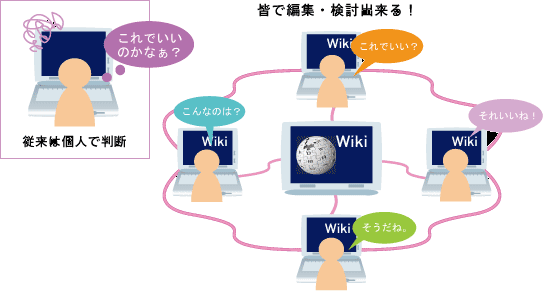
\includegraphics[width=10cm]{img_wiki03.png}
\caption{ウィキの活用例}\label{図}
\end{figure}




\chapter{Wikipediaについて}
\section{本章の構成}
本章では,Wikipediaについて記す.
\section{Wikipedia とは}
Wikipediaとは,2000年に立ち上げられた百科事典Wikimedia Foundation, Incが運営しているインターネット上の百科事典である.Wikipediaは,インターネット上のウェブサイトにアクセス可能な全ての人が自由に編集に参加できる.

使用言語は,288言語あり,世界各国の言語で記事を展開している.日本語の記事だけでも約980,000もあり,全ての記事の数は,約34,000,000記事がある.\cite{wikipedia}

%図の挿入
\begin{figure}[htb]
\centering
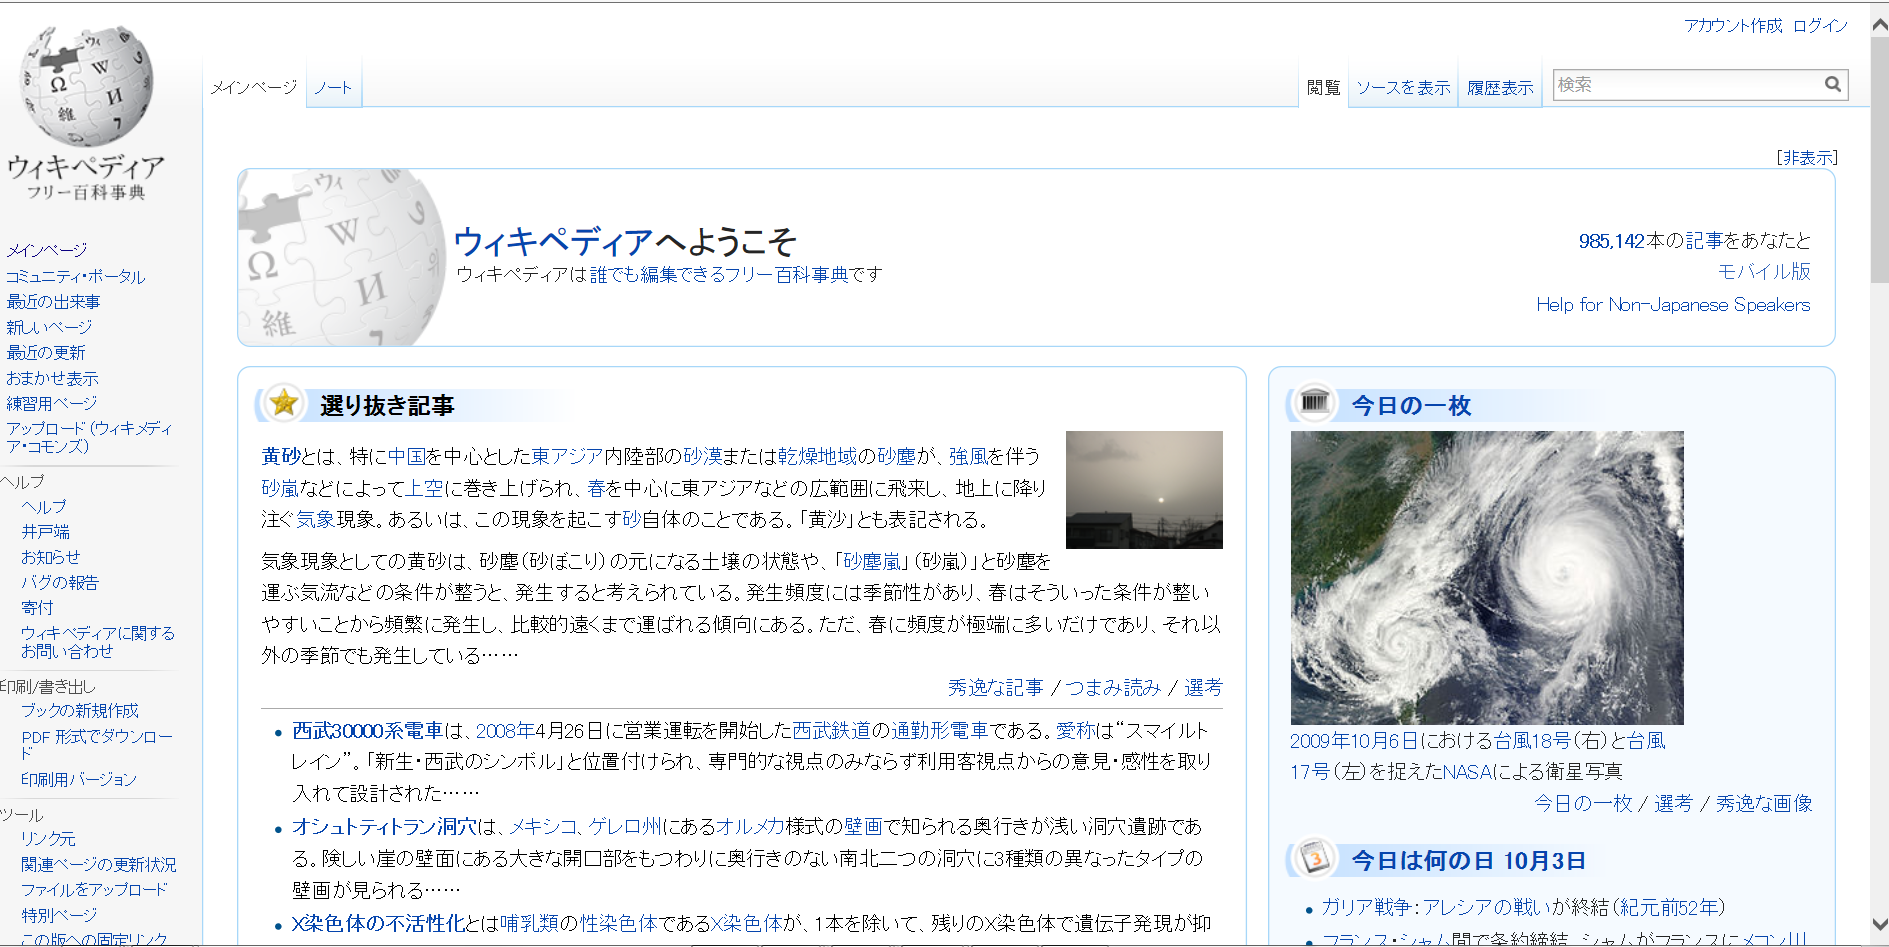
\includegraphics[width=12cm]{wikipedia.png}
\caption{wikipediaトップ画面}\label{図}
\end{figure}

\section{用語}
Wikipediaで主に使われている用語を解説する\cite{yougo}
\subsection{インターウィキリンク}
ウィキ間リンク,Interwikiとも.あらかじめ登録されている他のサイトへ簡便にリンクする方法.ウィキペディア内では,多言語版や姉妹プロジェクトへのリンクを張るのに使われる事が多く,その際に要約に「インターウィキ」 “interwiki“ などと記述される事が多い.
\subsection{ウィキ化}
既存の記事に対して,リンクなどのマークアップを行い,ウィキペディアの一般的なスタイルに整える作業.ウィキファイとも.初稿が文章のみの記述の場合に行われる事が多く,その際,要約欄には「wikify」や「ウィキ化」などと記述される場合が多い.

\subsection{ウィキプロジェクト}
特定の分野について統一的なフォーマットを用意し,ウィキペディア内でのスタイルの統一をはかる場.その分野の記事全体に関わる問題について,広く意見を求めるためにも利用される.
\subsection{ウィキポータル}
特定の分野の記事群に対して入り口となるポータルサイトを用意し,索引,更新情報,新規項目の依頼などその分野に関する情報を提供する場.
\subsection{管理者}
一般の利用者には制限されているいくつかの機能を行使でき,編集合戦や荒らしへの対策としてページを保護や問題のある利用者の投稿ブロックなどを行うことができる.ウィキペディアにおける発言の重みは一般利用者と同じものとされ,一般的に管理者という言葉がイメージさせるような大きな権限はない.
\subsection{サンドボックス}
試し書きや練習用として編集を実際に行なえるページ.一定時間が経つと,投稿した内容は消されるようになっている.ここ以外にも,編集の際に,プレビュー機能を使えばある程度だが代用できる.
\subsection{名前空間}
 端的に言えばウィキペディアの記事が属する分野のこと.ウィキペディアにおける記事名のうち,半角コロン (:) に先行する部分が名前空間名である.ウィキペディアには百科事典としての記事が置かれる通常名前空間やウィキペディア自身についての情報に関する記事が属するWikipedia名前空間のほかにも,利用者名前空間,Template名前空間などいくつかの名前空間がある.
\subsection{ボット}
ロボット(機械)の略語.自動的にウィキペディアの編集を行うプログラム.日本語版では,interlangの体裁を整えるボット,定型メッセージの形式を更新するボットなどが活動している.

\section{編集方法}

ウィキペディアの編集方法は,一部の保護されているページを除いて、全てのページには「編集」と書かれたリンクがありこのリンクをクリックする.


次に,クリックするとそのページのソースの書かれたページが開き,そのページに記述する.

記入し終わったら,編集内容の要約を記入し,「以上の記述を完全に理解し同意した上で投稿する」ボタンを押して保存する.
%図の挿入
\begin{figure}[htb]
\centering
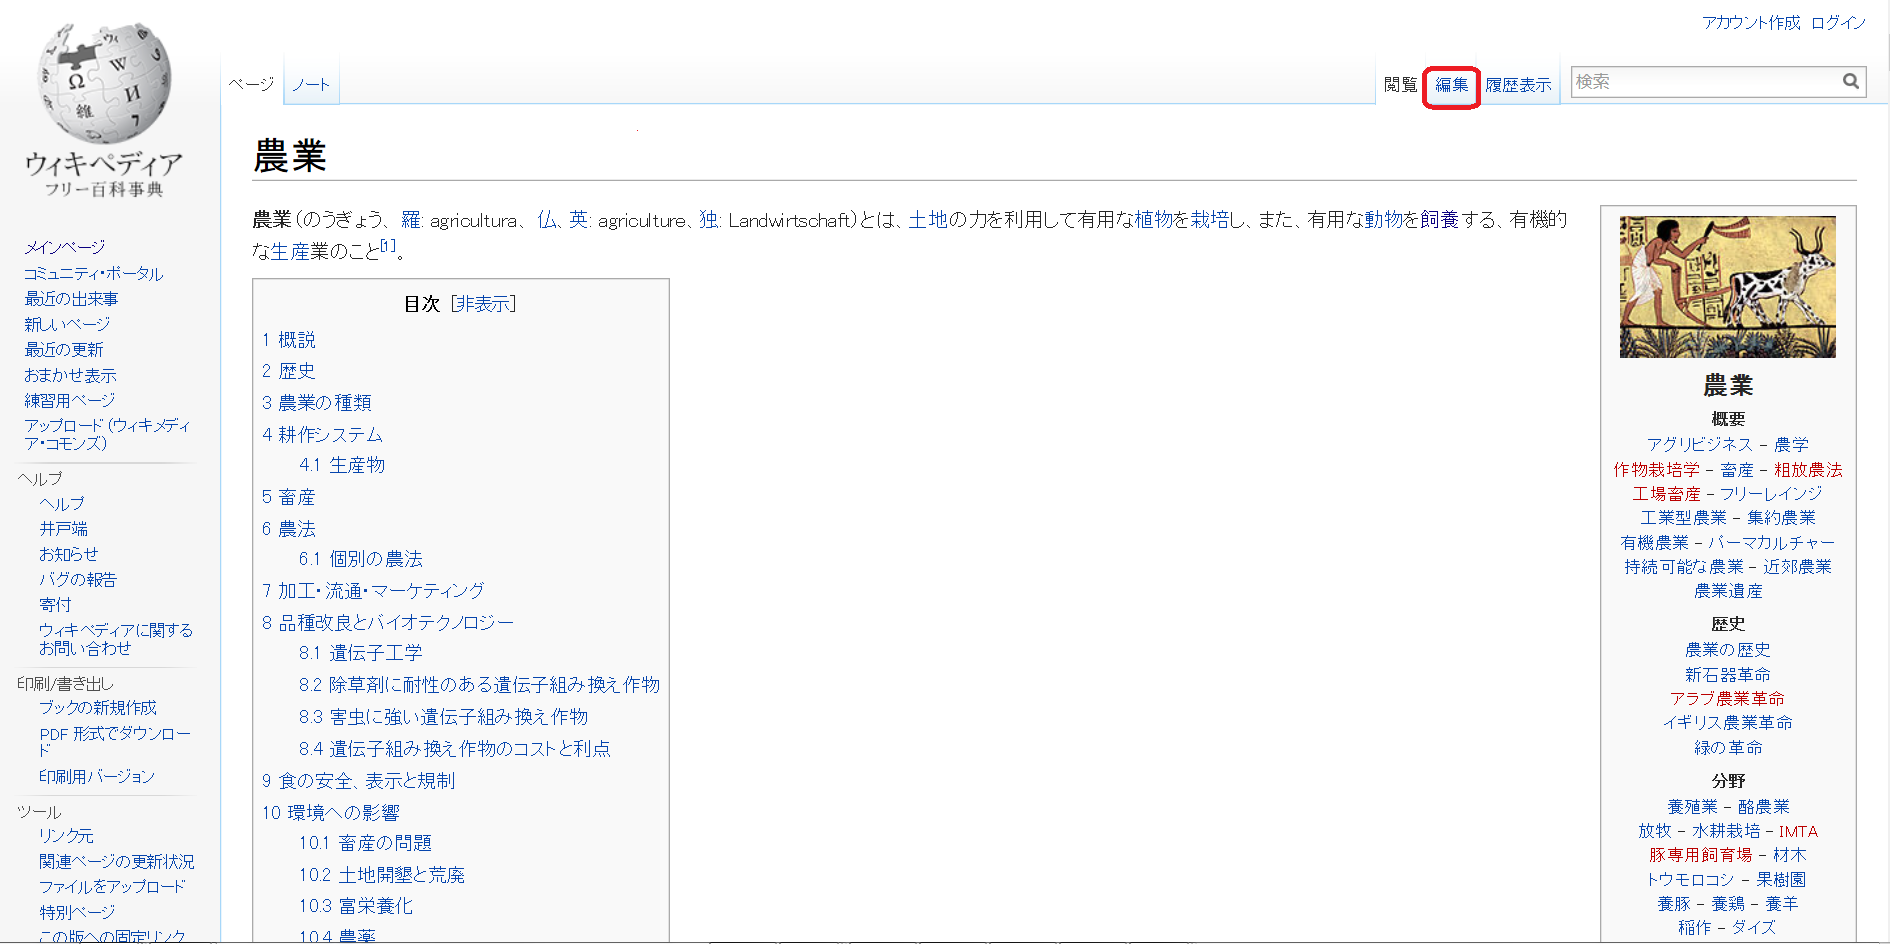
\includegraphics[width=15cm]{mudai.png}
\caption{編集画面1}\label{図}
\end{figure}

%図の挿入
\begin{figure}[htb]
\centering
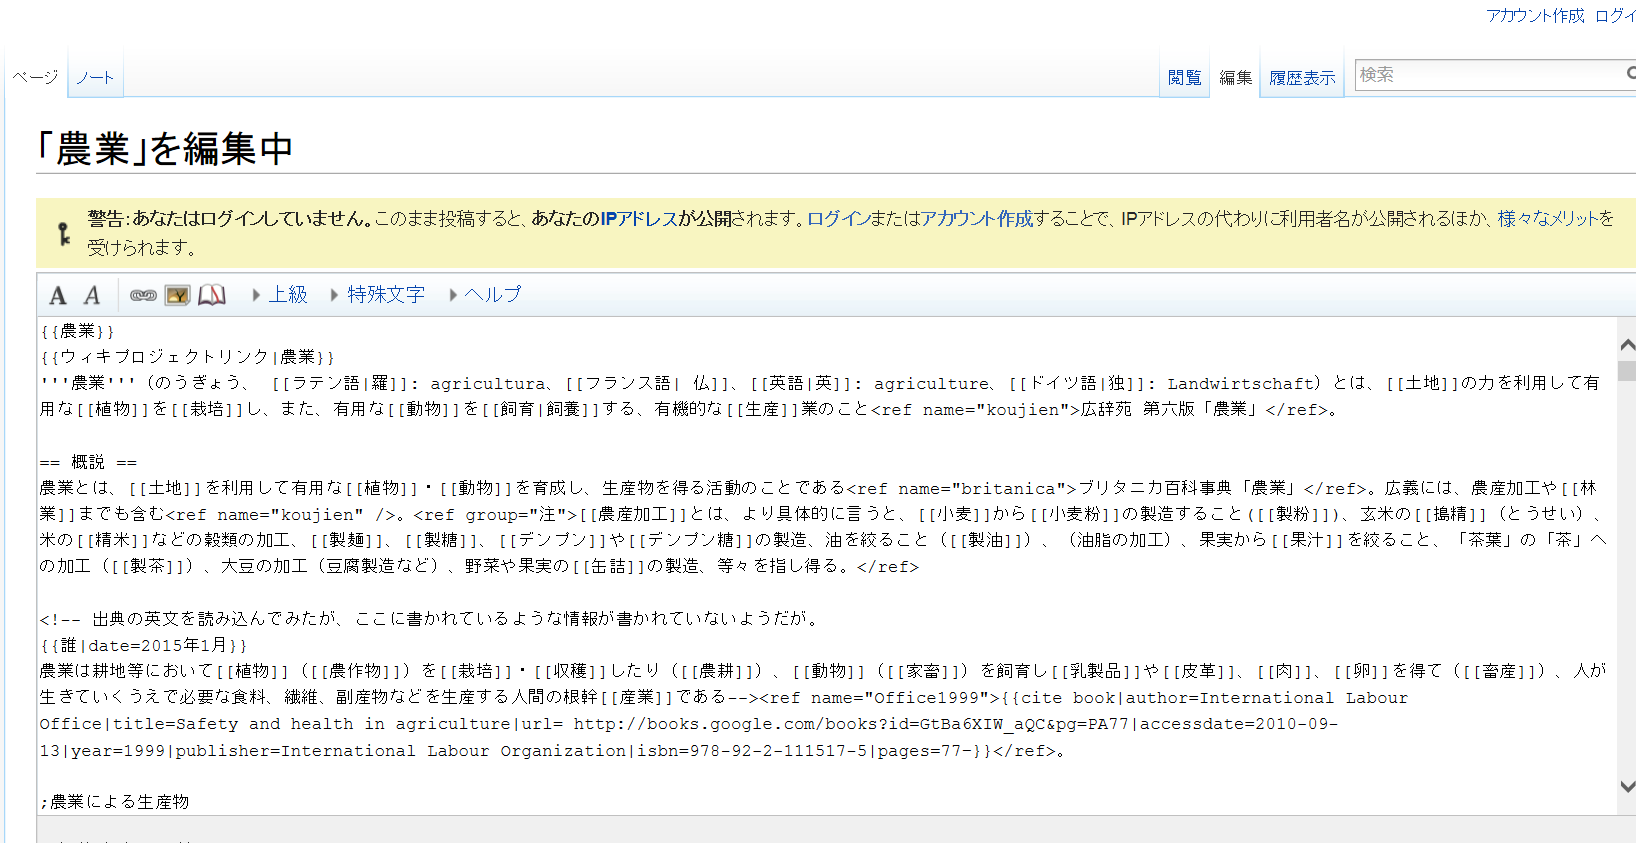
\includegraphics[width=15cm]{2.png}
\caption{編集画面2}\label{図}
\end{figure}

%図の挿入
\begin{figure}[htb]
\centering
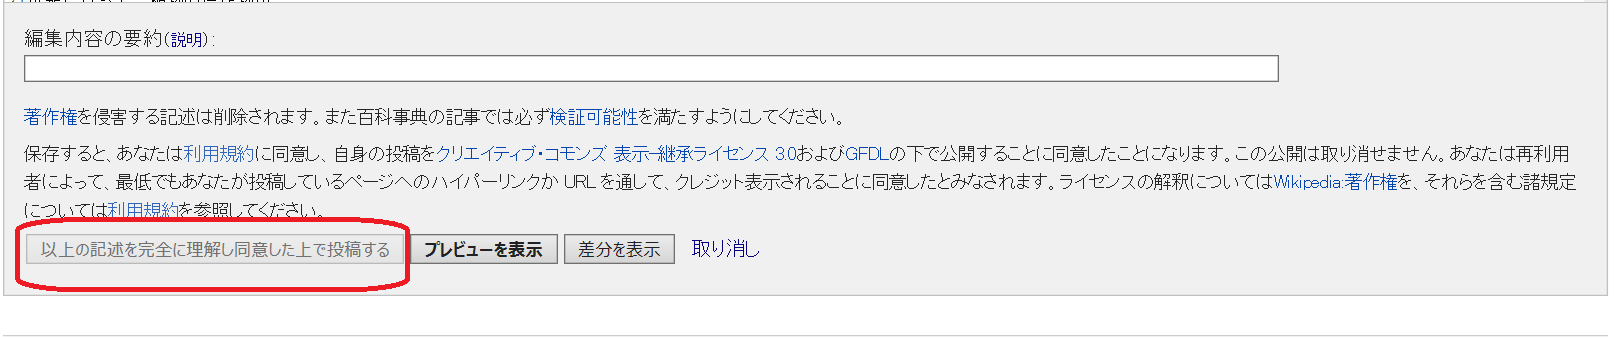
\includegraphics[width=15cm]{3.png}
\caption{編集画面3}\label{図}
\end{figure}

以上が編集の方法である.\cite{rensyuu}

\chapter{Mediawikiについて}
\section{本章の構成}
本章では,本研究で使用するMediawikiの基礎知識と使用方法について記述する.
\section{Mediawikiとは}
Mediawikiとは,GNU General Public Licenseで配布されるウィキソフトウェアである.PHPで書かれており,データベースとしてMySQLまたはPostgreSQLを使用する.MediaWikiはWikipediaのために作られたシステムで,Wikipediaを運営している.
ウィキメディア財団によって開発されているウィキペディアの為にMagnus Manskeらによって作成された.最初はUseModWikiを使用していたが,2002年1月25日に新しいバージョンに切替えられた. \cite{media}

wikiは,ネットワーク上で文書の書き換えがどこでもできるようになっているため,共同作業で文書を作成するのに向いている.この特徴から,wikiはコラボレーションツールやグループウェアであるとも評される.\cite{media}

%図の挿入
\begin{figure}[htb]
\centering
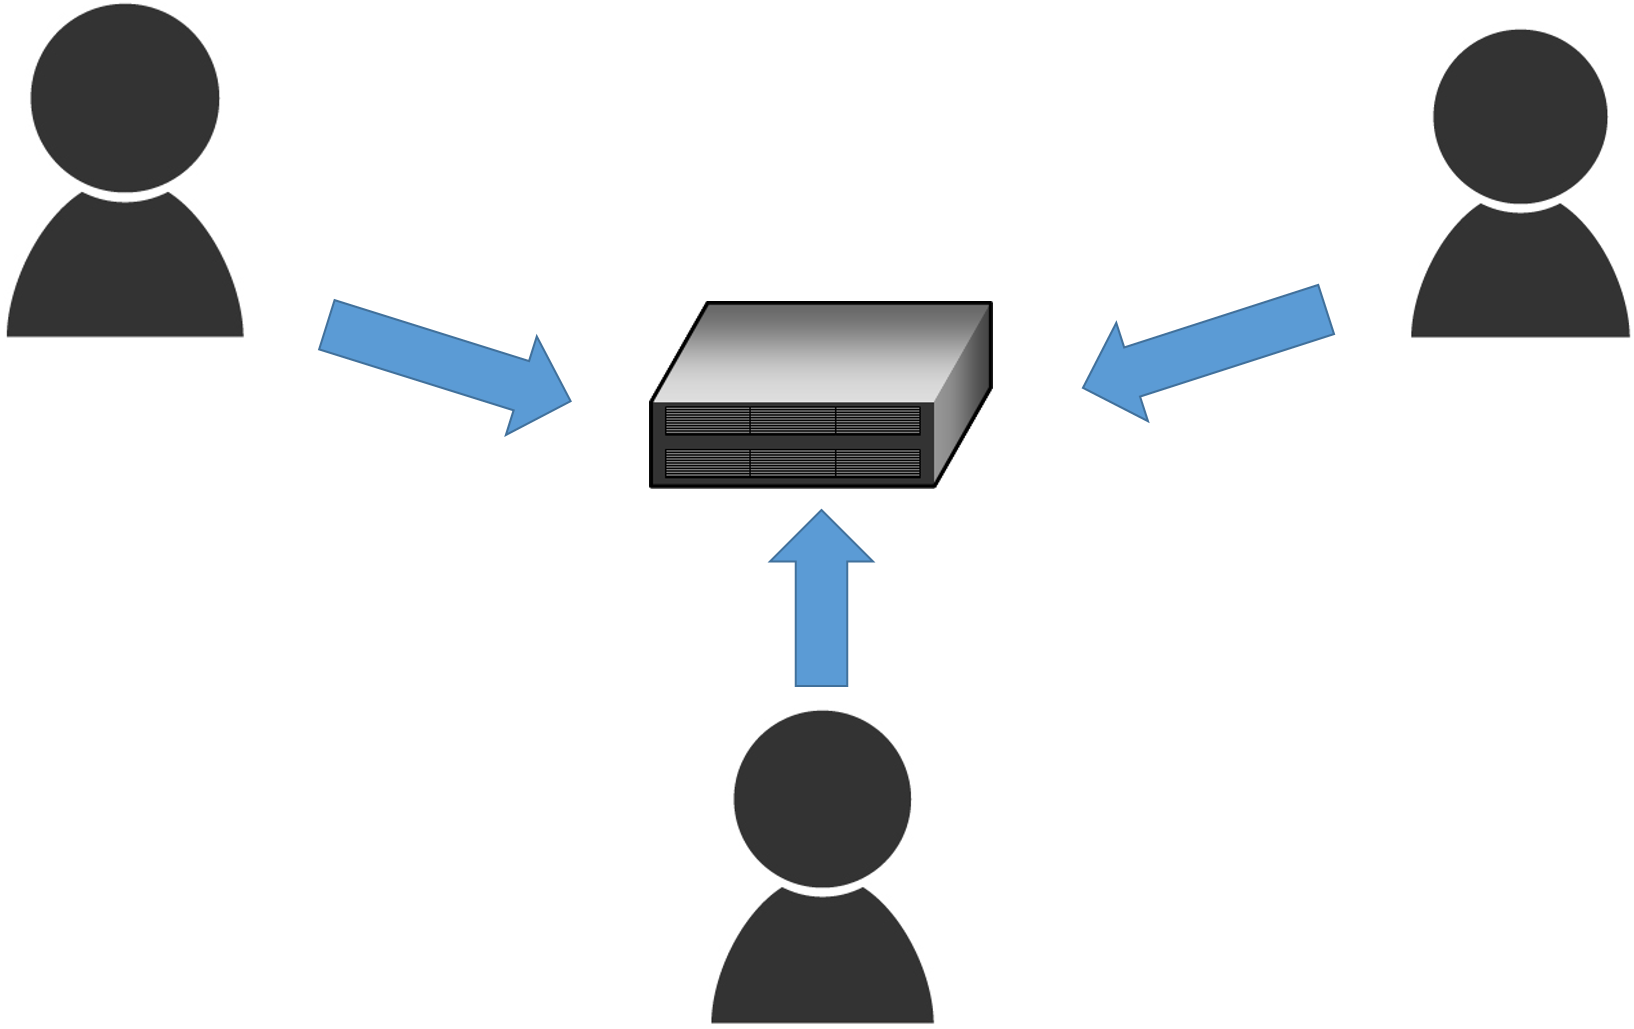
\includegraphics[width=15cm]{mediawiki}
\caption{Mediawakiイメージ図}\label{図}
\end{figure}

\section{特徴}
主なMediawikiの特徴は,6つ上げられる.
\begin{enumerate}
\item ネットワークがつながればどこからでも文章を書き換えることができる.
\item 登録が不必要で.誰でも書き換えることができいる.
\item HTMLなどの言語よりも簡潔なwiki特有の言語があるため覚えやすい.
\item 文書の書き換えは,ウェブプラウザでできるためツールなど揃える必要がない.
\item 同じwiki内にリンクが張りやすく連携がとりやすい.
\item 記事の編集のログを残すことができる.
\end{enumerate}
以上が主な特徴である.

\section{記事の作成方法}
Mediawikiの新規記事作成方法を説明する.

\subsection{新規作成}
記事のの新規作成方法は,さまざまにあるが,本稿では検索ページからの作成方法を説明する.

\begin{enumerate}
\item 作成したい記事の名前を入力して検索する.
\item 赤く表示されている単語をクリックする.
\item 記事を入力する.
\end{enumerate}
以上が作成方法である.
%図の挿入
\begin{figure}[htb]
\centering
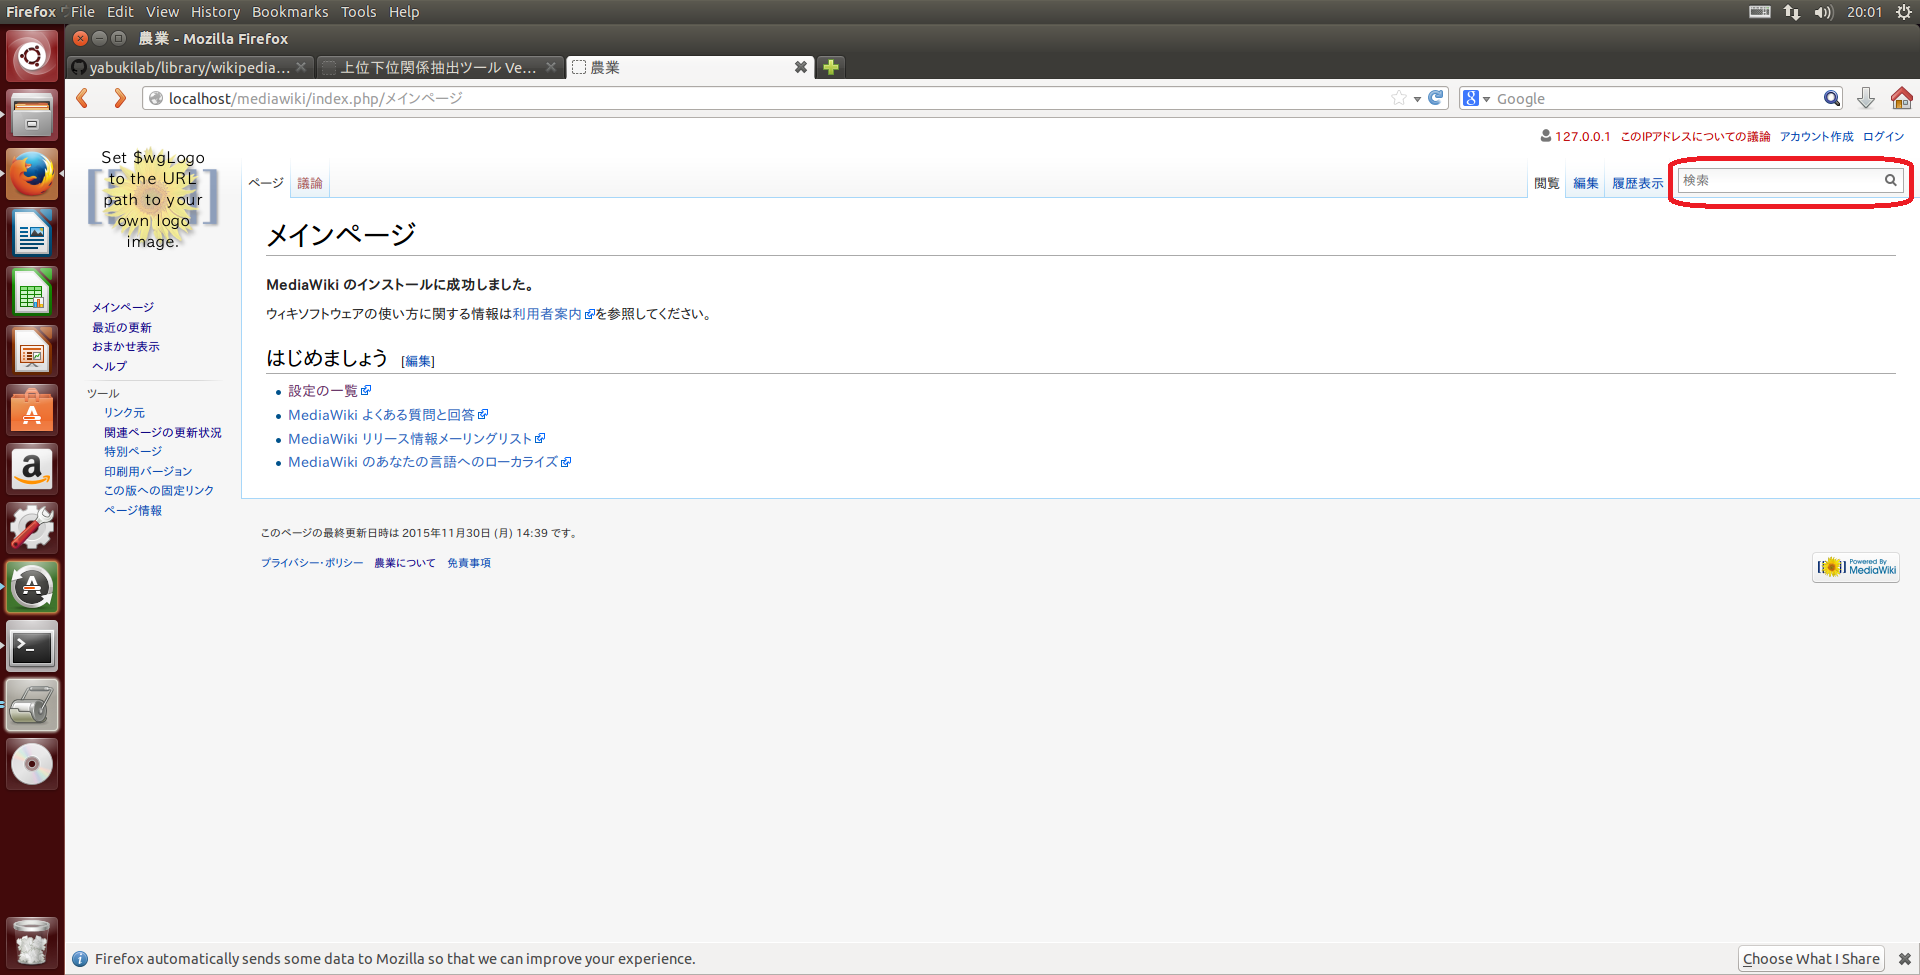
\includegraphics[width=15cm]{kensaku}
\caption{Mediawakiイメージ図2}\label{図}
\end{figure}


%図の挿入
\begin{figure}[htb]
\centering
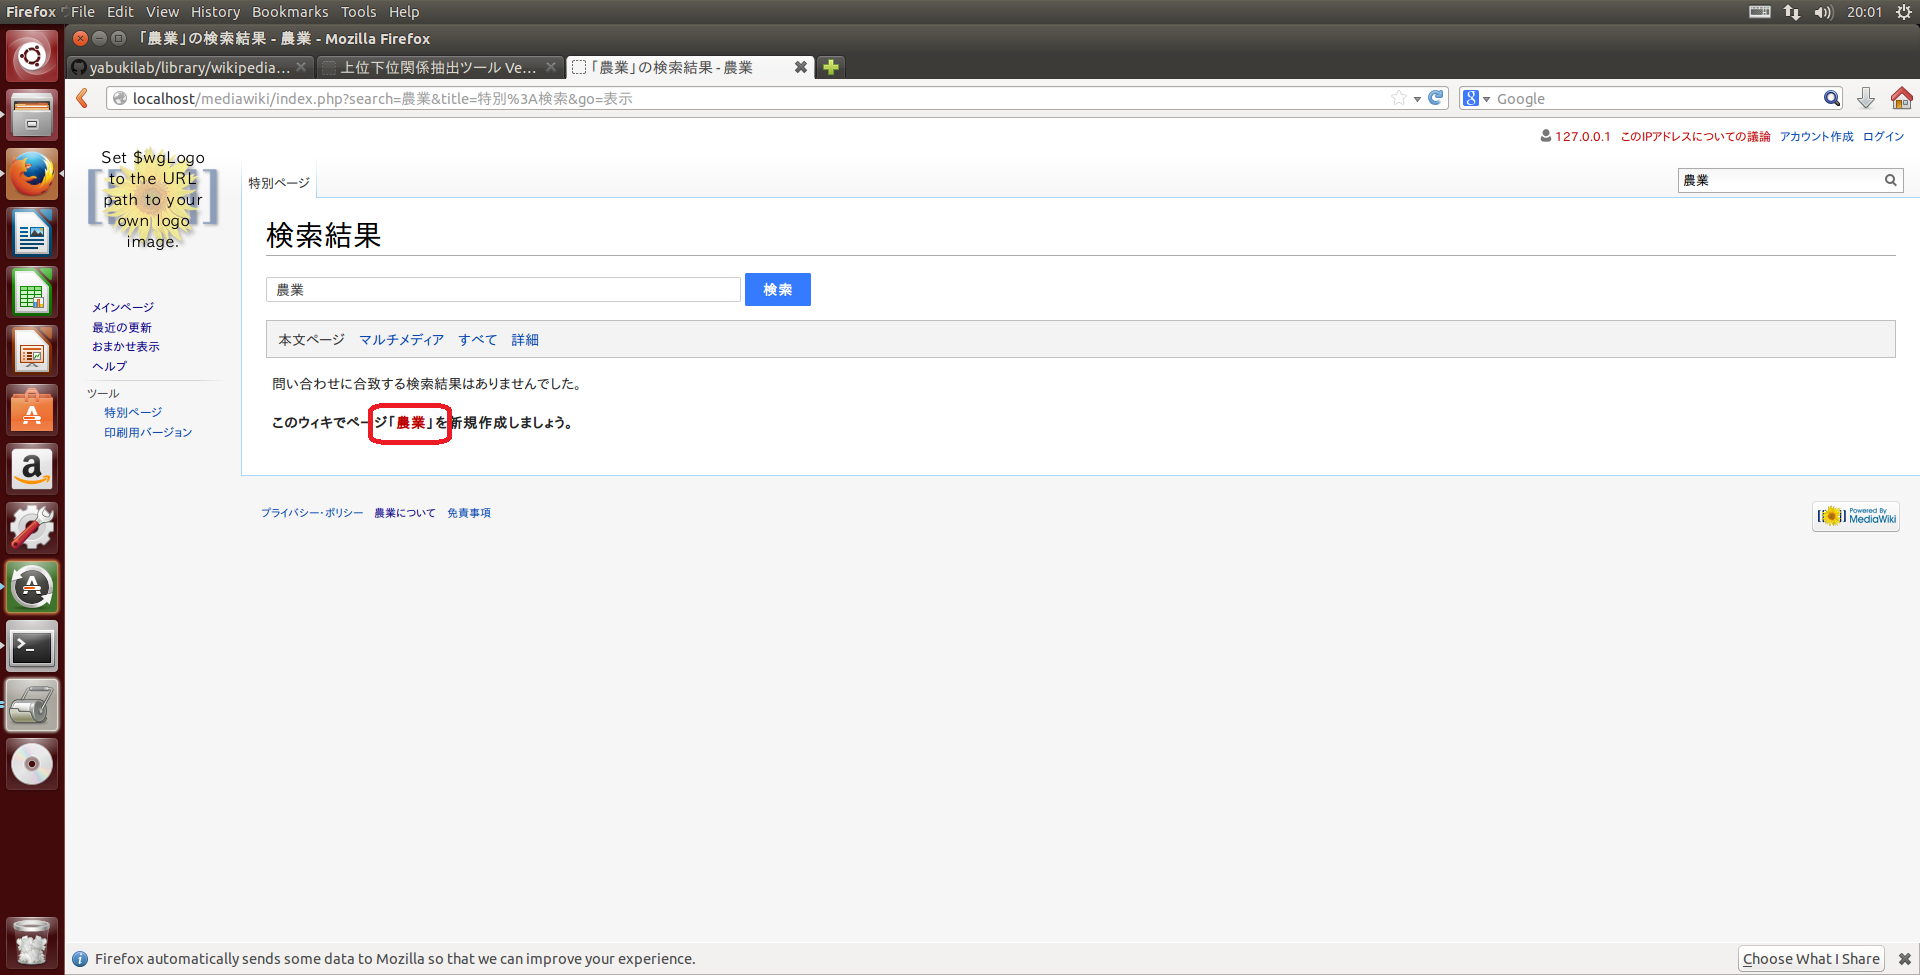
\includegraphics[width=15cm]{sakusei}
\caption{Mediawakiイメージ図3}\label{図}
\end{figure}



\section{編集方法}
Mediawikiの編集に必要な方法を説明する.

Mediawikiを編集するためには,ページの右上にある編集のタブを押す.次に記事を変更する.そして,最後にページを変更を押す.

以上が編集方法である.

%図の挿入
\begin{figure}[htb]
\centering
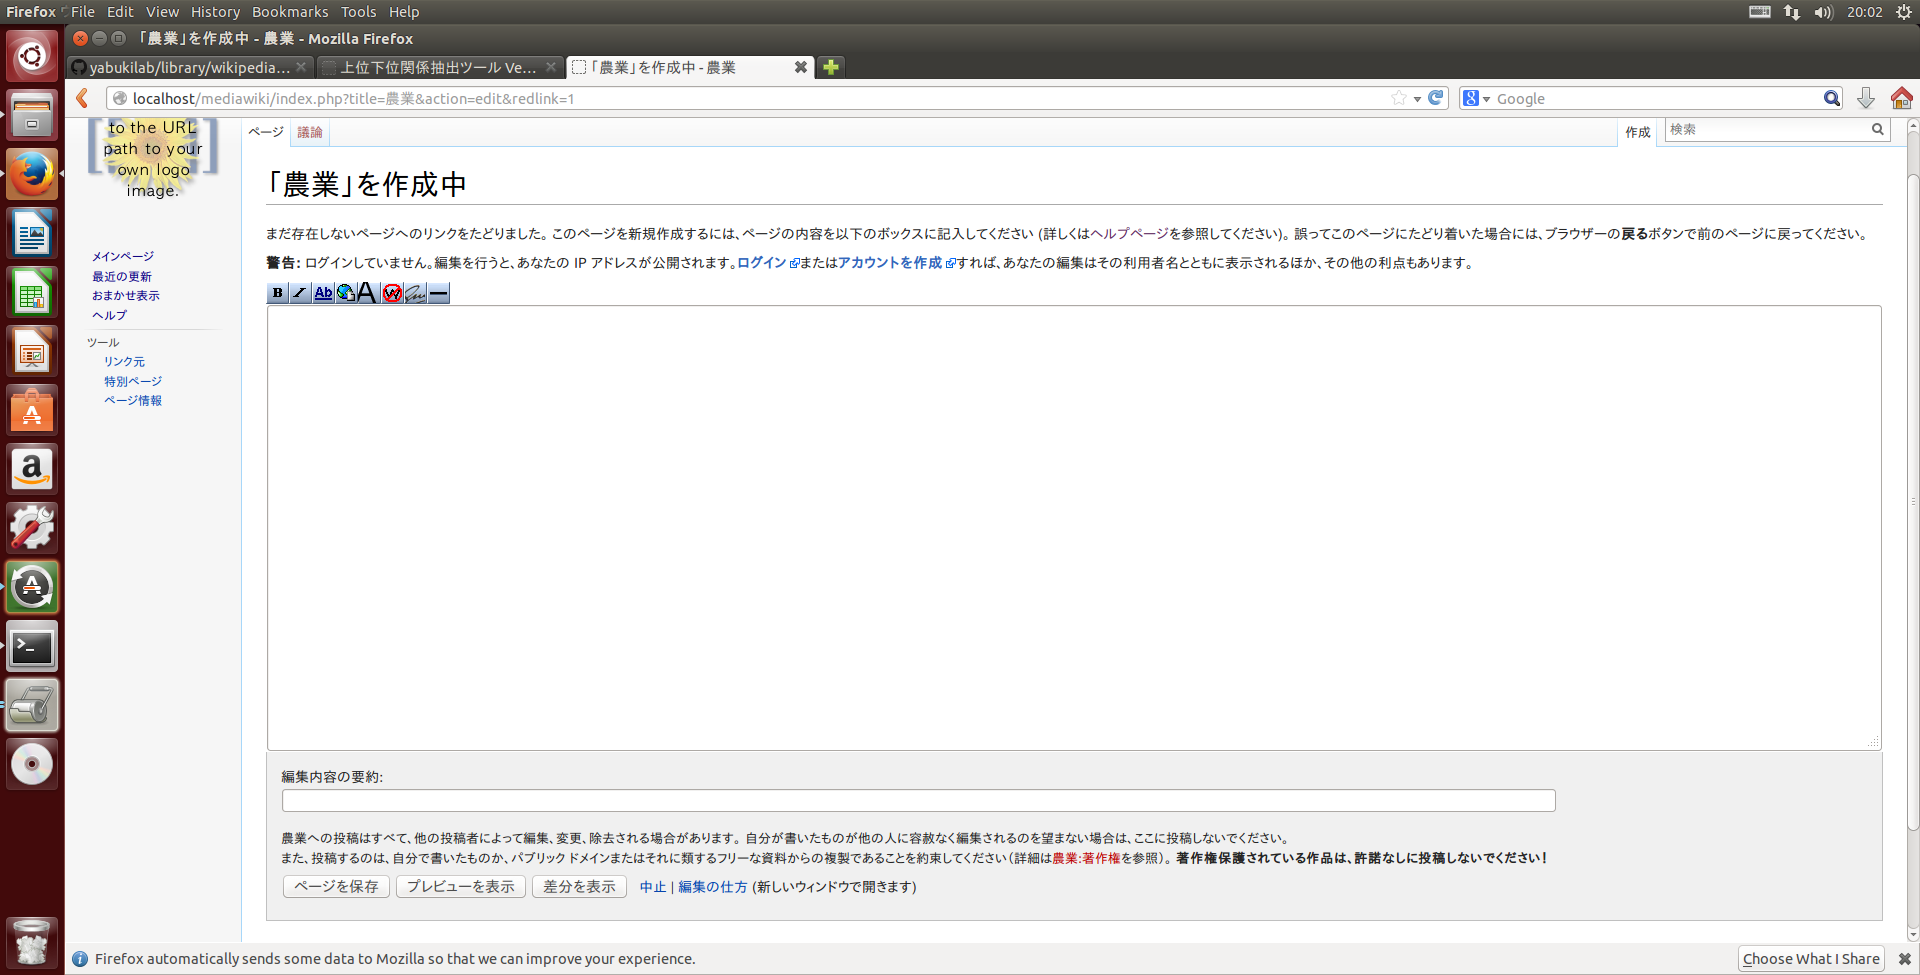
\includegraphics[width=15cm]{ubuntu}
\caption{Mediawaki編集画面}\label{図}
\end{figure}


\clearpage

\section{書式整形}
ウィキマークアップを使用することによりテキストの整形ができる.テキスト整形マークアップには,アスタリスク・シングルクォート・等号などごく一般的な記号を使用する\cite{help}.

Wikiを編集するために必要な書式整形とその意味と効果について説明を行う.

\subsection{太字}

太字は,語句を強調するために使う.太字のテキストは,「'''太字'''」と表示する.


%図の挿入
\begin{figure}[htb]
\centering
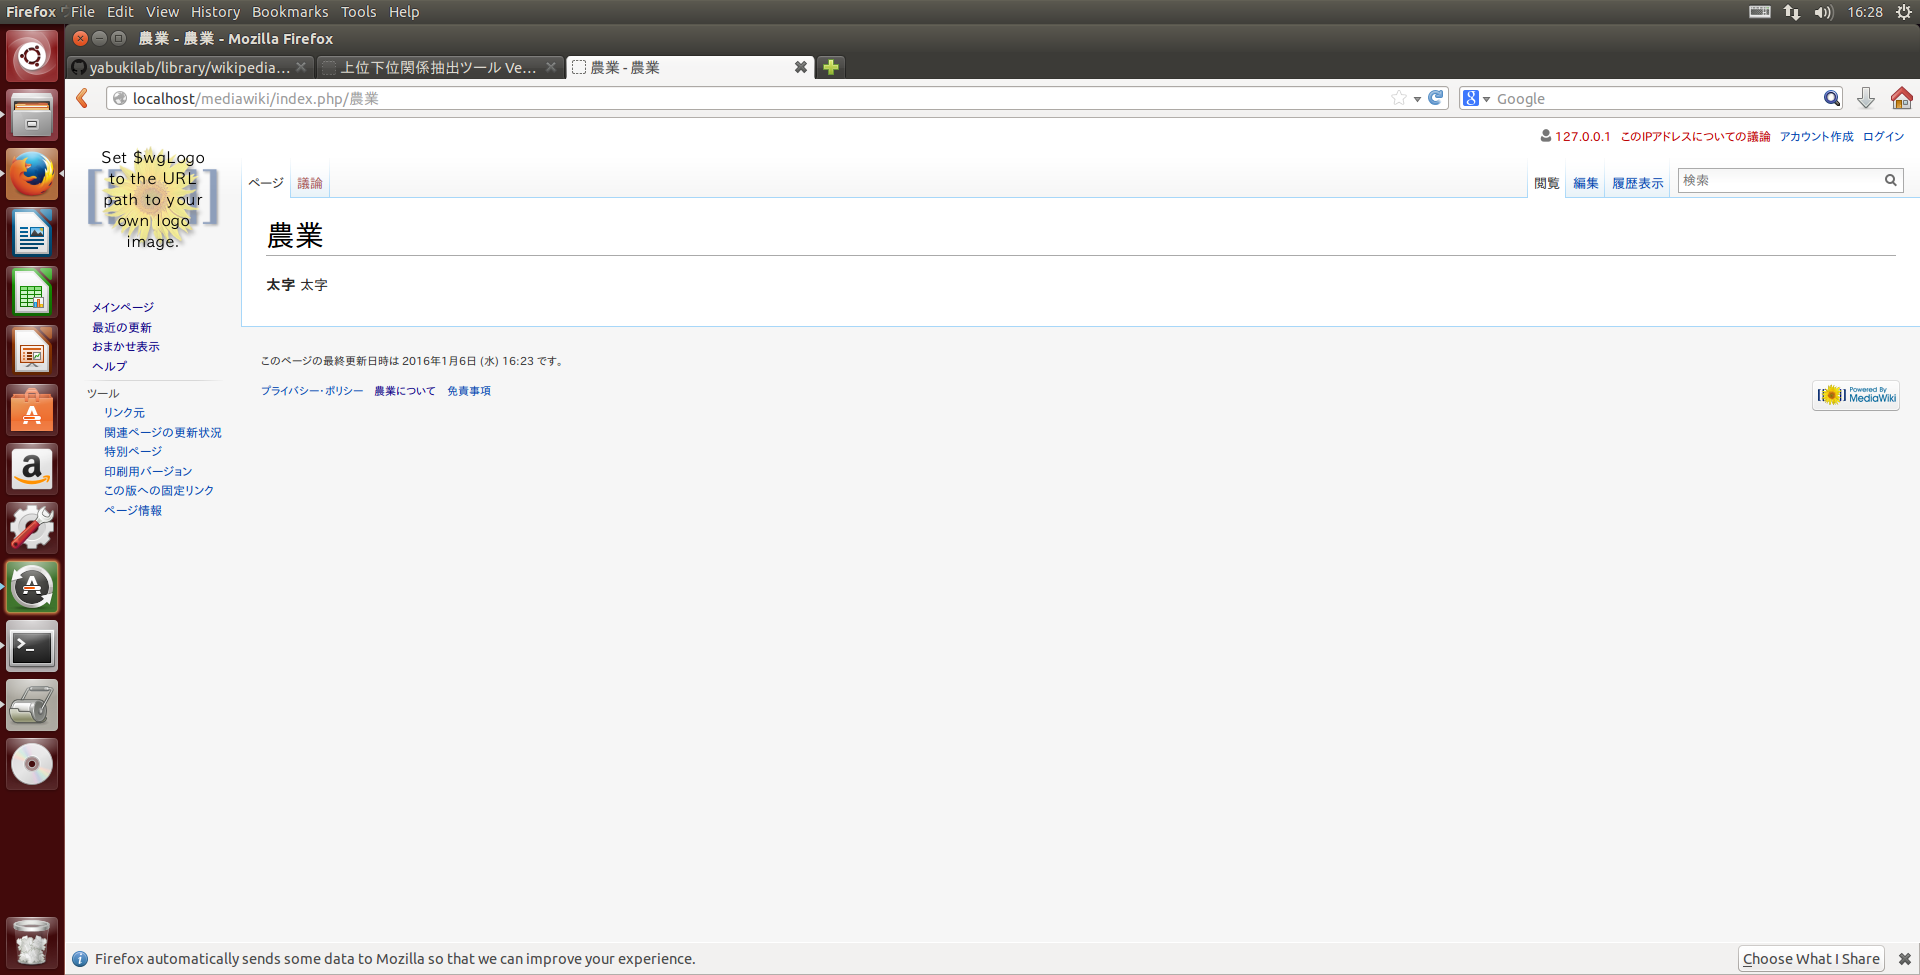
\includegraphics[width=15cm]{hutomozi}
\caption{太字}\label{図}
\end{figure}

\subsection{斜体}
斜体は,傾いた書体のことである.語句や文字を強調するために使う.斜体のテキストは,「''斜体''」と表示する.

%図の挿入
\begin{figure}[htb]
\centering
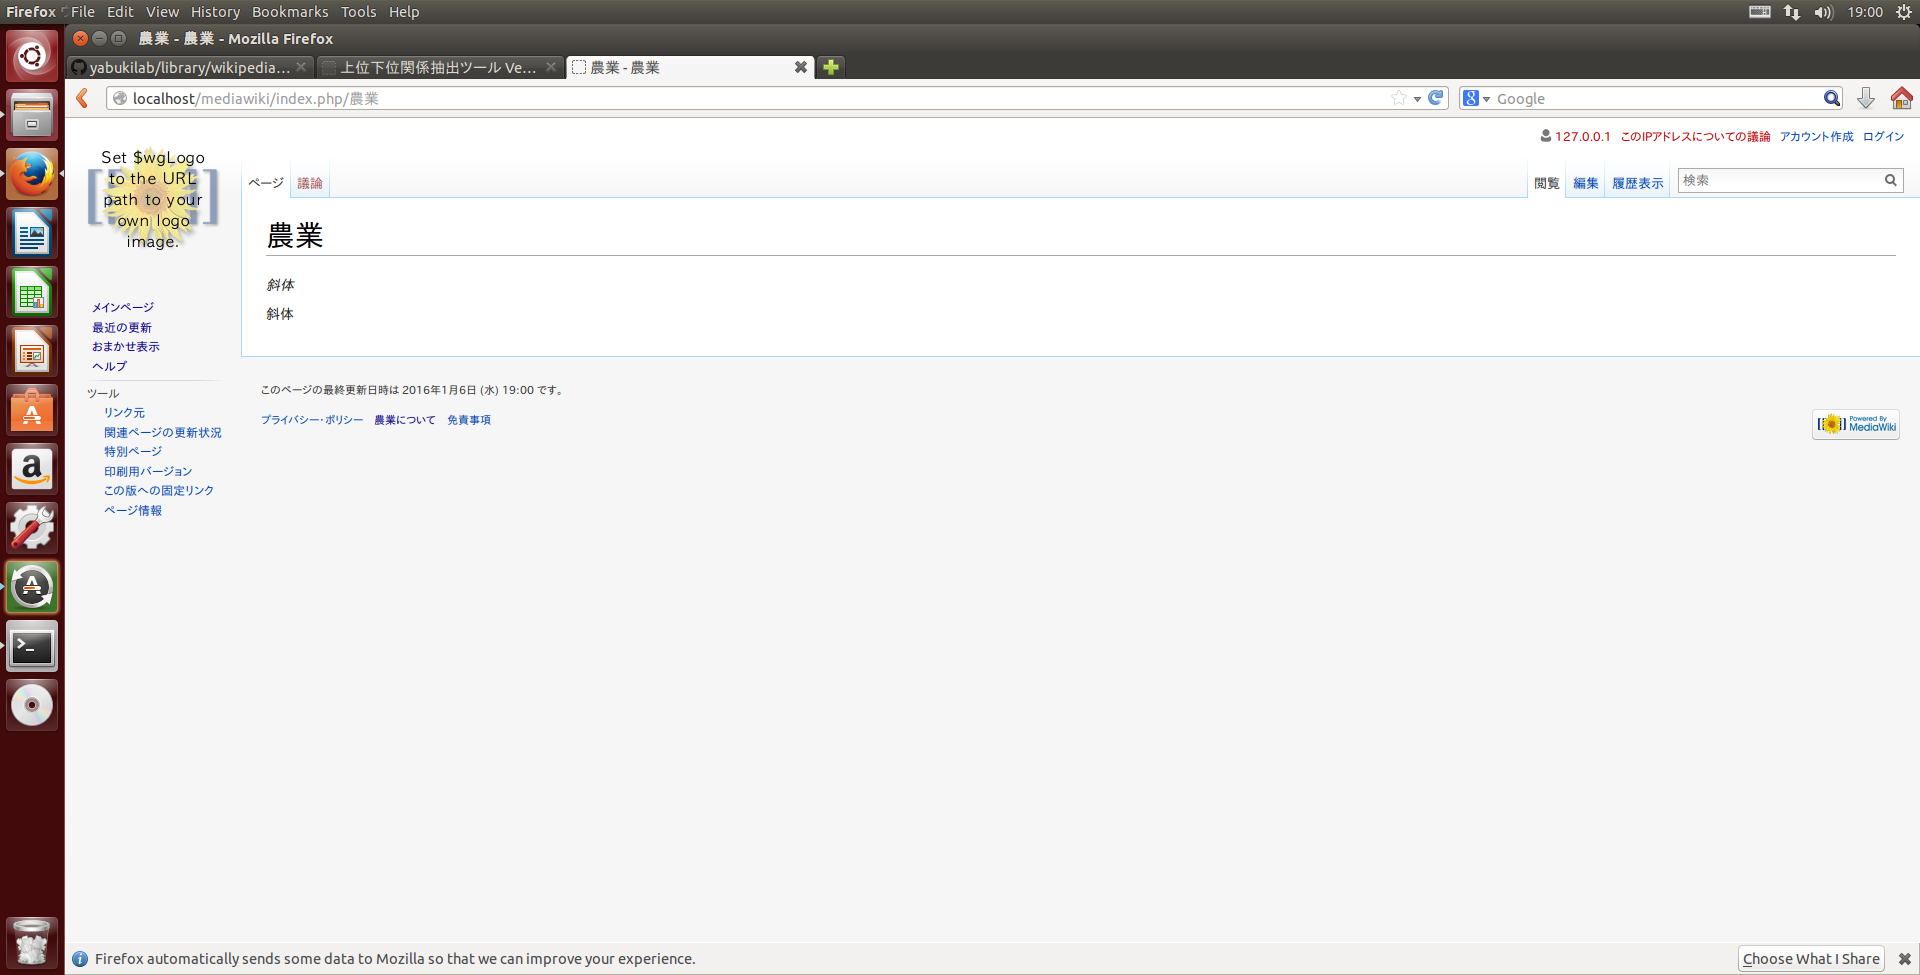
\includegraphics[width=14cm]{syatai}
\caption{斜体}\label{図}
\end{figure}


\subsection{太字と斜体}

太字と斜体のどちらも表示させる場合は,「'''''太字'''''」と「'」を太字と斜体を合計した数を表示することで生成する.

%図の挿入
\begin{figure}[htb]
\centering
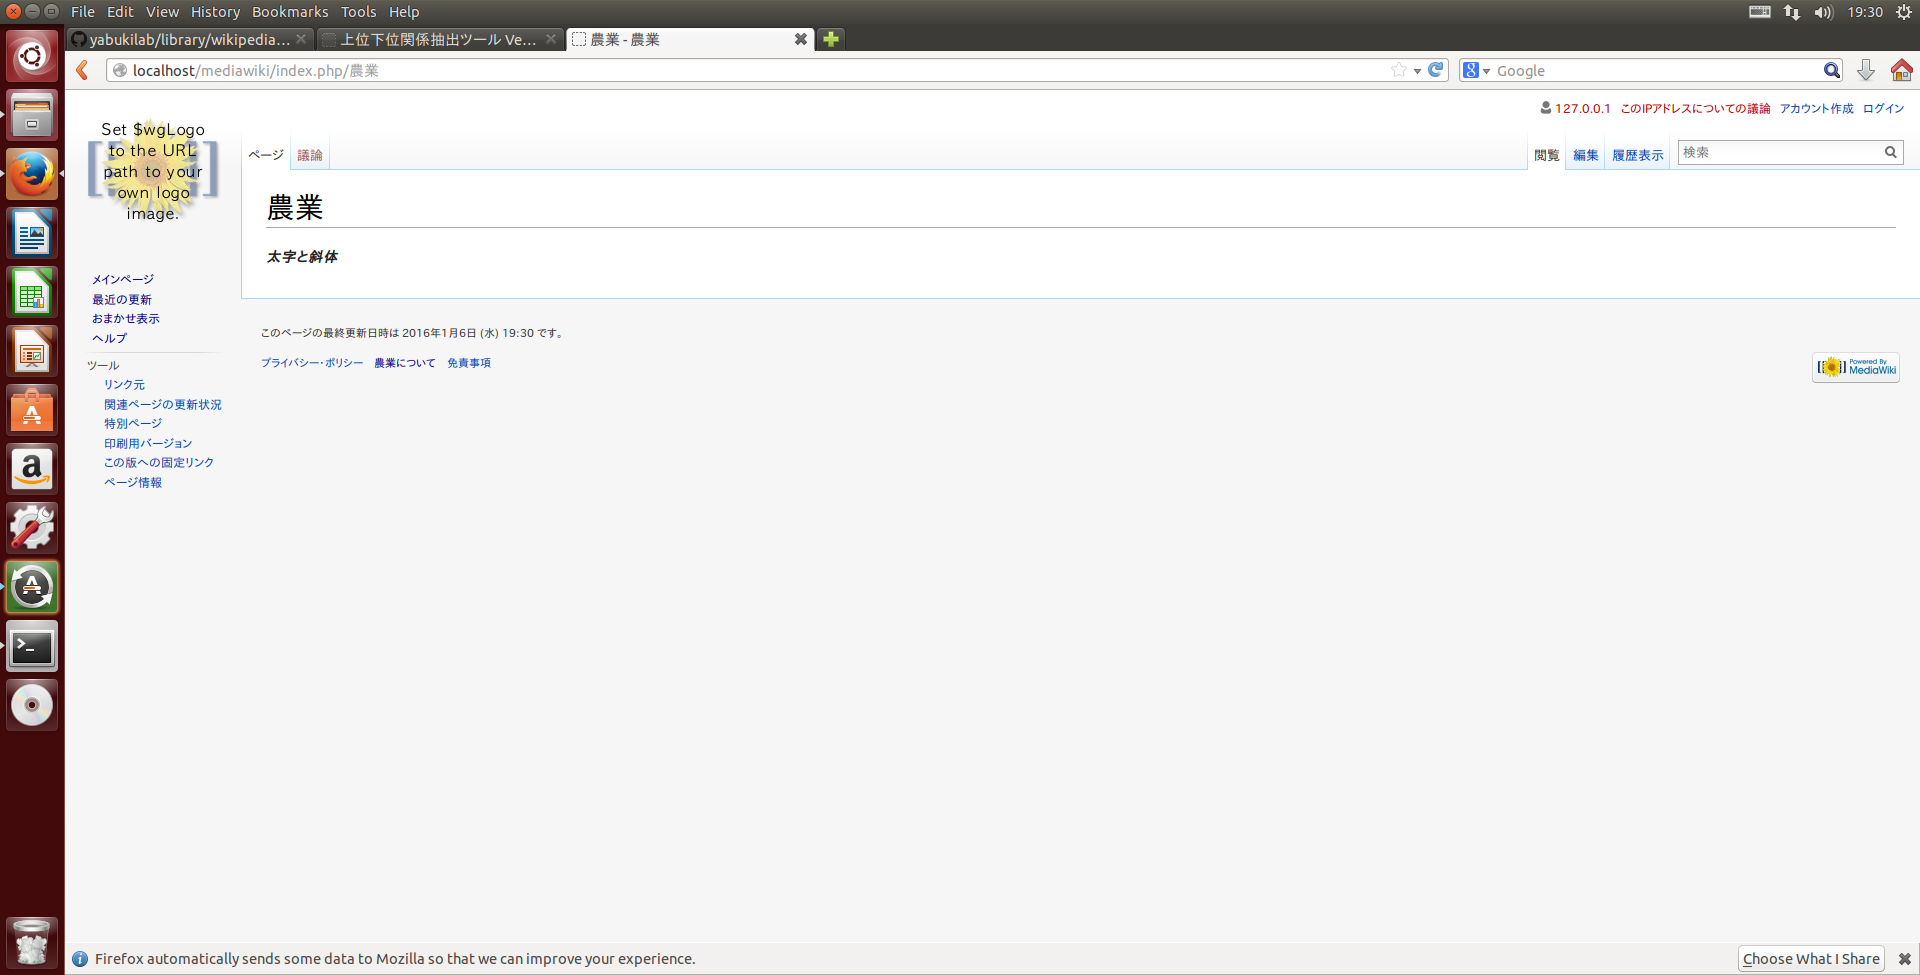
\includegraphics[width=14cm]{hutosya}
\caption{太字と斜体}\label{図}
\end{figure}


\subsection{取り消し線}
取り消し線は書いた内容を訂正や取り消す場合に使う.書いた内容をあえて訂正を残しておきたい場合に使用する.取り消し線を表示させるには,<strike> 取り消し線 </strike>と表示する.

%図の挿入
\begin{figure}[htb]
\centering
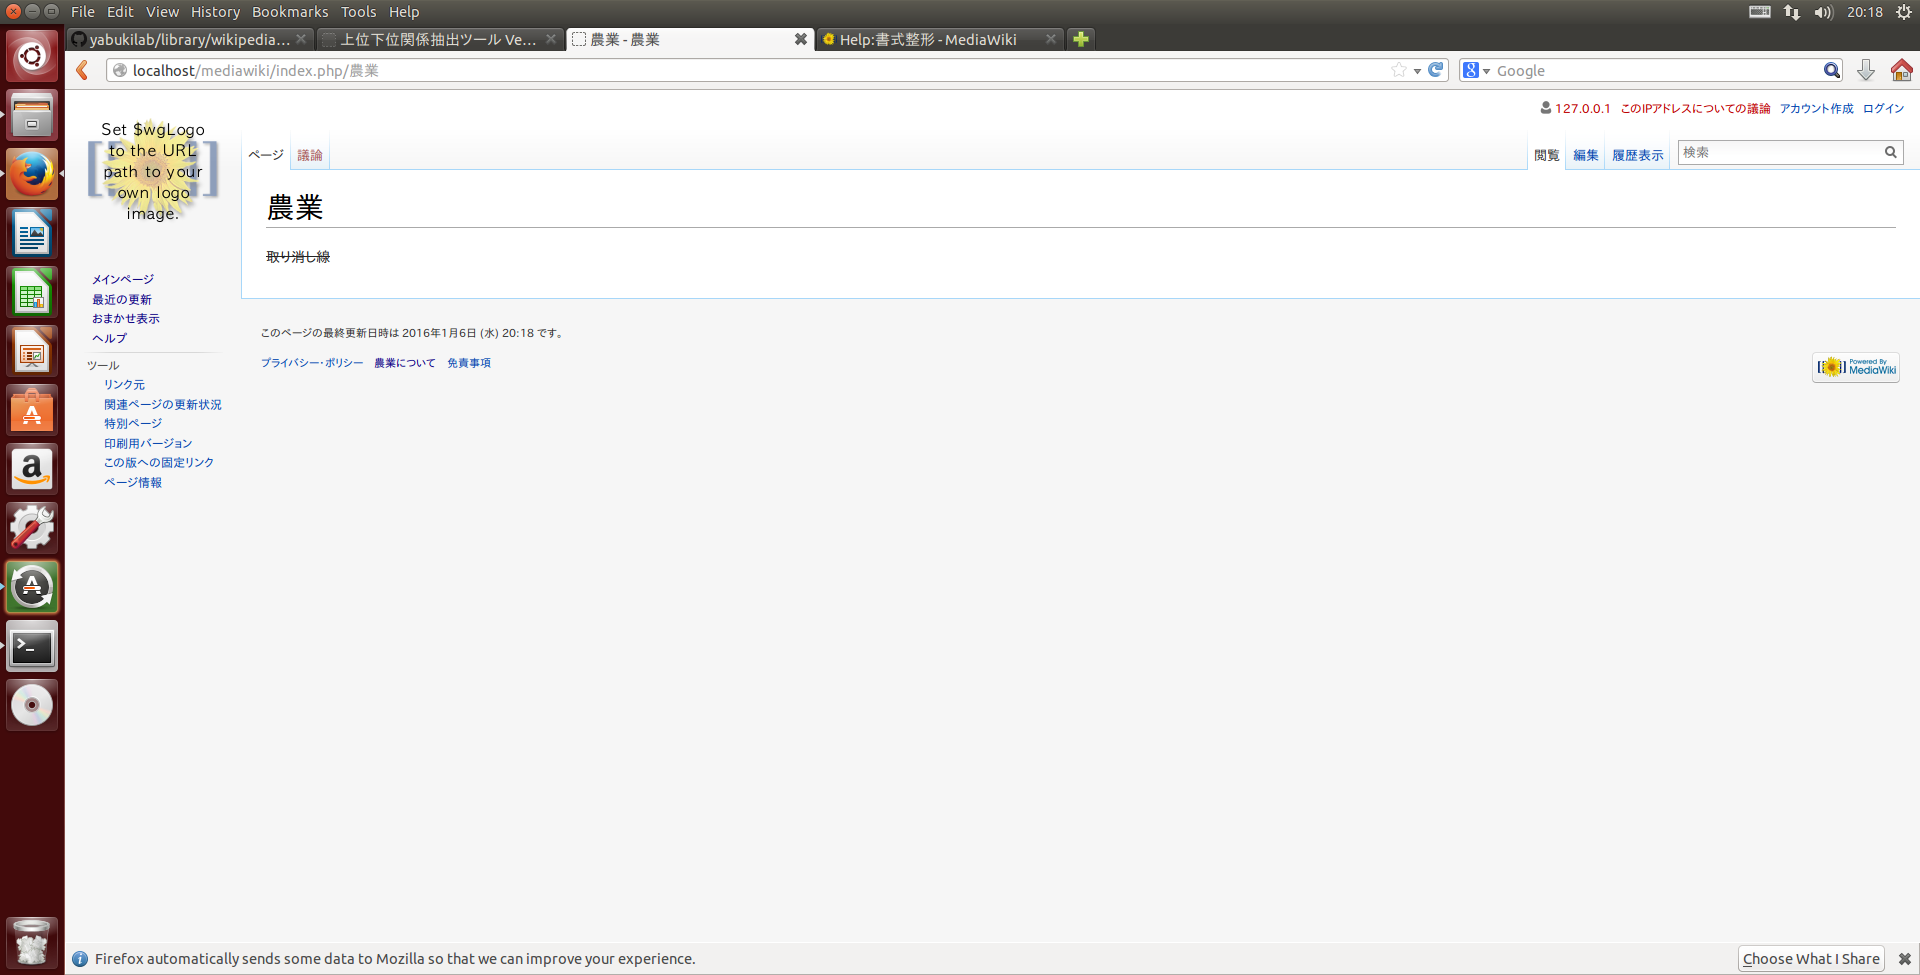
\includegraphics[width=14cm]{torikesi}
\caption{取り消し線}\label{図}
\end{figure}

\subsection{ウィキ マークアップの回避}
ウィキ内のマークアップを回避回避する場合に使う.ウィキ マークアップの回避をするには,<nowiki>''マークアップ''なし</nowiki>と表示する.

%図の挿入
\begin{figure}[htb]
\centering
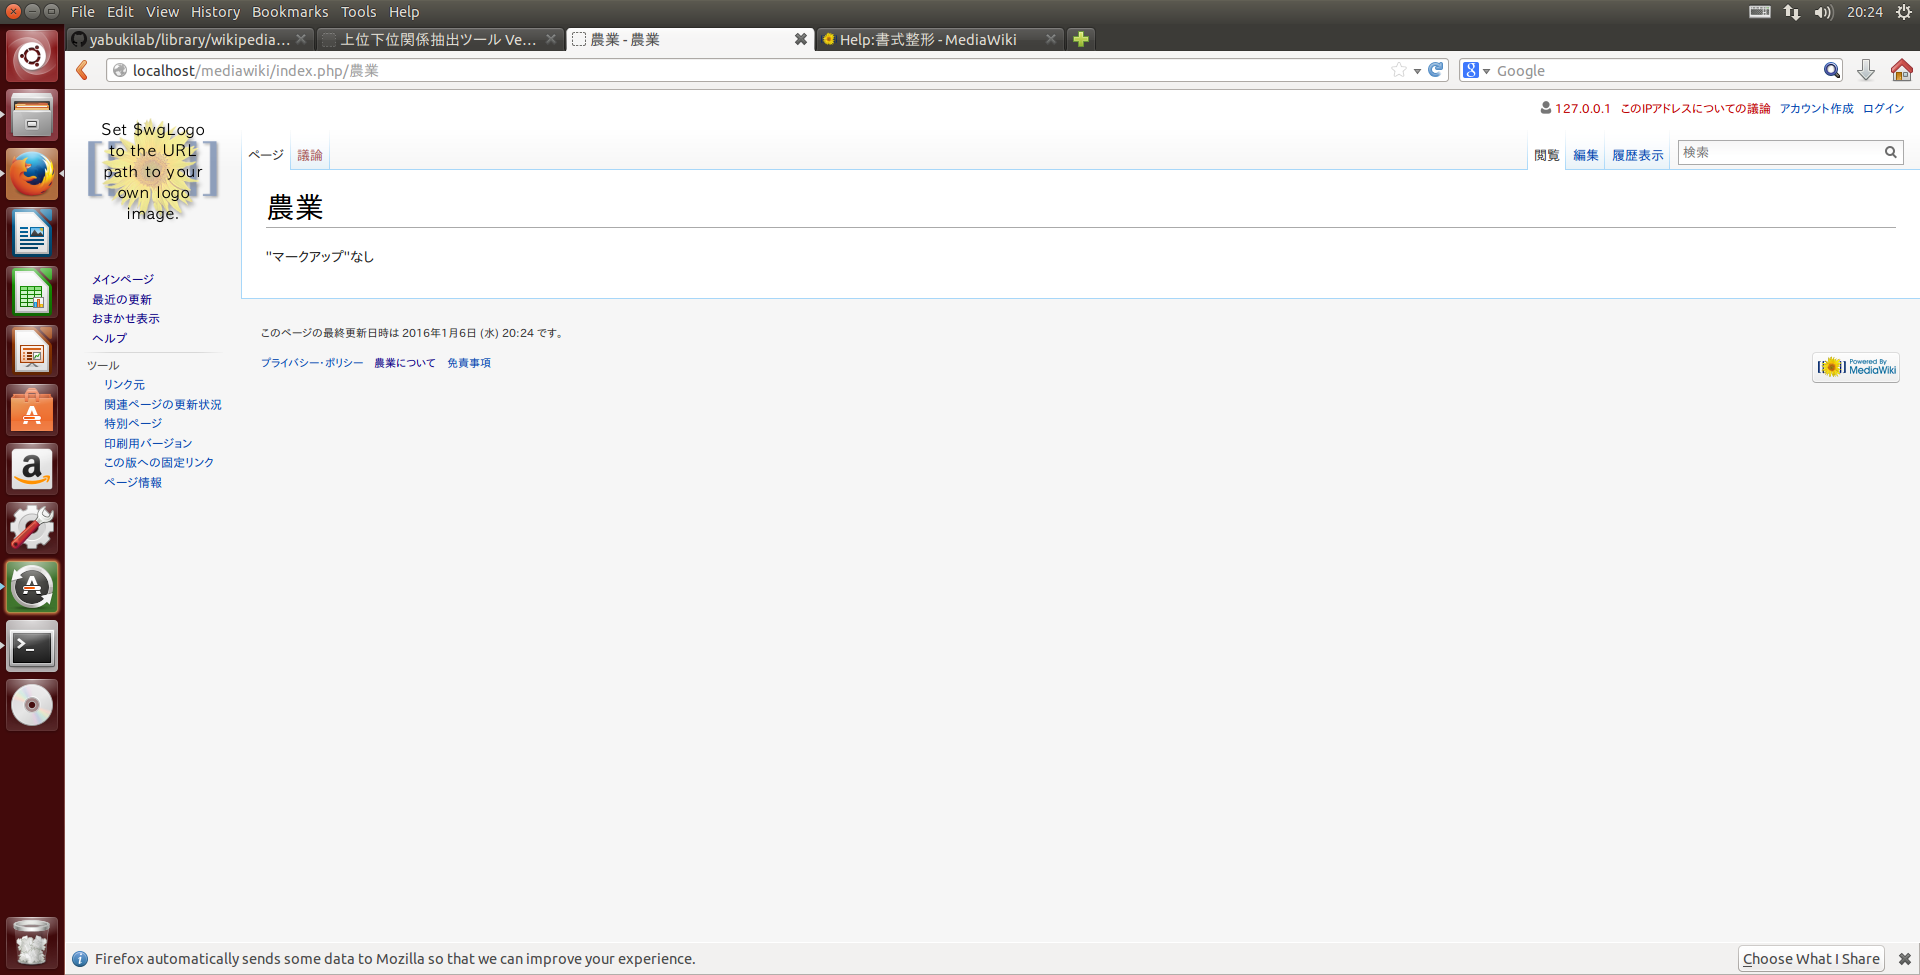
\includegraphics[width=14cm]{ma-ku}
\caption{ウィキ マークアップの回避}\label{図}
\end{figure}

\subsection{レベルの見出し}

レベルごとに見出しを分けていくには.「== レベル 2 ==」と「=== レベル 3 ===」というように「=」を左右に1つずつ増やしていく.これをレベル4まで続けると自動的に目次が生成される.


%図の挿入
\begin{figure}[htb]
\centering
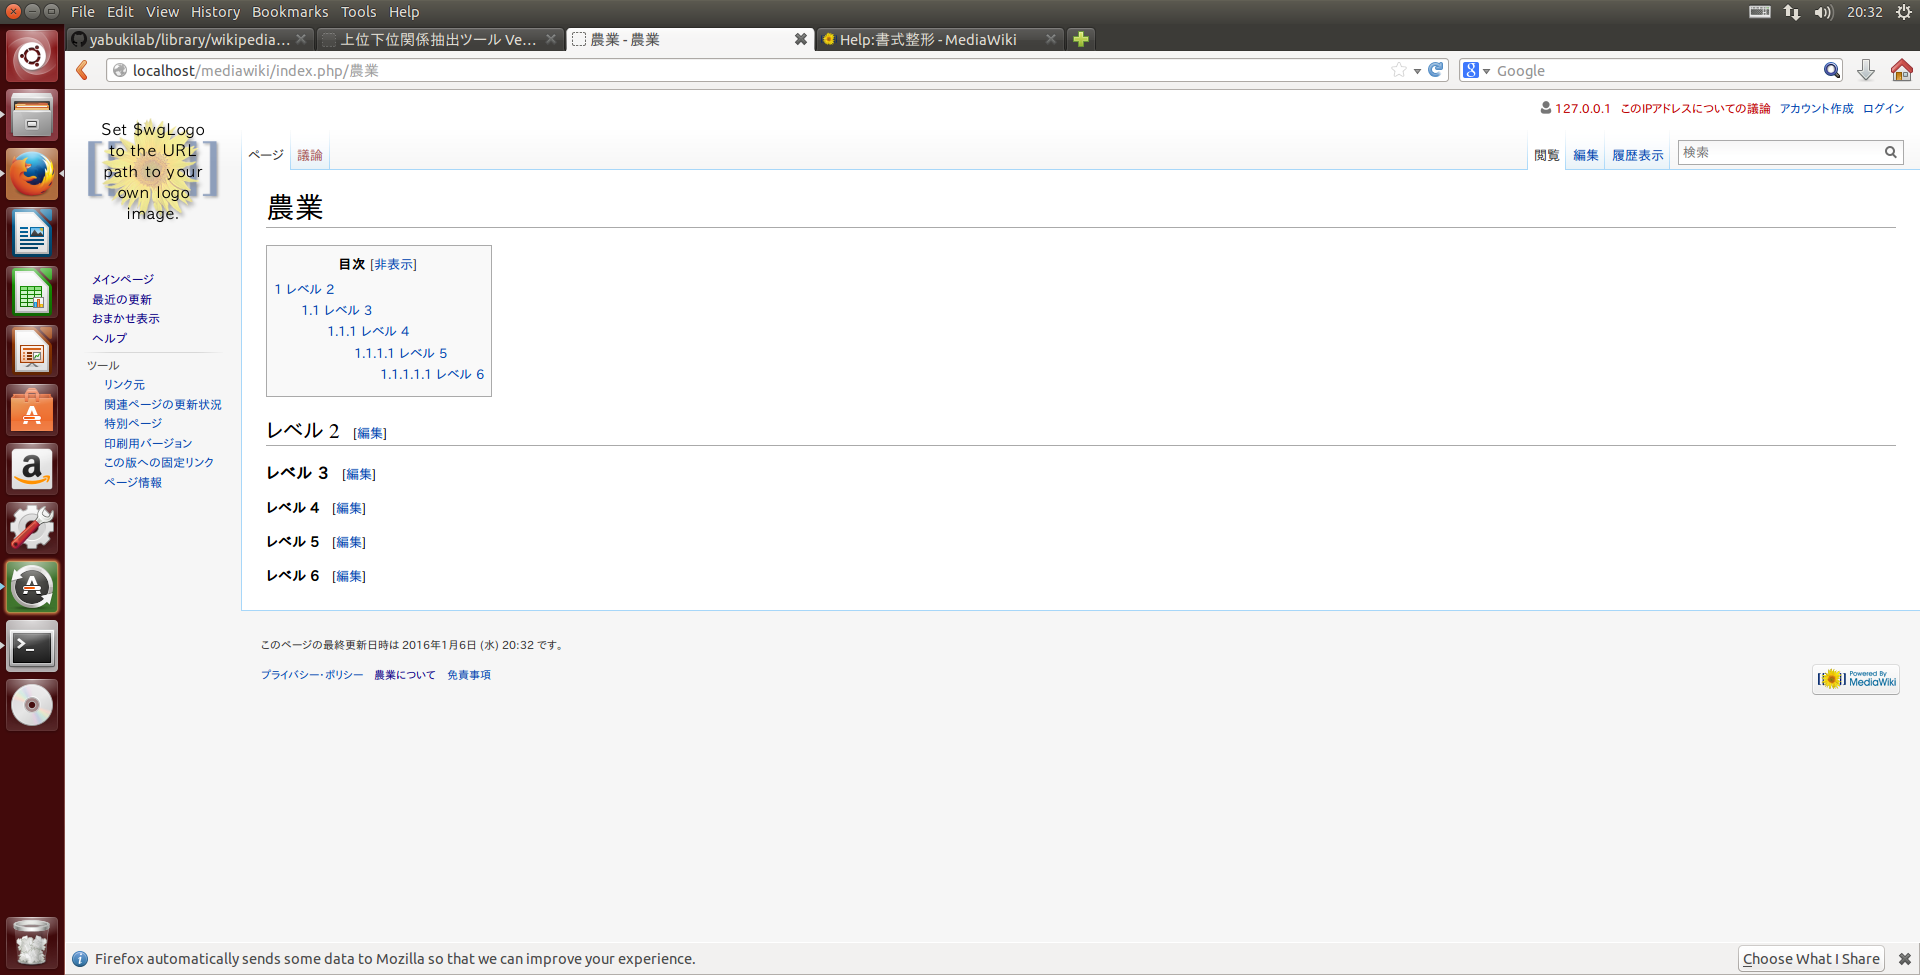
\includegraphics[width=14cm]{reberu}
\caption{レベルの見出し}\label{図}
\end{figure}

\subsection{水平線}
水平線は,文を区切り,次の文に進める場合に使用する.水平線を表示するには,「----」を文と文の間に表示する.


%図の挿入
\begin{figure}[htb]
\centering
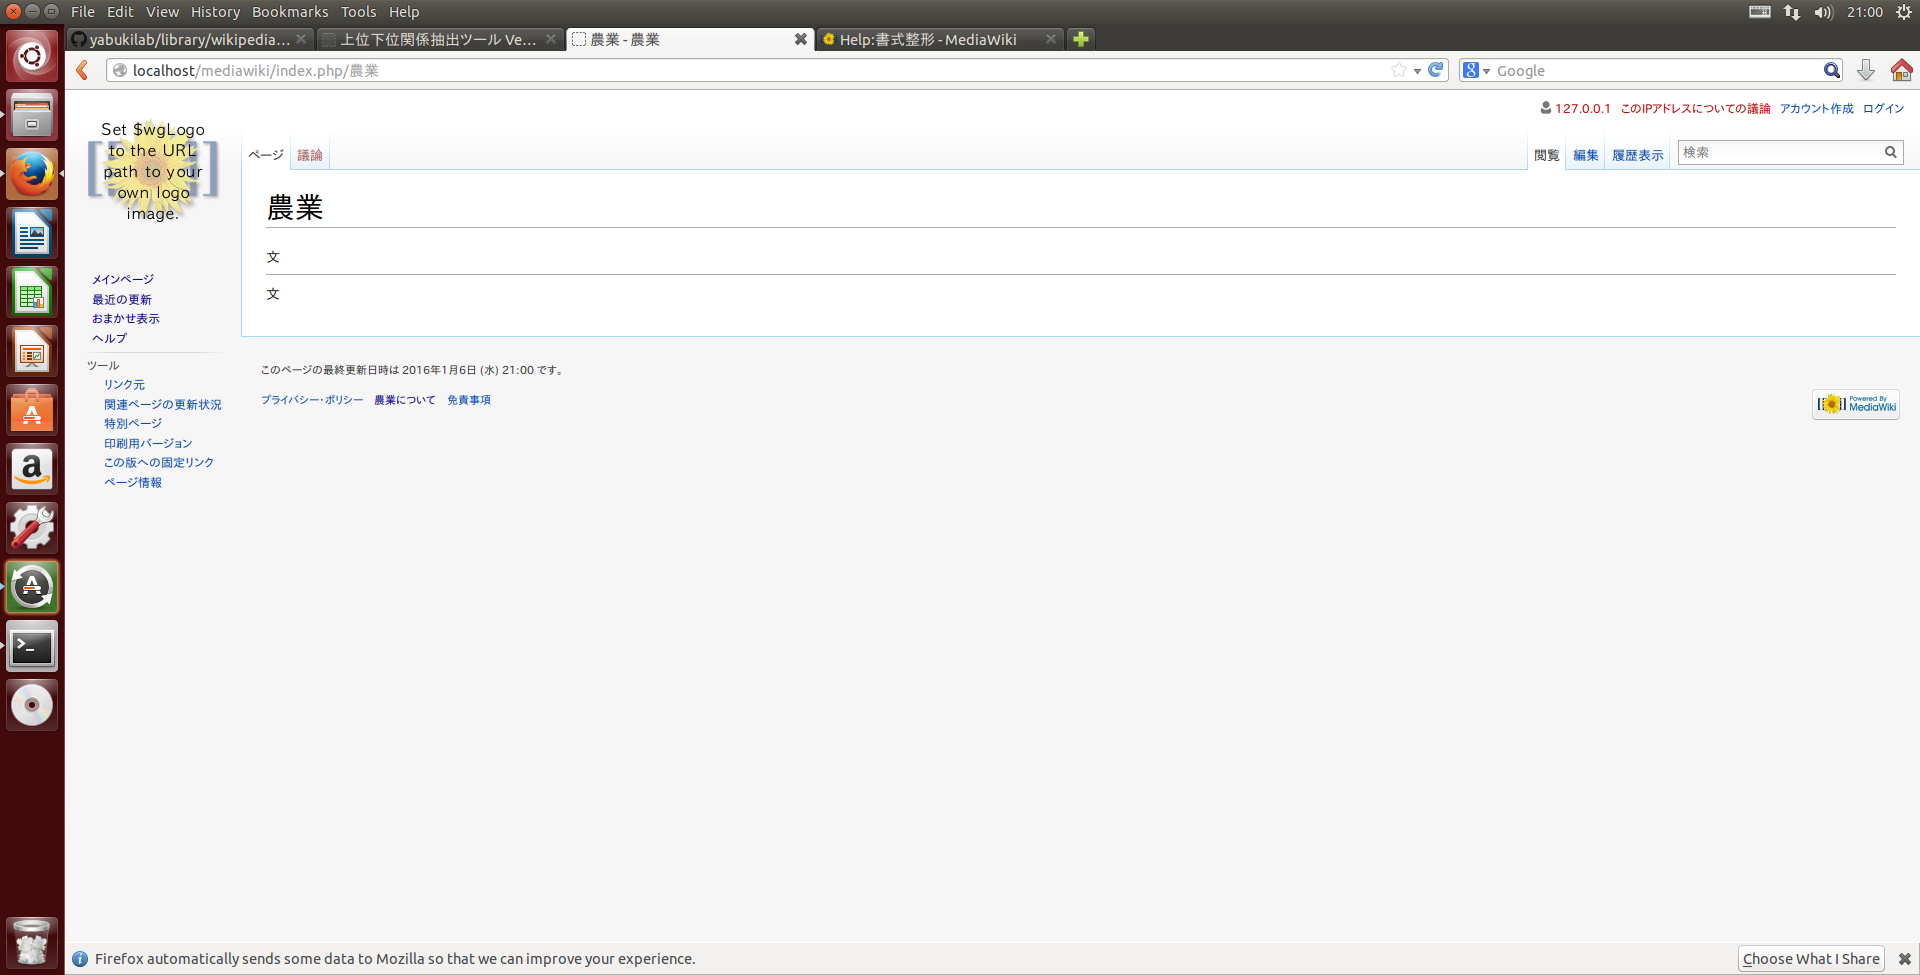
\includegraphics[width=14cm]{suihei}
\caption{水平線}\label{図}
\end{figure}

\subsection{箇条書き}
文を箇条書きする場合に使用する.箇条書きを表示するには,「*」で文を始める.「**」とアスタリスクが多いほどリストが深くなっていく.

%図の挿入
\begin{figure}[htb]
\centering
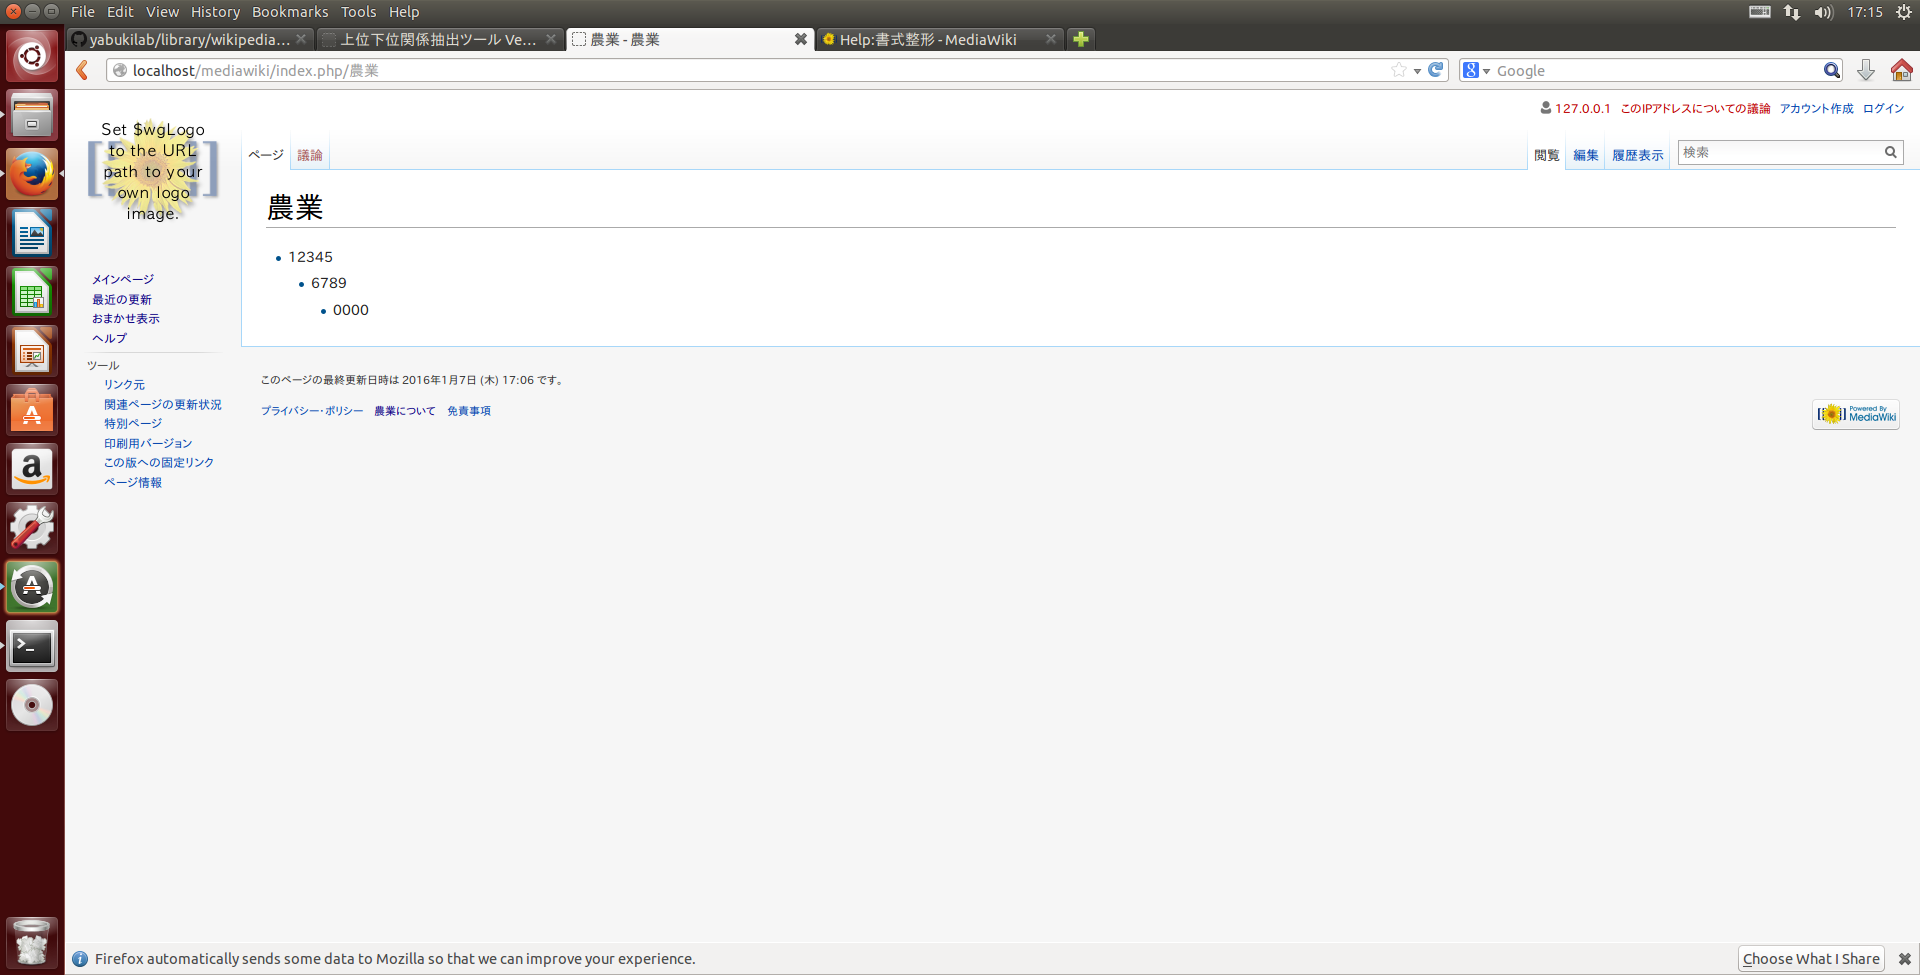
\includegraphics[width=14cm]{kazyou}
\caption{箇条書き}\label{図}
\end{figure}

\subsection{番号付きリスト}

番号付きリストは,番号をつけたいリストを作成する時に使用する.番号付きリストは,「ナンバーサイン」で文を始める.ナンバーサインを2つなど多いほどリストが深くなっていく.

%図の挿入
\begin{figure}[htb]
\centering
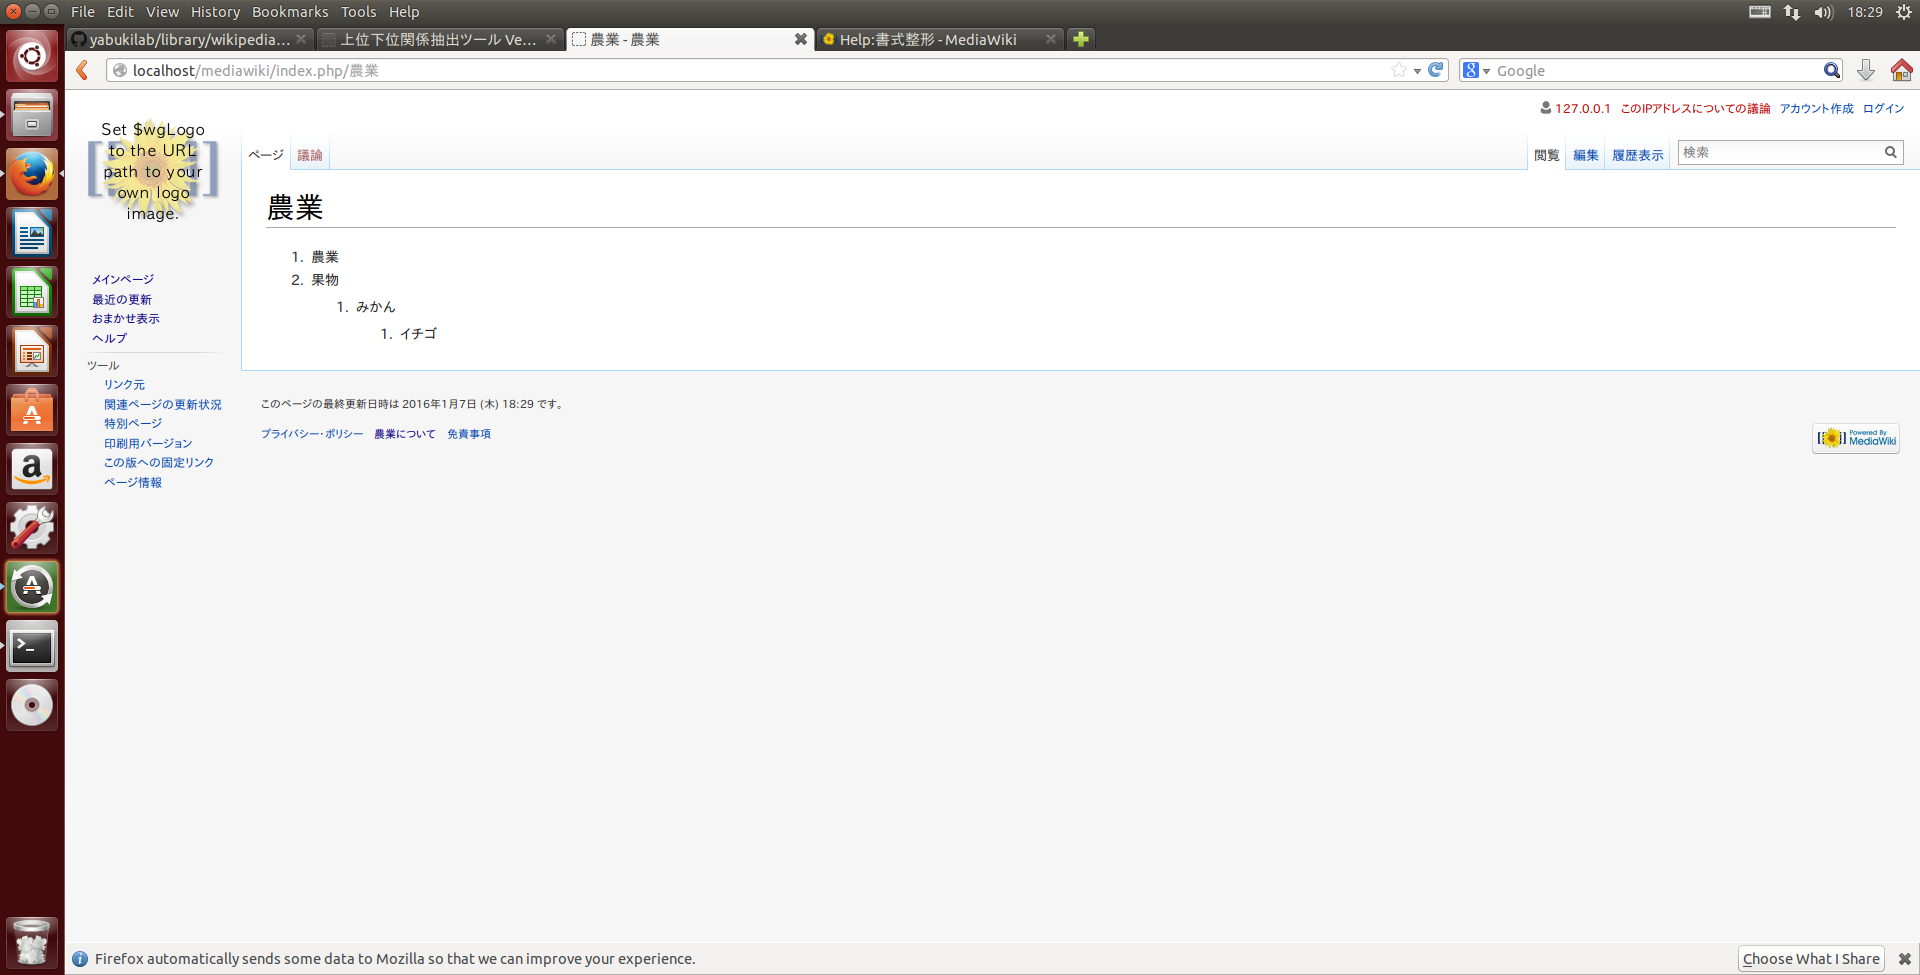
\includegraphics[width=14cm]{risuto}
\caption{番号付きリスト}\label{図}
\end{figure}

\subsection{定義リスト}
定義リストは,語句とその意味や説明を文にしてリスト化したものである.定義リストは,1行目の先頭に「;」を設置して,2行目の先頭に「:」に設置して表示する.

%図の挿入
\begin{figure}[htb]
\centering
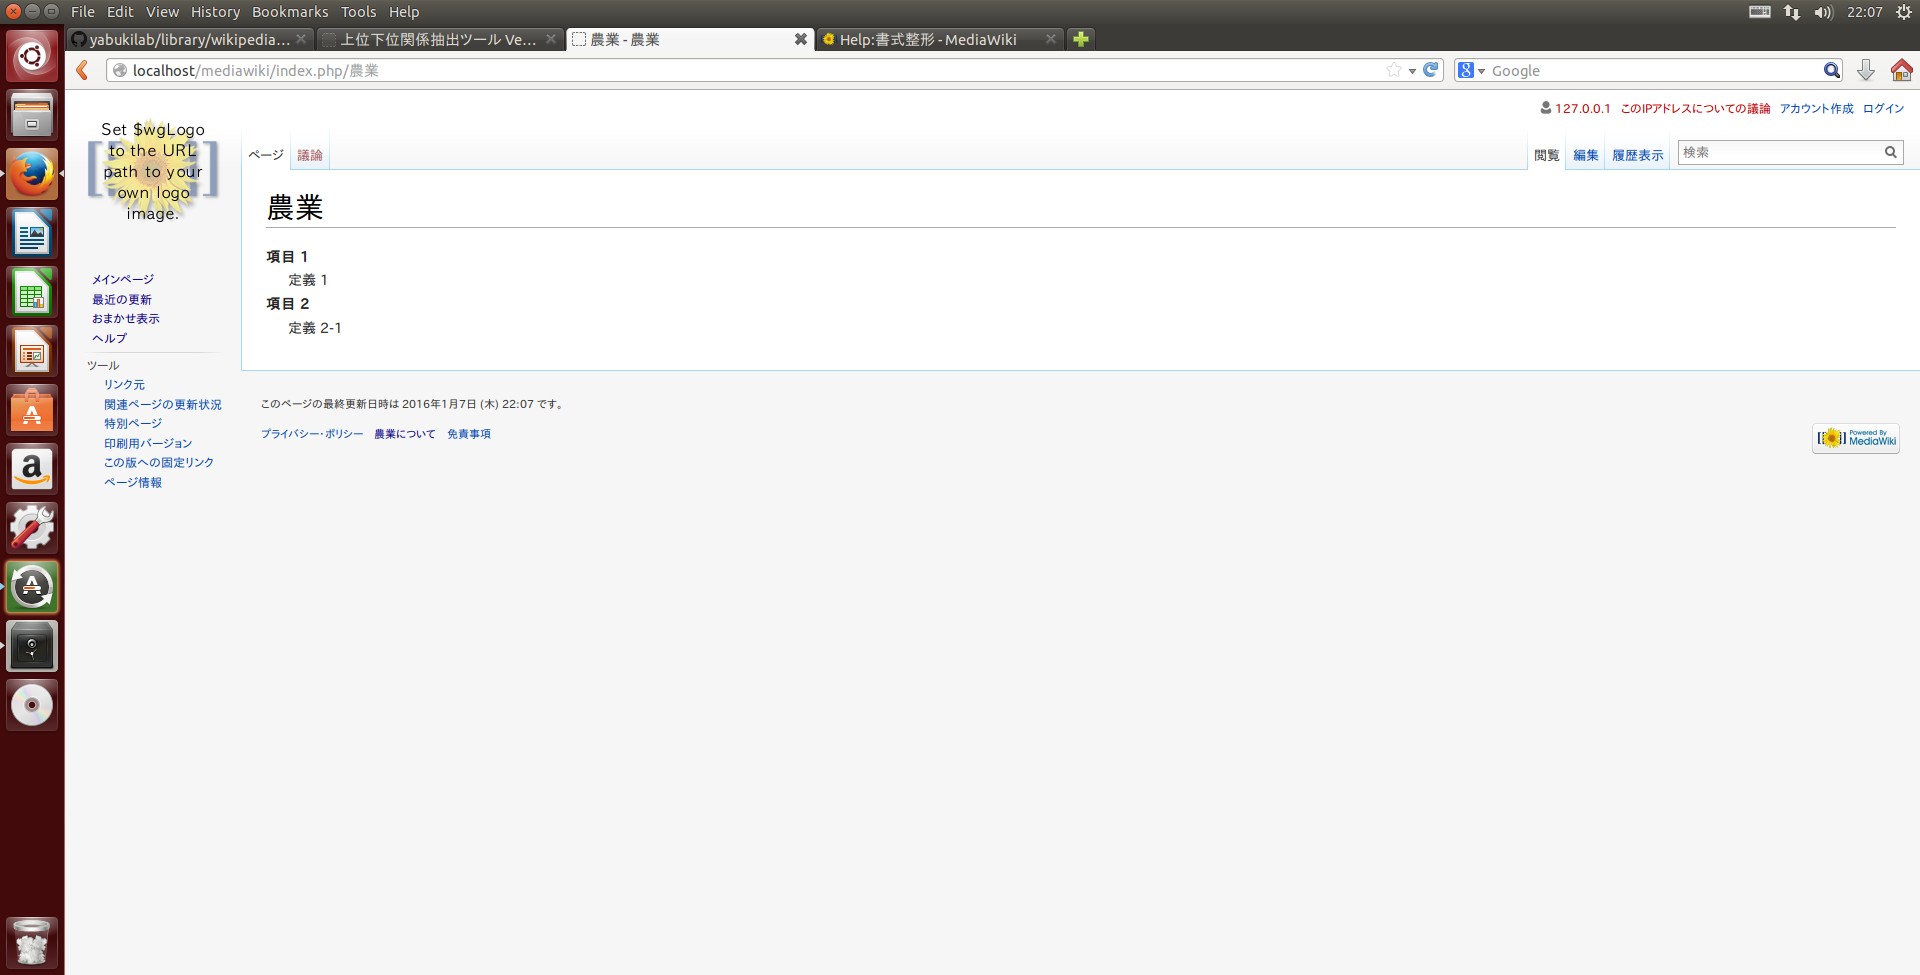
\includegraphics[width=14cm]{teigi}
\caption{定義リスト}\label{図}
\end{figure}

\subsection{挿入線}
挿入線とは,文字の下に線を引いた状態で表示したものである.挿入線は,「<ins>文字</ins>」もしくは「<u>下線</u>」で表示する.


%図の挿入
\begin{figure}[htb]
\centering
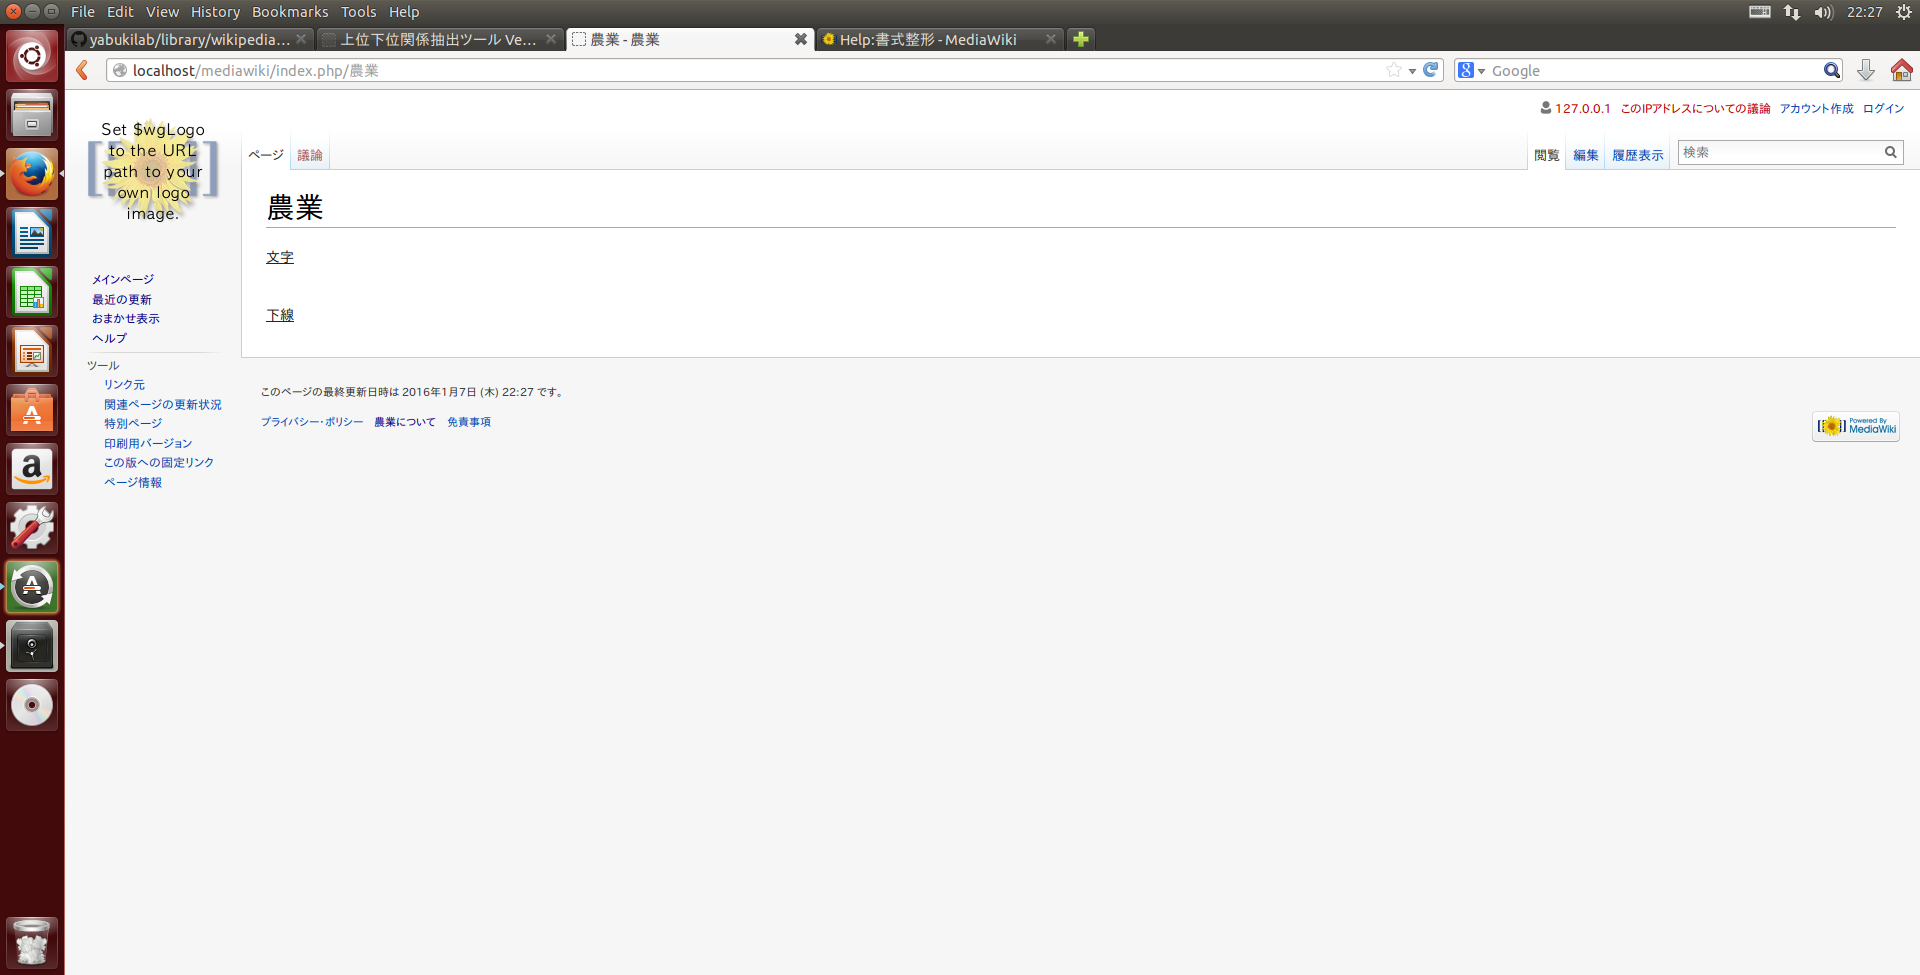
\includegraphics[width=14cm]{kasen}
\caption{挿入線}\label{図}
\end{figure}


\subsection{内部リンク}
内部リンクとは,同じウィキ内にあるページにリンクを張る方法である.同じウィキ内でリンクを張ることで,連携してより良い記事を書けるようになる.内部リンクは,「[[a]]」と表示する.記事が存在する場合は青で表示され,存在しない場合は,赤で表示される.


%図の挿入
\begin{figure}[htb]
\centering
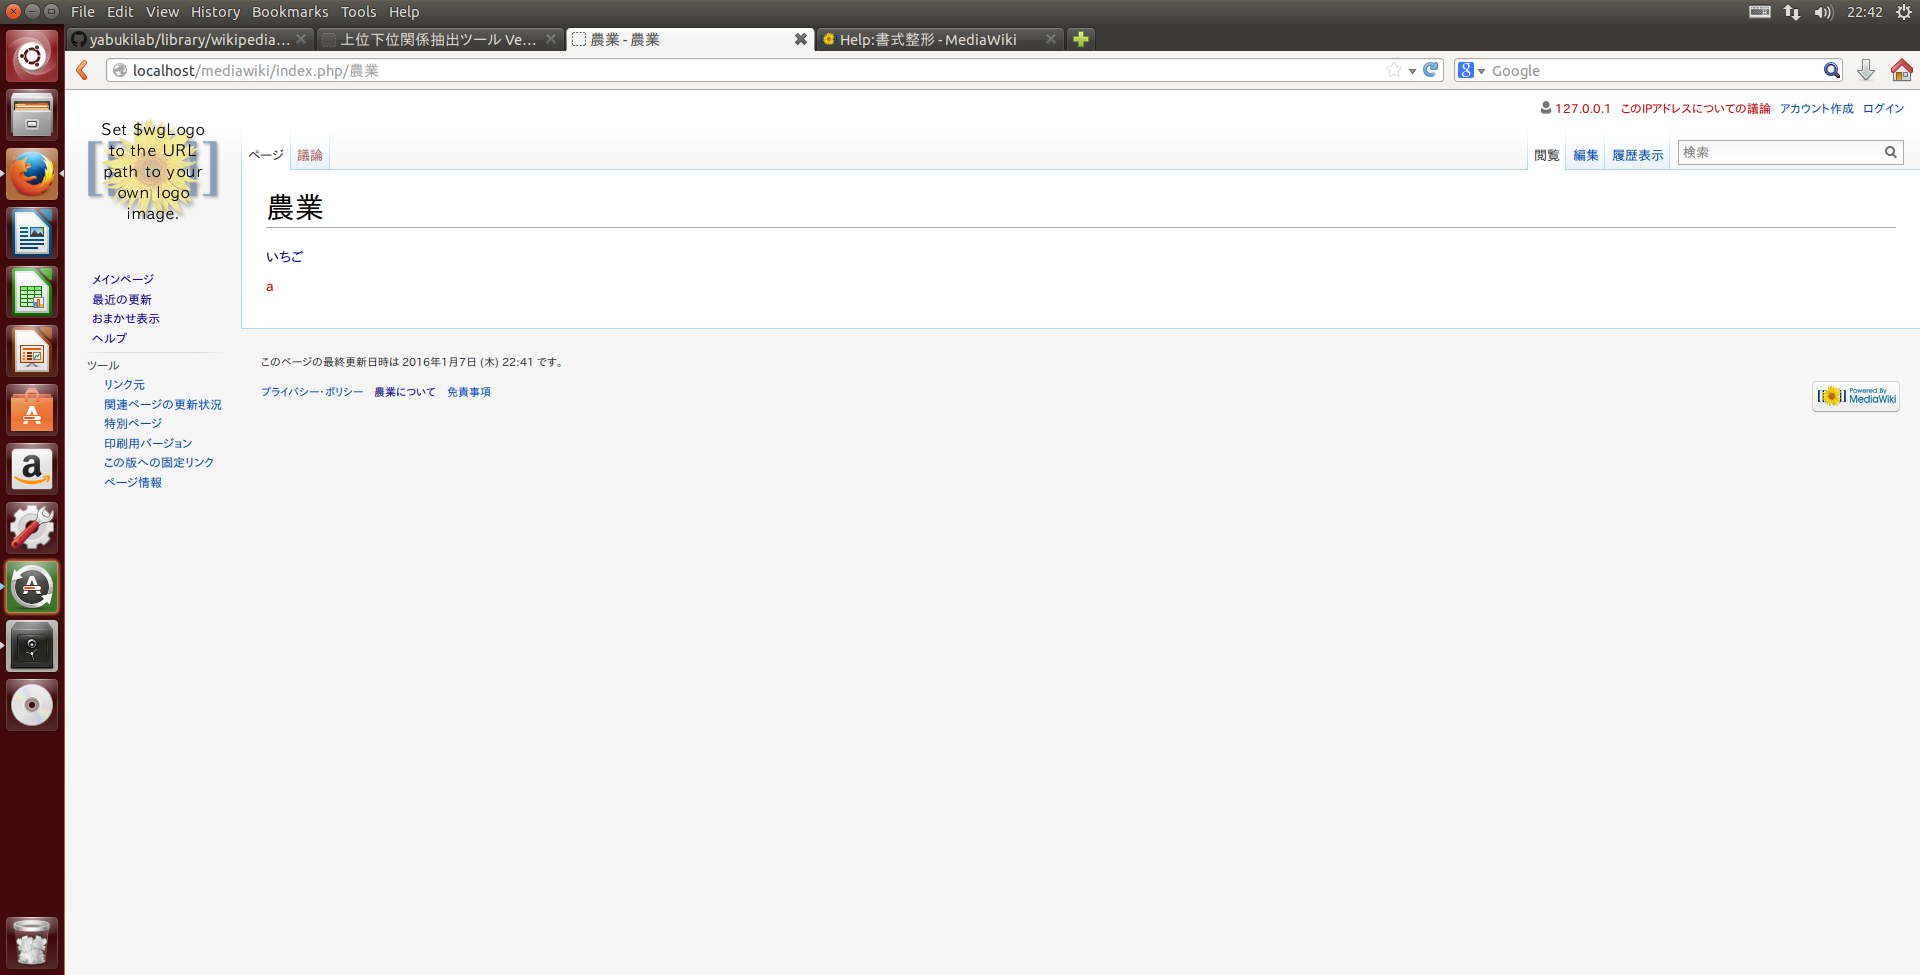
\includegraphics[width=14cm]{naibu}
\caption{内部リンク}\label{図}
\end{figure}

\subsection{外部リンク}
外部リンクとは,ウィキの外部のサイトにリンクを張る方法である.外部リンクは,参考文献などの外部へのリンクを張るときに使用する.外部リンクは,「[URL 名前]」と表示する.



%図の挿入
\begin{figure}[htb]
\centering
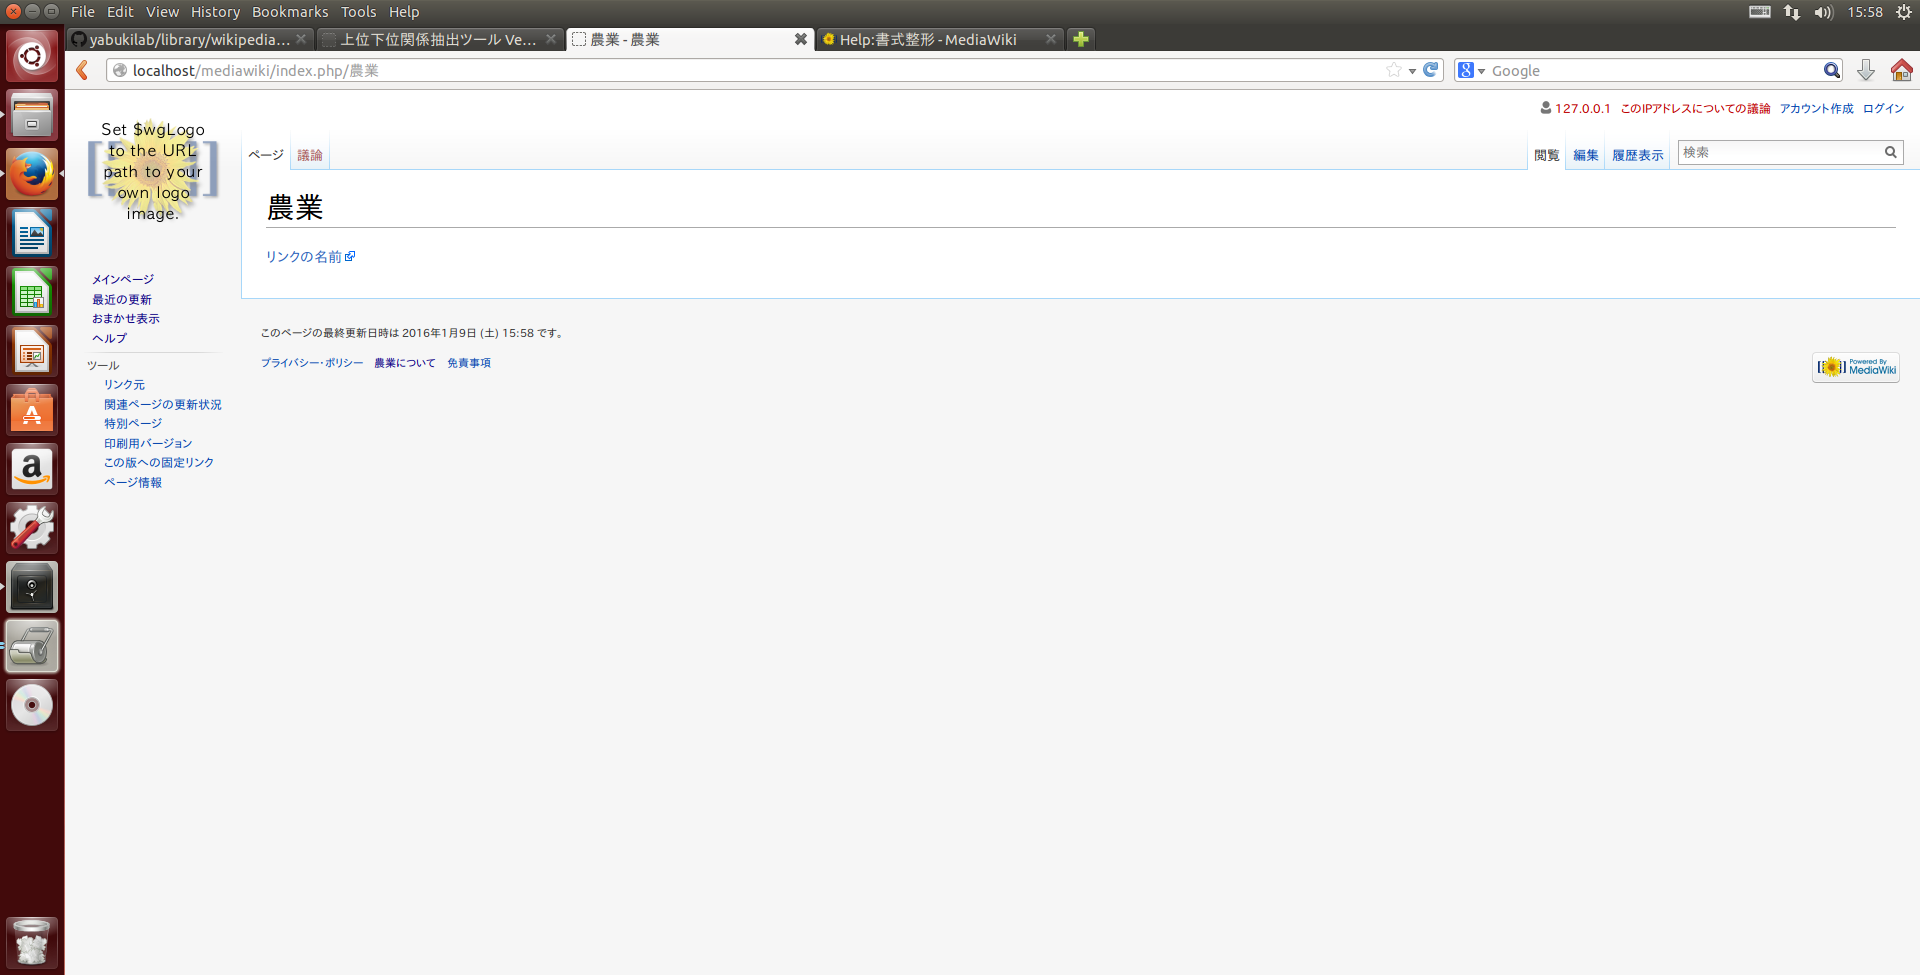
\includegraphics[width=14cm]{gaibu}
\caption{外部リンク}\label{図}
\end{figure}


\subsection{カテゴリ}
カテゴリとはウィキの機能の一つである.自動的に索引を生成し,プロジェクトの目次として使うことができる.カテゴリは,「[[Category:カテゴリ名]]」で表示される.




%図の挿入
\begin{figure}[htb]
\centering
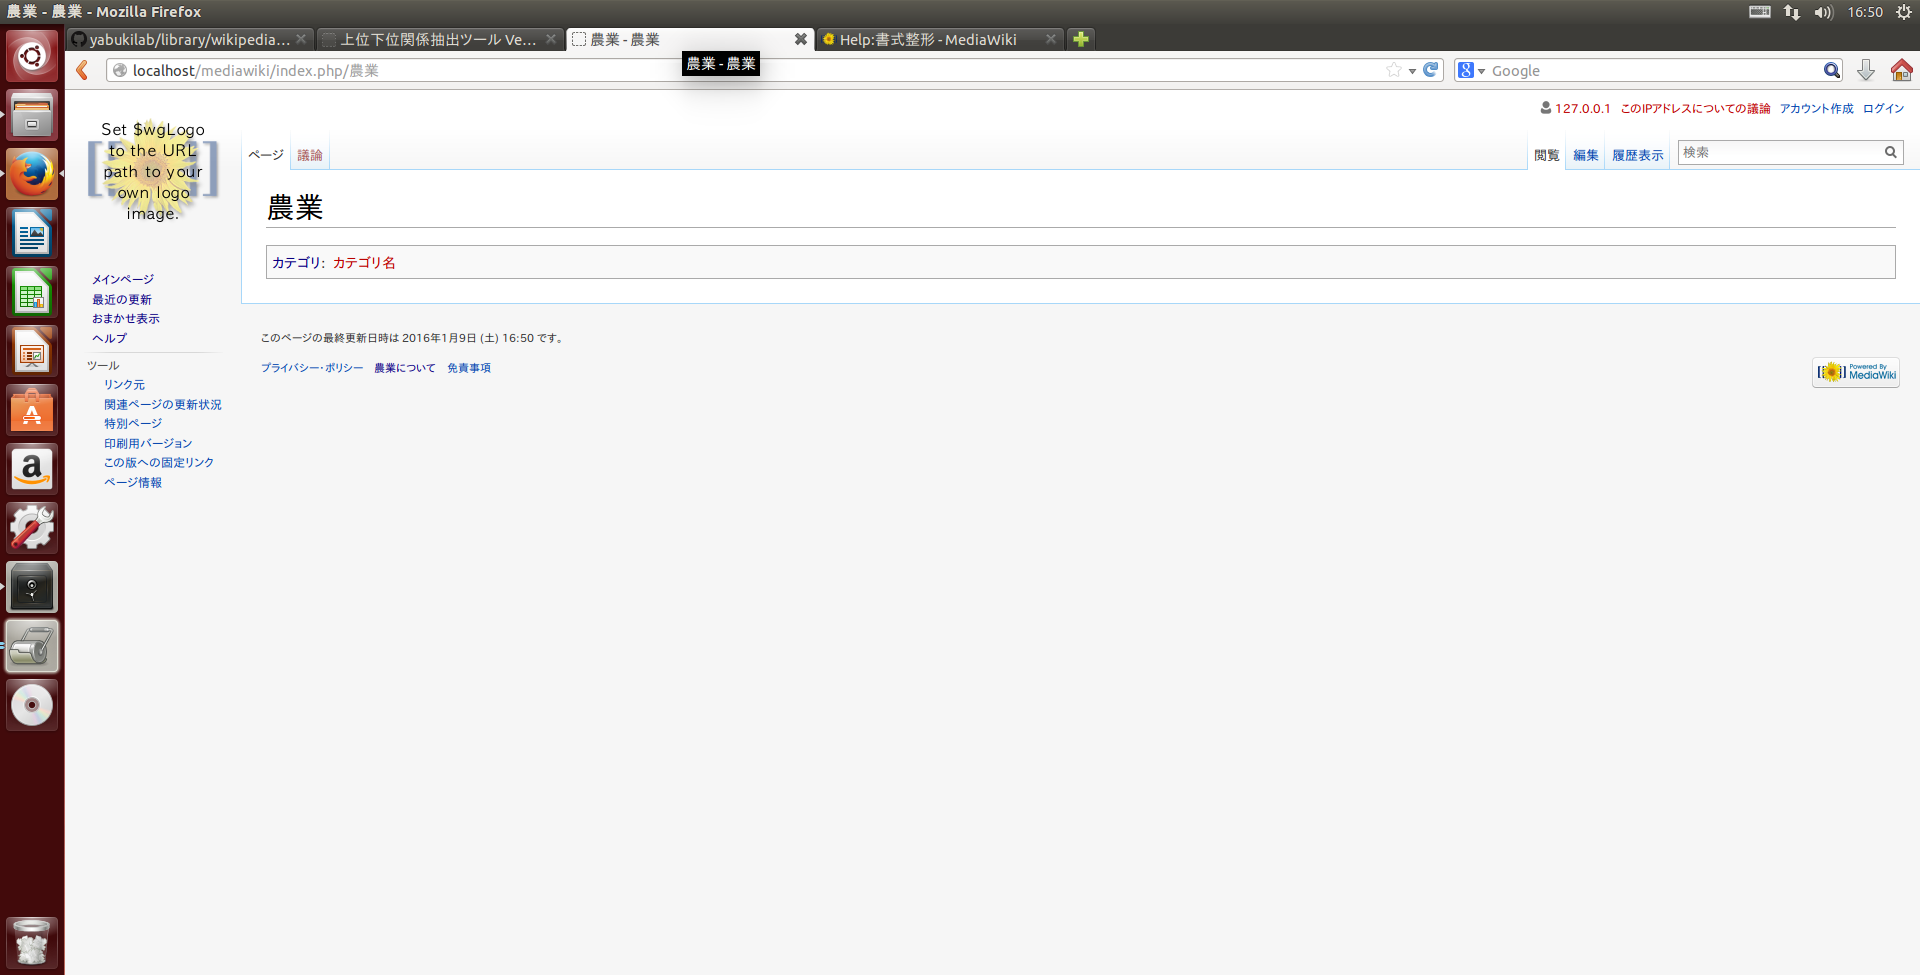
\includegraphics[width=14cm]{kategori}
\caption{カテゴリ}\label{図}
\end{figure}







\chapter{手法}
\section{本章の構成}
本章では研究方法と研究の事前準備と研究の手順を記載する.そして,実際に研究で使用したコードについても記載する.
\section{研究方法}

本研究の研究方法を説明する.本研究は,Mediawikiに情報を書き込み,それを解析した結果を以下の例のように表示することを目標とする.

\begin{figure}[!htb]
\centering
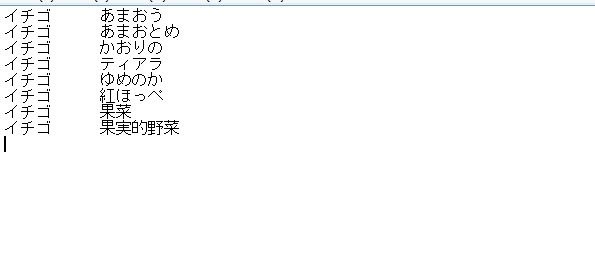
\includegraphics[width=18cm]{reidai.png}
\caption{解析目標}\label{kaiseki2}
\end{figure}

\begin{enumerate}
\item 情報の記載.
\item 解析.
\end{enumerate}
2つの作業を目標に達成するまで行う.




\subsection{事前準備}
本研究ではWindowsOSのコンピュータにとLinuxのディストリビューションであるUbuntuをVirtualBox上で動かしツールを使用して研究を行った.本項ではこのVirtualBoxと Ubuntu とツールの導入方法と使用方法を記す.

\subsection{VirtualBoxとは}
VirtualBoxとは,オープンソースの仮想化ソフトウェアの一つ.コンピュータ上に仮想的なコンピュータ(仮想マシン,VM:Virtual Machine)を構築し,その中でOSを起動して操作することができる.
VirtualBoxはコンピュータ上で直接動作している通常のOSにとってはアプリケーションソフトの一つであり,他のソフトと同じように起動することができる.起動すると仮想的なコンピュータが構築され,元のOSとは独立に別のOSを起動することができる.VirtualBoxが実行されているOSをホストOS,VirtualBox上で実行されているOSをゲストOSという.

ホストOSにはWindowsやMac OS X,Linux,Solarisなどを使用することができる.起動される仮想マシンはx86系あるいはx86-64系プロセッサで動作している(ように装う)ため,同プロセッサで起動するOSであれば基本的にはゲストOSとして起動することができる.

元は独立系のソフトウェア企業が開発・販売していた製品だったが,開発元がSun Microsystems社に買収され,その後同社がOracle社に買収されたため,Oracle社が開発元となり,正式名称も「Oracle VM VirtualBox」となった.また,VirtualBox本体はGPLに基いてオープンソースソフトウェアとして公開され,誰でも自由に入手・利用・改変・再配布などが行える.同社ではVirtualBoxに機能を追加するソフトウェアを製品として開発・販売している\cite{2016}.

\clearpage

\subsection{VirtualBoxの導入方法}
VirtualBoxの導入方法は以下のとおりである.
\begin{enumerate}
\item https://www.virtualbox.org/へアクセスしてDownloadsをクリックする.
\item 自分の環境にあったバージョンをダウンロードする.
\item ダウンロードしたら以下の画面が表示される.
\begin{figure}[hb]
\centering
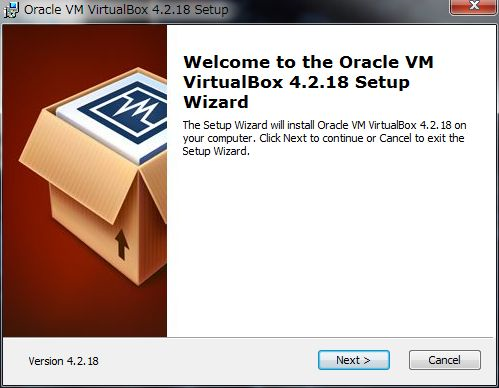
\includegraphics[width=10cm]{vm.png}
\caption{インストーラー画面}\label{vm.png}
\end{figure}
\item 設定をしてインストールする.
\item インストールが完了すると以下の画面が表示される.
\begin{figure}[hb]
\centering
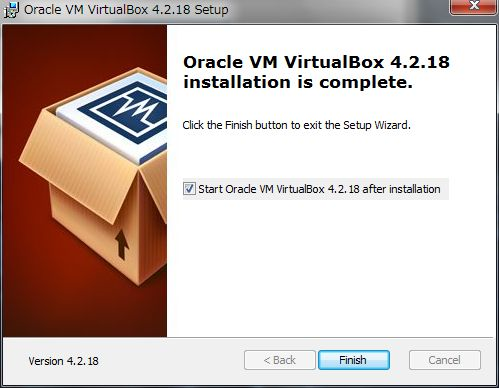
\includegraphics[width=10cm]{arsuto.png}
\caption{インストーラー終了画面}\label{arsuto.png}
\end{figure}
\end{enumerate}

以上がVirtualBoxの導入方法である\cite{2017}.



\subsection{仮想マシンの作成方法}
仮想マシンの作成方法はVirtualBoxを起動する.起動すると以下の画面が表示される.

\begin{figure}[hb]
\centering
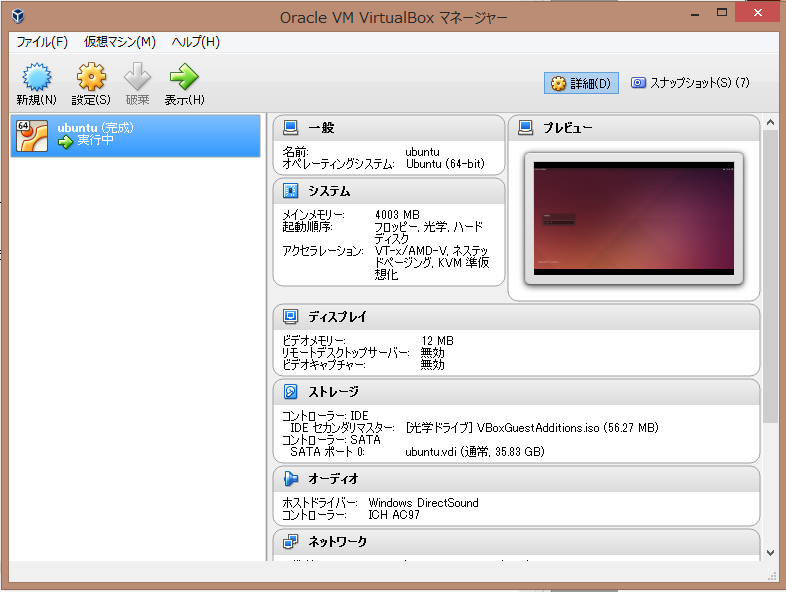
\includegraphics[width=10cm]{kasou.png}
\caption{VirtualBox起動画面}\label{kasou.png}
\end{figure}
新規作成を選択して,マシンの名前,メモリーサイズ,仮想ハードドライブの設定を行い作成する.本研究ではメモリを4ギガで行う.

\clearpage

\subsection{Ubuntuとは}
Ubuntu(ウブントゥ) とは、コミュニティ により開発されているオペレーティングシステムである.ラップトップ,デスクトップ,そしてサーバーに利用することができまる.Ubuntuには,家庭・学校・職場で必要とされるワープロやメールソフトから,サー バーソフトウェアやプログラミングツールまであらゆるソフトウェアが含まれている.

Ubuntu は現在,そして将来に渡って無償で提供されている.ライセンス料を支払う必要はない.Ubuntu をダウンロードすれば、友達や家族と,あるいは学校やビジネス に,完全に無料で利用できまる.

新しいデスクトップおよびサーバーを 6 ヶ月ごとにリリースすることを宣言している.これによりオープンソースの世界が提供する最新の優れたアプリケーションを常に利用できるようになっている.Quantal Quetzal 12.10 2012年10月18日 2014 年 4 月 

Ubuntu は,セキュリティに配慮して設計されている.デスクトップおよびサーバー の無償セキュリティアップデートが少なくとも 9 ヶ月間に渡って提供されいる.長期 サポート(LTS)版を利用すれば5 年間に渡りセキュリティアップデート提供される.もちろん,LTS 版を利用するために追加の費用は必要ありません.すべての人が無償とい う同じ条件で,私たちの精一杯の成果を利用することができます.Ubuntu を新しいバー ジョンにアップグレードする場合も,常に無償である.

Ubuntu のインストールイメージにはデスクトップ環境がひと通り含まれている.さ らに,オンラインでソフトウェアを追加することができる. 

グラフィカルインストーラにより,素早く簡単にインストールして使い始めることができる.標準的なインストールにかかる時間は 10〜20 分未満ででき,十分に高速な環境であればインストールが 5 分程度で終了することもある.
  
一度システムをインストールをすれば,インターネット,ドローイング,グラフィック ス,そしてゲームといったアプリケーションがすぐに使えるようになる.

Ubuntu サーバーでは,ユーザーがセットアップしたものだけが動作し,それ以外はイ ンストールされない\cite{ubuntu}.

\subsection{Ubuntuの意味}
Ubuntu は,アフリカの単語で他者への思いやりや皆があっての私といった意味を持つ.Linux ディストリビューションである Ubuntu は,Ubuntu の精神をソフトウェアの世界に届けようとしている\cite{ubuntu}.

\clearpage

\subsection{Ubuntuの日本環境}
Ubuntuは,できる限り多くの言語に対応すべく国際化が進められており,日本語での利用も可能である. Ubuntu Japanese Team では,Ubuntu 日本語サポートをより良いものとする活動を進められている.

しかしながら,他の言語環境に悪い影響を与えてしまう変更が必要であるなどの理由で,現段階ではオリジナルの Ubuntu に含めることが難しい修正が必要な場合もある. そこでJapanese Team では,現在のところ Ubuntu に 追加できていない修正を加えたパッケージ,および日本語環境に必要とされるパッケー ジを収録した Remix イメージと仮想ハードディスクイメージを作成・配布されている. 

この Japanese Team のパッケージを含むイメージを,オリジナルの Ubuntu と区別するために日本語 Remixや日本語 Remix 仮想ハードディスクイメージと呼ばれている\cite{ubuntu}.

\subsection{Ubuntuの特徴}
Ubuntu を使い,Web を閲覧したり,メールを読み書きしたり,文書や表計算をした り,画像を編集したり,その他さまざまなことができる.Ubuntu のデスクトップ CD には,早くて簡単なグラフィカルインストーラが搭載されている.一般的なコンピュータの場合,25 分以内でインストールが完了する.

主な特徴を以下にまとめる\cite{ubuntu}.


\begin{tabular}{|c|p{0.6\columnwidth}|}
 \hline
 シンプルなデスクトップ & デフォルトのデスクトップテーマは,目にやさしいものを使用している.\\\hline
    オフィスアプリケーション搭載 & オープンオフィスには,他のオフィススイートと似たユーザインタフェースと機能が備わっている.\\\hline
    ワープロ & ちょっとした手紙から書籍まで,さまざまな文書を編集することができる.\\\hline
    表計算 & 計算,分析,数表やグラフの作成のためのツール. \\\hline
    プレゼンテーション & 印象的なプレゼンテーションを作成するためのツール.\\\hline
    さまざまな形式のファイルを編集可能 & マイクロソフトオフィス,ワードなどのファイルを開いて編集することができる.\\\hline
    簡単で手軽なアップデ ート & アップデートは,タスクバーのアップデートエリアに表示され,このエリアで通知される.\\\hline
   ヘルプとサポート & メニューから[システム]-[ヘルプとサポ ート]を選択するか,https://help.ubuntu.com/にアクセスすることで公式ドキュメントを参照することができる.\\\hline
国際化とアクセシビリティ & Ubuntu にはフリーソフトウェアコミュニティが提供できる最大限の国際化とアクセシビリティ機構が含まれている. \\\hline
  システム要件 & Ubuntuは,x86 PC,64 ビットPCで利用することができる.少なくとも1ギガバイトのRAMと5ギガバイトのストレージスペースが必要である.\\\hline
\end{tabular}

\subsection{Ubuntuサーバーの特徴 }
Ubuntu サーバーは,堅牢なサーバーとして定評のあるDebianをベースとし,高い信頼 性とパフォーマンス,そして定期的なアップグレードを提供されている\cite{ubuntu}.

\begin{tabular}{|c|p{0.5\columnwidth}|}
 \hline
 統合されたセキュアなプラットホーム & プラットホームビジネスが成長するにつれ,ネットワークも大きくなる.
より多くのアプリケーションが必要となり,多くのサーバーが要求される.Ubuntu サーバーは,いくつかの共用設定をサポ ートし,一般的な Linux サーバの配置プロセスを単純化する. これにより,メール,Web,DNS,ファイル共有あるいはデー タベースといった一般的なインターネットサービスをうまくまとめたプラットフォームを,早く簡単に新しいサーバーにセットアップすることができる. Debianから受け継いだ鍵となる教訓は,デフォルトでセキュリティを保つこと.Ubuntu サーバーはインストール後どのポートも開いておらず,セキュアなサーバの構築に必要不可欠なソフトウェアのみが導入される. 
\\\hline
    自動LAMPインストー ルによるTCO削減 & Ubuntu サーバーのインストールは約15分以内で終了して, LAMP(Linux, Apache, MySQL, PHP)サーバが起動して利用可能な状態にできる.Ubuntuサーバーだけのこの機能は,インス トール時に利用することができる. LMAP オプションにより,LAMP の各コンポーネントを別々に インストールして設定する必要がなくなりる.各アプリケー
ションのインストールおよび設定方法を知っている方が数時 間かかる作業を自動的に行うことができる.LAMP オ プションを使えば,十分なセキュリティ,インストール時間の削減,設定ミスリスクの軽減を実現することができ,その結果 コストの削減につながる.\\\hline
\end{tabular}

\begin{tabular}{|c|p{0.5\columnwidth}|}
 \hline
  ワークステーションをアップグレードするコストの削減 & Ubuntu サーバーにはLTSP(Linux Terminal Server Project)を利用したシンクライアントサポートが含まれている.最新版である LTSP-5 により,単純なインストールと簡単なメンテナンス が提供されている.すべてのデータはサーバーに蓄積され,個々のワークステーションをアップデートし,セキュリティを 保つよりも大幅にコストを削減することができる.Ubuntuのシンクライアントサポートによる利点には以下のようなものがある.
 \par 簡単な管理:一つのシステムからすべてのクライアントを管理できる.新しいソフトウェアのインストール,それらの設定変更,サーバー上のあたらしいバージョンへのアップグレード,そしてすべてのクライアントをすぐに最新の状態にすることさえ可能である.全てのクライアントのバックアップを 1 箇所でとることもできる.
 \par 完全に自動化されたインストールとセットアップ:シンクライアントサーバーをインストールするのは,デスクトップシステムのインストールと同じぐらい簡単である.一度インストールを終えれば,サーバー上で管理作業を行うことなく新しいクライアントを加えることができる.
 \par 共通リソースにより TCO 低減:ハイパワーなデスクトップワークステーションを何台も電源を入れ,一日中アイドル状態にしておくとコストがかさんでしまう.ハイパワーなサーバーと,低コストのシンクライアントを使えば,パフォーマンスが良い上コストも節約できる.さらにパフォーマンスを上げたいならば,サーバー一台をアップグレードすれば,クライアントのパフォーマンスも改善される.
 \par 高速な障害復旧:クライアントシステムが故障しても,他のシステムを使って仕事を継続することができる.特別な設定は必要なく,すべてのユーザーデータと設定は保持されている.\\\hline
\end{tabular}


\subsection{Ubuntuの導入方法}
 Ubuntuの導入方法は以下の通りである.
\begin{enumerate}
\item 仮想化ソフトを使用し,Ubuntuのインストールを行うための仮想マシンを作成する.
\item UbuntuのISOイメージのダウンロードを行う.http://www.ubuntulinux.jp/へアクセスし日本語remixのUbuntuのダウンロードを行う.
\item 作成した仮想マシン上にUbuntuのインストールを行う.インストールが完了すると以下の図9-1 Ubuntu14.04デスクトップ画面のような画面が表示される. 
\end{enumerate}


%図の挿入
\begin{figure}[htb]
\centering

\includegraphics[width=14cm]{ubuntugamen}
\caption{Ubuntu14.04デスクトップ画面}\label{図}
\end{figure}

\subsection{端末の使用方法}
本研究では Ubuntu 上での操作には主にアプリケーションのアクセサリ内にある「端末」を使用した.この端末上ではコマンドを実行することによってソフトウェアのインストールやプログラムの実行といった Ubuntu の操作をすべて行うことができる. 

端末を開いたウィンドウ内には以下のような表示がされるので,$に続けてコマンドを入力し[Enter]キーを押し実行させる. 

ユーザー名@ホスト名:カレント(作業)ディレクトリ\$

Linux で使用する主なコマンドは以下の表にまとめた.
 
\begin{table}[htb]
  \begin{center}
  \begin{tabular}{|l|c|} \hline
    コマンド & 機能 \\ \hline \hline
    ls & ファイルの一覧表示 \\  \hline
    cp & ファイルのコピー \\  \hline
    mv & ファイルの移動,ファイル名の変更 \\ \hline
    rm & ファイルの削除 \\  \hline
    pwd & カレントディレクトリの表示 \\  \hline
    cd & カレントディレクトリの変更 \\ \hline
    cat & ファイルの内容を表示 \\  \hline
   python & pythonプログラムの起動  \\  \hline
   sh & bashプログラムの起動 \\  \hline
  mysql & ユーザー名とパスワードを同時に記載することでmysqlが起動 \\ \hline
  curl & プロトコルを用いてデータを通信するコマンドライン ツール \\  \hline
 echo & 因数に与えられた文字列を表示する \\  \hline
   > & ファイルに出力する \\  \hline
 chmod &ファイルやディレクトリのアクセス権を変更する \\  \hline
 grep & 文字列を検索する \\  \hline
  \end{tabular}
  \end{center}
\caption{コマンド表}
\end{table}

\clearpage

\subsection{Mediawikiを使用する理由}
Mediawikiは,ネットワークにつながる環境があればどこからでも編集することができる.さらにMediawikiは,プログラミング言語などより独自の書式があり,自然言語が自動で処理してくれるため編集しやすい.そのためMediawikiは,農家の生産者が作った新しい品種や新しい名称などを自分で登録できるので使用する.

\subsection{Mediawikiの導入方法}
MediawikiのUbuntuでの導入方法を説明する.まず,端末で以下のように記入する.説明を加えて記述する.

管理者権限があることを確認する.
{\small
\begin{verbatim}
sudo ls
\end{verbatim}}


作業ディレクトリに移動する.
{\small
\begin{verbatim}
cd
mkdir tmp
cd tmp
\end{verbatim}}

MySQLの管理者パスワードを`pass`とする.
{\small
\begin{verbatim}
echo 'mysql-server mysql-server/root_password password pass' | sudo debconf-set-selections
echo 'mysql-server mysql-server/root_password_again password pass' | sudo debconf-set-selections
\end{verbatim}}
 phpMyAdminをインストールする準備をする.
{\small
\begin{verbatim}
echo 'phpmyadmin phpmyadmin/reconfigure-webserver multiselect apache2' | sudo debconf-set-selections
echo 'phpmyadmin phpmyadmin/dbconfig-install boolean true' | sudo debconf-set-selections
echo 'phpmyadmin phpmyadmin/mysql/admin-pass password pass' | sudo debconf-set-selections
echo 'phpmyadmin phpmyadmin/mysql/app-pass password pass' | sudo debconf-set-selections
echo 'phpmyadmin phpmyadmin/app-password-confirm password pass' | sudo debconf-set-selections
\end{verbatim}}

必要なソフトウェアをインストールする.
{\small
\begin{verbatim}
sudo apt-get update
sudo apt-get install -y mysql-server phpmyadmin
\end{verbatim}}

MediaWikiをダウンロードし,展開する.
{\small
\begin{verbatim}
wget https://releases.wikimedia.org/mediawiki/1.25/mediawiki-1.25.2.tar.gz
tar zxf mediawiki-1.25.2.tar.gz
sudo mv mediawiki-1.25.2 /var/www/html/mediawiki
\end{verbatim}}

設定画面を開く.
{\small
\begin{verbatim}
firefox http://localhost/mediawiki/ &
\end{verbatim}}
設定画面を開くと,以下の画面が表示される.
\begin{figure}[ht]
\centering
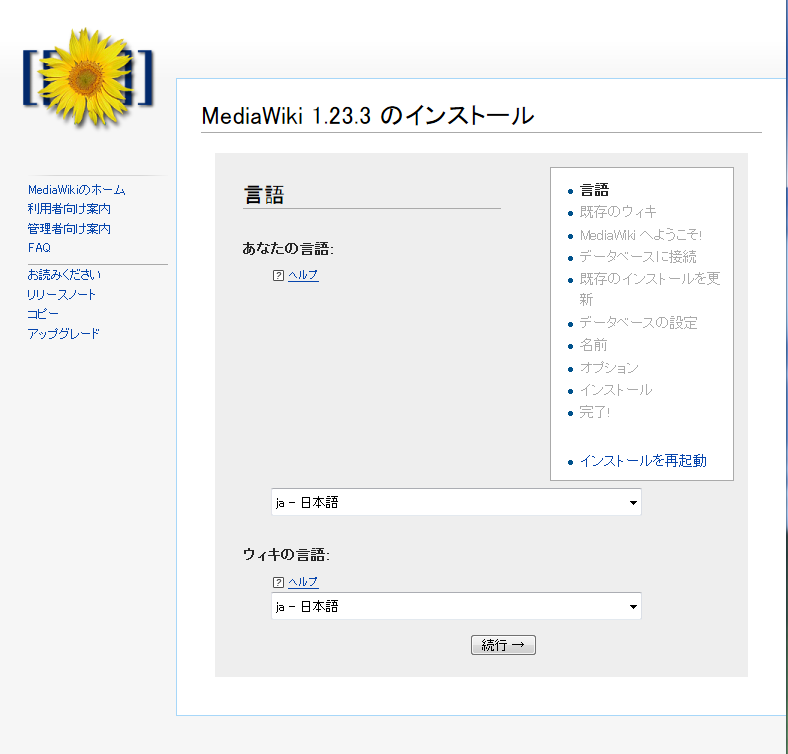
\includegraphics[width=14cm]{settei}
\caption{Mediawikiセットアップ画面}\label{settei}
\end{figure}

Mediawikiの設定は,以下の通り設定した.
\begin{enumerate}
\item .データベースのパスワード欄に,先に設定したパスワードpassを入力する.
\item .ウィキ名欄に農業という名前を入力する.
\item .管理アカウントの管理者名をadmin,パスワードをpassとする.
\end{enumerate}
以上の設定を終えたら「もう飽きてしまったので、とにかくウィキをインストールしてください。」を選び, LocalSettings.phpというファイルを保存する.


LocalSettings.phpのファイルを移動させる.
{\small
\begin{verbatim}
sudo mv ~/ダウンロード/LocalSettings.php /var/www/html/mediawiki/
\end{verbatim}}
以上でMediawikiが使えるようになる.成功した場合は,以下の画面になる.

\begin{figure}[ht]
\centering
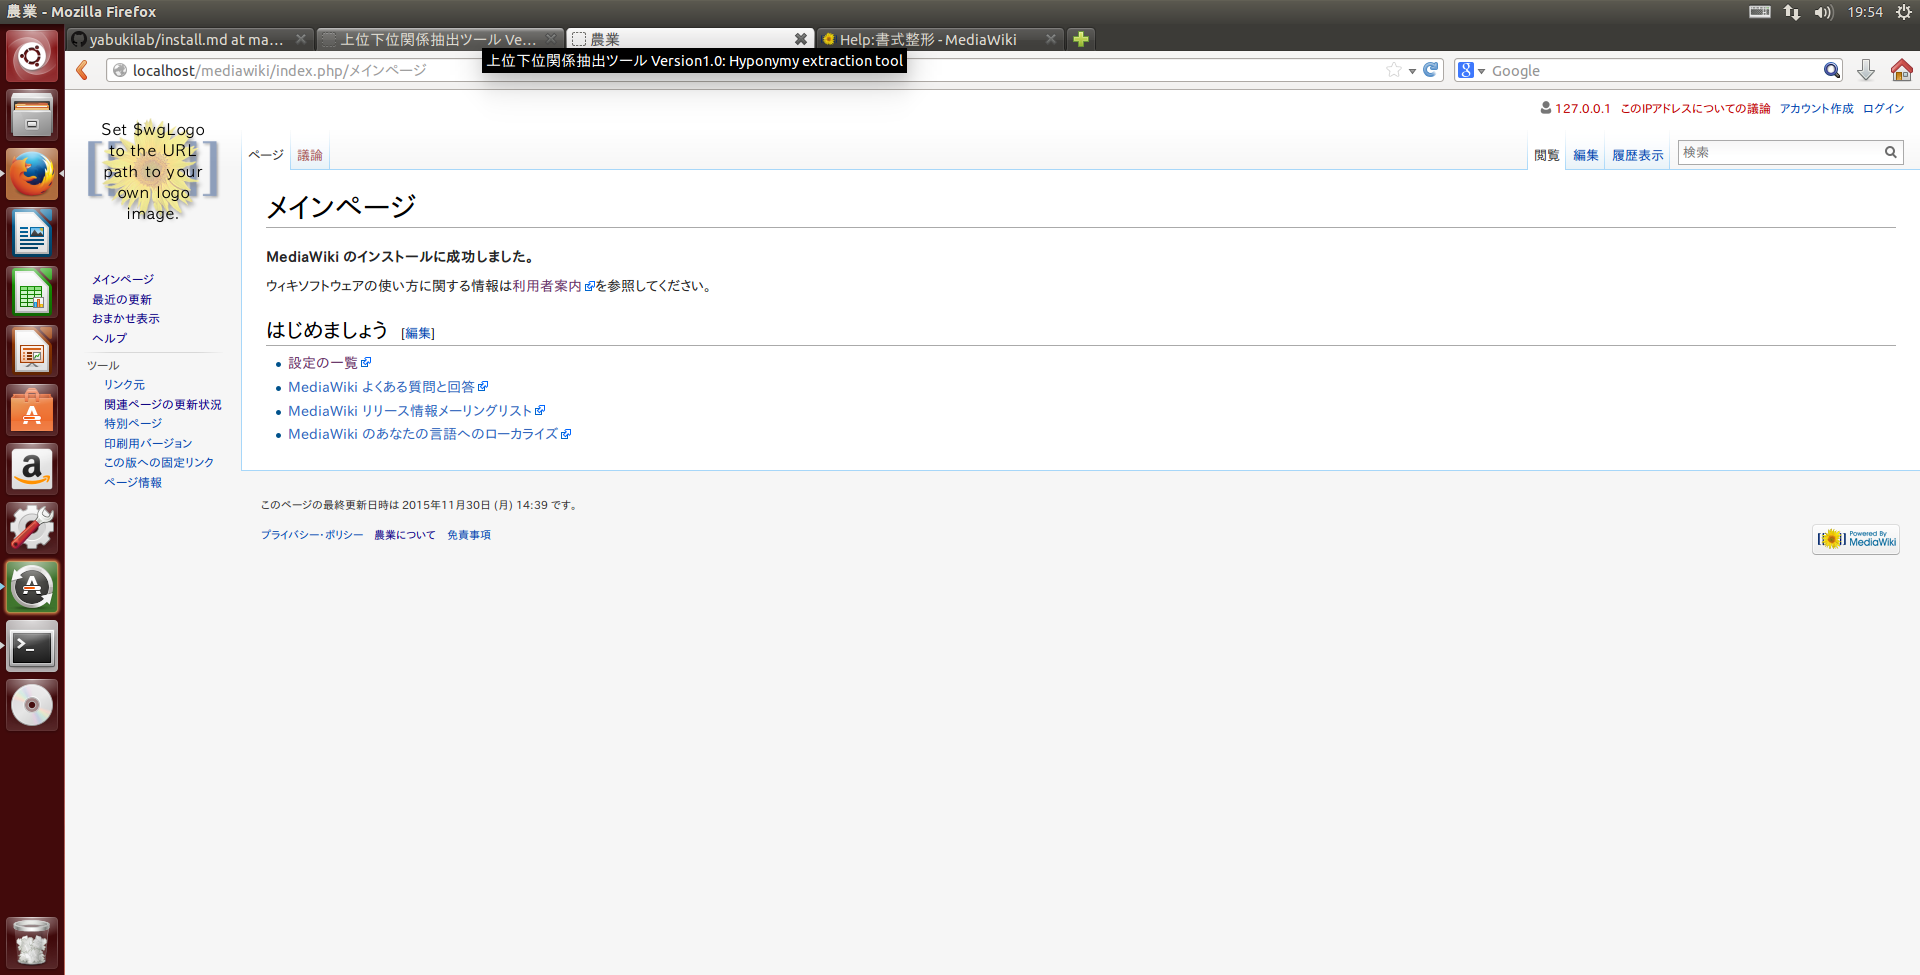
\includegraphics[width=15cm]{mein}
\caption{Mediawikiメインページ}\label{mein}
\end{figure}

失敗や最初からやり直すときは以下のコードを使う.

データベースを削除する.
{\small
\begin{verbatim}
echo 'drop database my_wiki;' | mysql -uroot -ppass
\end{verbatim}}

ファイルを削除する.
{\small
\begin{verbatim}
sudo rm -r /var/www/html/mediawiki
\end{verbatim}}

\subsection{上位下位関係抽出ツール導入方法}
上位下位関係抽出ツールの導入方法を説明する.

作業ディレクトリに移動する.
{\small
\begin{verbatim}
cd
mkdir tmp
\end{verbatim}}

Rubyをインストールする.
{\small
\begin{verbatim}
sudo apt-get update
sudo apt-get -y install software-properties-common
sudo apt-add-repository ppa:brightbox/ruby-ng
\end{verbatim}}

Ruby 1.8をインストールする.
{\small
\begin{verbatim}
sudo apt-get update
sudo apt-get -y install ruby-switch ruby1.8 rubygems1.8 ruby1.8-dev
sudo ruby-switch --set ruby1.8
\end{verbatim}}

バージョン1.8が使えることを確認する
{\small
\begin{verbatim}
ruby -v
\end{verbatim}}

次のように表示されれば成功
{\small
\begin{verbatim}
ruby 1.8.7 (2015-04-14 MBARI 8/0x6770 on patchlevel 375) [x86_64-linux], MBARI 0x6770, Ruby Enterprise Edition2012.02
\end{verbatim}}

Mecabをインストールする.
{\small
\begin{verbatim}
sudo apt-get -y install mecab mecab-ipadic-utf8 libmecab-dev
\end{verbatim}}

RubyからMeCabを使えるようにする.
{\small
\begin{verbatim}
cd ~/tmp
wget -O mecab-ruby-0.994.tar.gz https://mecab.googlecode.com/files/mecab-ruby-0.994.tar.gz
tar zxf mecab-ruby-0.994.tar.gz
cd mecab-ruby-0.994
gem build mecab-ruby.gemspec
sudo gem install mecab-ruby
\end{verbatim}}

 test.rb の3行目に以下のように require 'rubygems' を追記して ruby test.rb で動作を確認する.
\begin{figure}[hb]
\centering
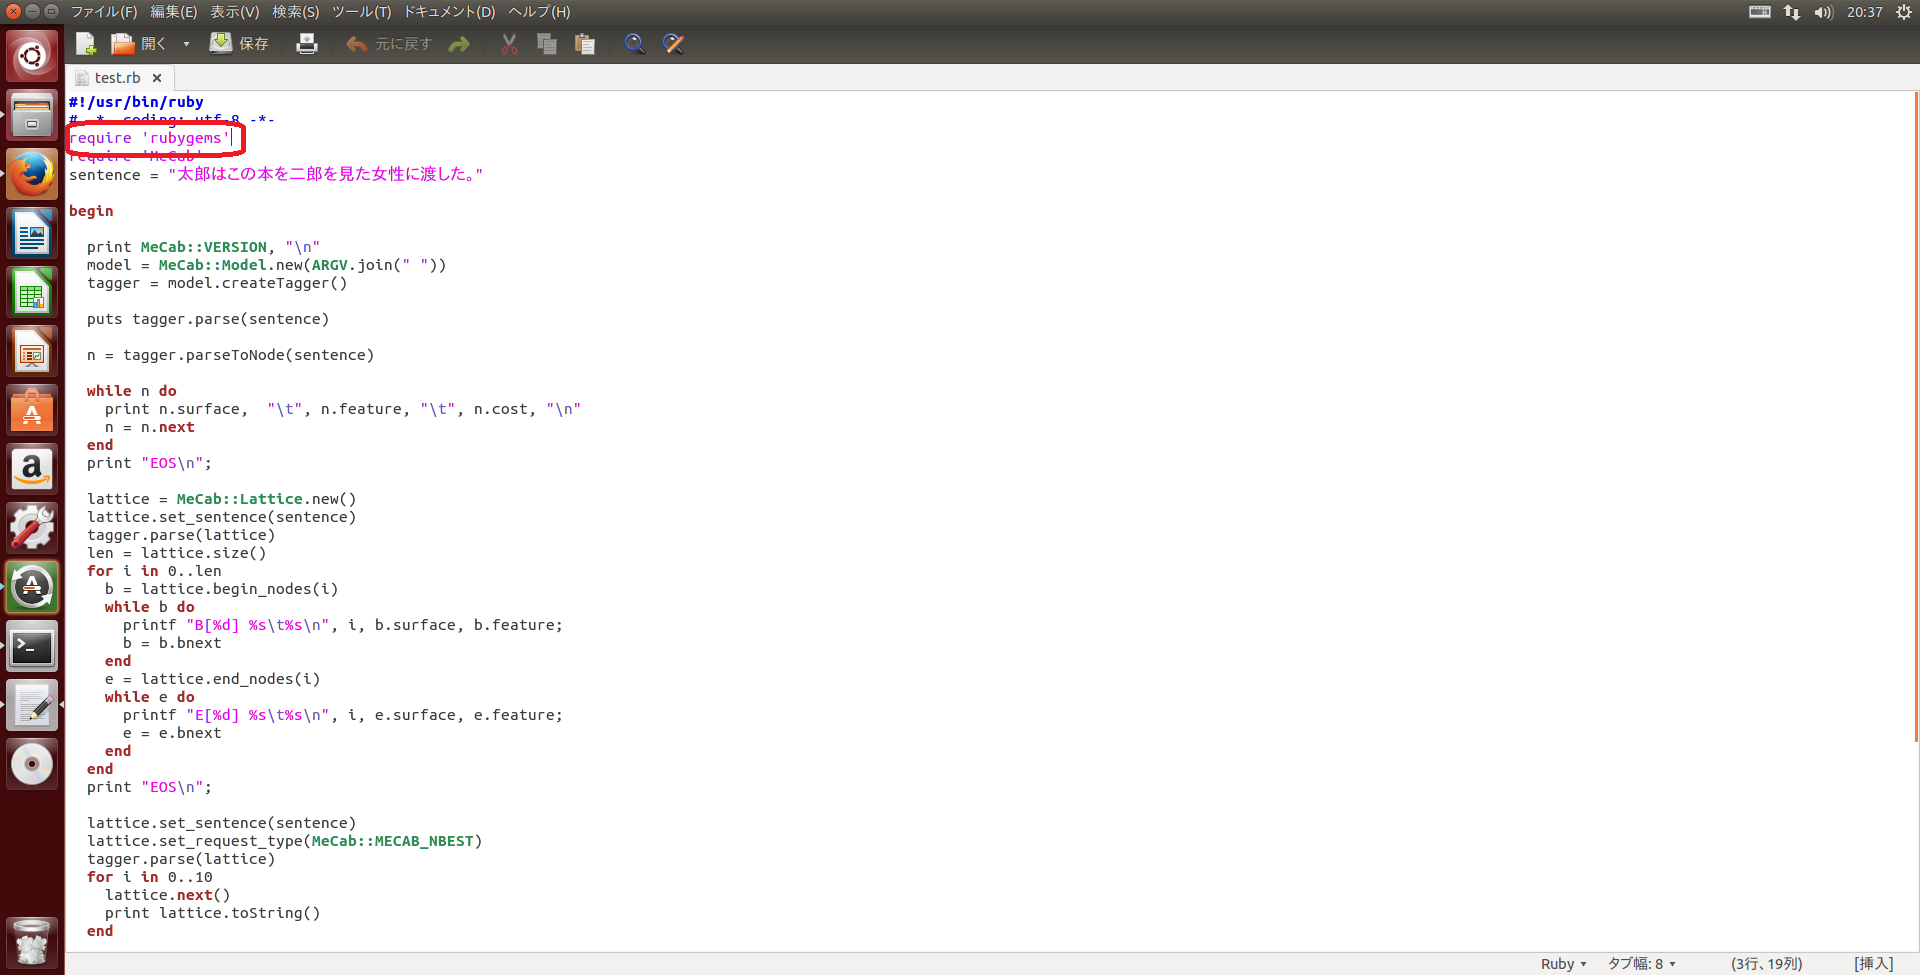
\includegraphics[width=15cm]{testrb}
\caption{test.rbファイル画面}\label{testrb}
\end{figure}

Peccoをダウンロードする.
{\small
\begin{verbatim}
cd ~/tmp
wget http://www.tkl.iis.u-tokyo.ac.jp/~ynaga/pecco/pecco-latest.tar.gz
tar zxf pecco-latest.tar.gz
cd pecco-XXXX-XX-XX #場合による。「pecco」まで入力してTABキーで補完すればよい。
./configure
sudo make install
\end{verbatim}}

Hyponymyをダウンロードする.
{\small
\begin{verbatim}
cd ~/tmp
wget -O ex-hyponymy-1.0.tar.gz https://alaginrc.nict.go.jp/hyponymy/cgi-bin/dl.1.0.cgi
tar zxf ex-hyponymy-1.0.tar.gz
cd ex-hyponymy-1.0
\end{verbatim}}

パッチを当てる.
{\small
\begin{verbatim}
wget http://www.tkl.iis.u-tokyo.ac.jp/~ynaga/pecco/ex-hyponymy-1.0-pecco.patch
patch -p0 < ex-hyponymy-1.0-pecco.patch
\end{verbatim}}

part.rb の require 'Cut' の前の行に require 'rubygems' という1行を以下のように追記する.
\begin{figure}[hb]
\centering
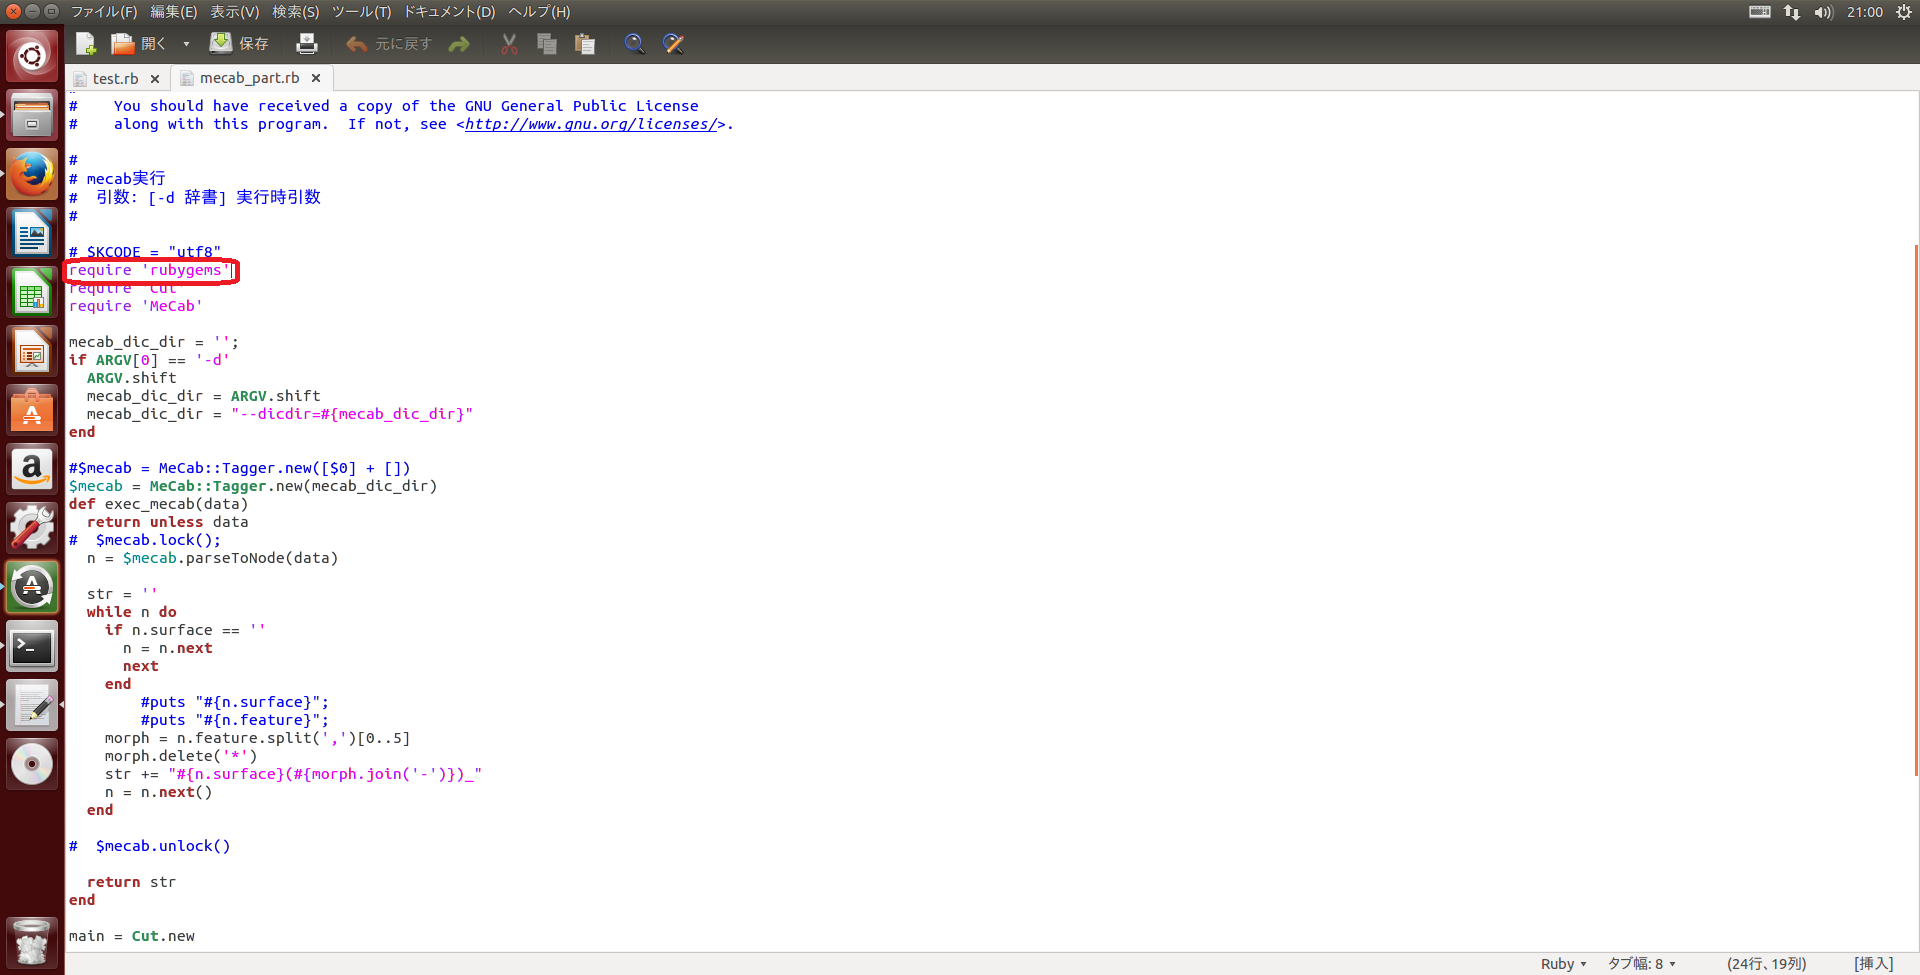
\includegraphics[width=15cm]{require}
\caption{mecabのpart.rbファイル画面}\label{require}
\end{figure}

チェックする.
{\small
\begin{verbatim}
gedit script/lib/mecab_part.rb &
\end{verbatim}}

以上が研究環境の事前準備である.

\section{上位下位関係抽出ツールについて}
上位下位関係抽出ツールについてとその使い方を記述する.

\subsection{上位下位関係抽出ツールとは}
上位下位関係抽出ツールとは,Wikipediaダンプデータ(XMLファイル)から機械学習を使って上位下位関係となる用語ペアを数百万対のオーダーで抽出できるツールである. 上位下位関係とは,"XはYの一種(一つ)である"と言えるXとYの関係を言う. Xのことを下位語,Yのことを上位語と呼び,別の言い方をすると,上位下位関係は「上位概念ー下位概念」または「概念ーインスタンス(具体例)」の関係を持つ語の対となる. 抽出できる上位下位関係の単語対の総体は,単語の分類,シソーラスと見なすこともできる. 
\clearpage
また,本ツールの出力する上位語,下位語はいわゆる「単語」にとどまらず「志摩市のスポーツイベント」のように詳細な意味を表す複合的な言語表現を含む.

 上位下位関係抽出ツールは,知る限り,日本語に関する上位下位関係を世界最大規模で抽出できる. 2010年6月24日バージョンのWikipediaに対して適用した場合,精度90%程度で約600万対の上位下位関係が抽出される. この約600万対の上位下位関係は,上位語異なり数約20万語,下位語異なり数約245万語をカバーしている. \cite{Hyponymy}

上位下位関係となる用語ペアの抽出処理では,Wikipediaのページから以下の3種類を情報源として上位下位関係候補を抽出し,各候補が上位下位関係であるか否かを統計的に判定している.

\begin{itemize}
 \item hierarchy :箇条書きなどの階層構造から上位下位関係の候補を抽出.
\end{itemize}

\begin{figure}[hb]
\centering
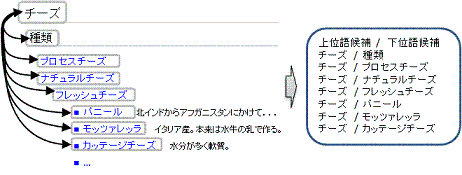
\includegraphics[width=13cm]{hierarchy}
\caption{hierarchy例}\label{hierarchy}
\end{figure}

\begin{itemize}
 \item definition :最初の文(定義文)から上位下位関係の候補を抽出(「~とは,….」などを利用).
\end{itemize}

\begin{figure}[hb]
\centering
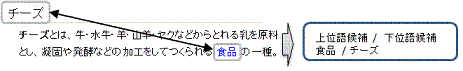
\includegraphics[width=13cm]{definition}
\caption{definition例}\label{definition}
\end{figure}

\begin{itemize}
 \item category :category tagにある単語から上位下位関係の候補を抽出.
\end{itemize}

\clearpage

\begin{figure}[hb]
\centering
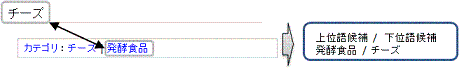
\includegraphics[width=13cm]{category}
\caption{category例}\label{category}
\end{figure}

\section{上位下位関係抽出ツールの使用理由}
上位下位関係抽出ツールを使用する理由は,関連用語を上位と下位に分け,wikiから抽出できるからである.wikiから抽出できるため,Mediawikiの使用方法で記述した通り,図9.10のようにできるからである.

\begin{figure}[hb]
\centering
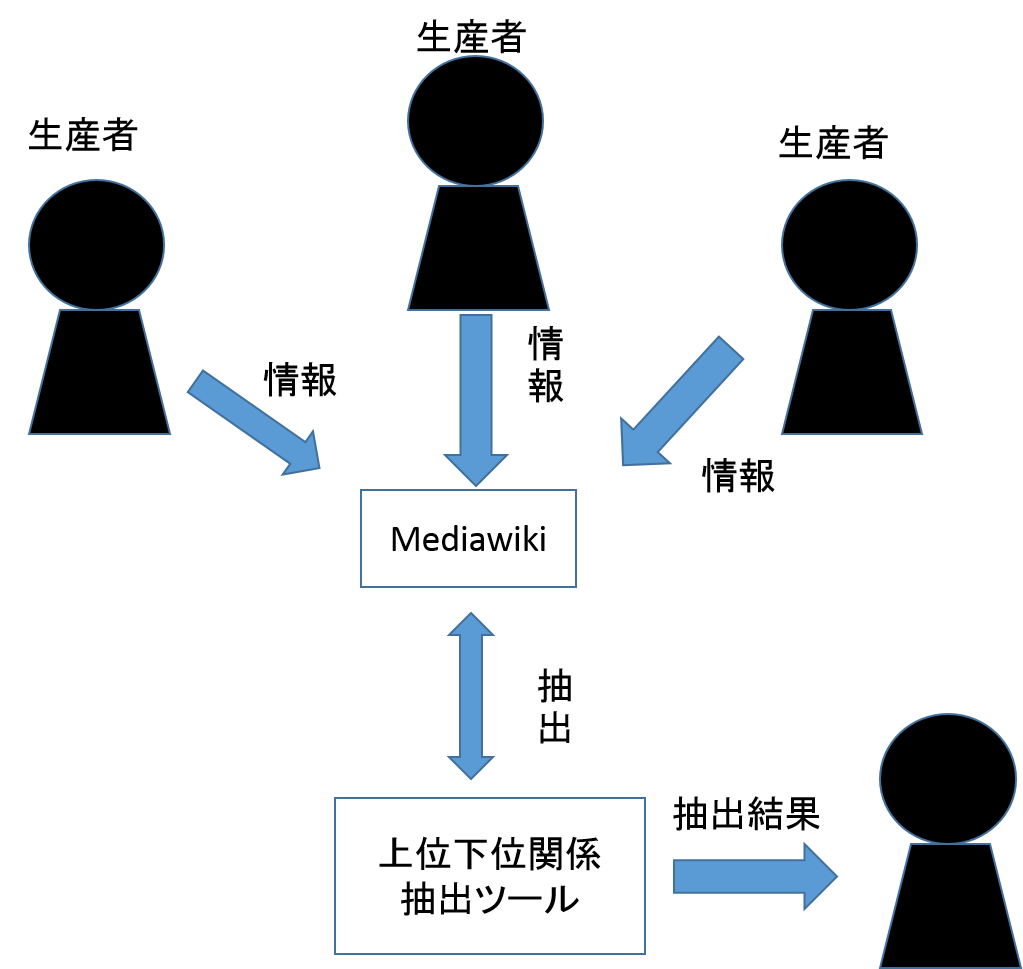
\includegraphics[width=13cm]{zyouikai.png}
\caption{全体例}\label{zyouikai.png}
\end{figure}


\subsection{テスト準備}
Mediawikiを使った上位下位関係抽出ツールでテストを行う.そのために準備するものを記述する.なおテストデータは,ハクサイと鍋料理の情報を使用する.

最初にMediawikiにハクサイと鍋料理のページを作り,Wikipediaの記事をMediawikiに記載する.
Mediawikiに記載したハクサイと鍋料理のページは以下のものである.

\begin{figure}[!htb]
\centering
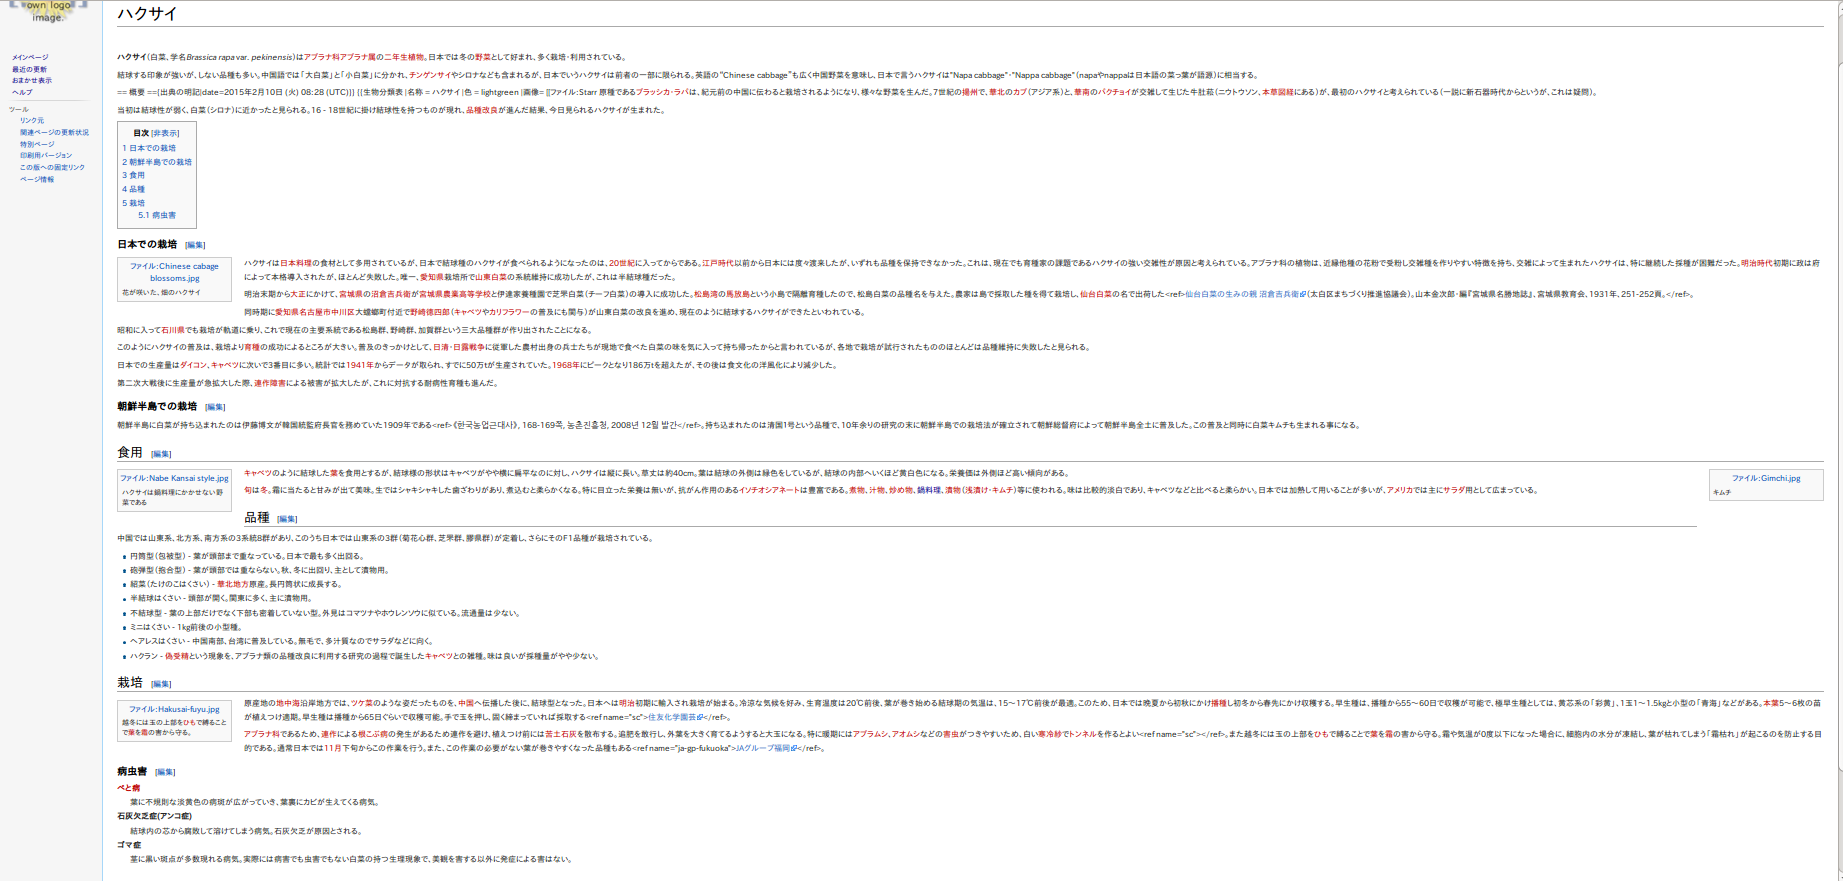
\includegraphics[width=18cm]{hakusai}
\caption{ハクサイ画面}\label{hakusai}
\end{figure}

\begin{figure}[!htb]
\centering
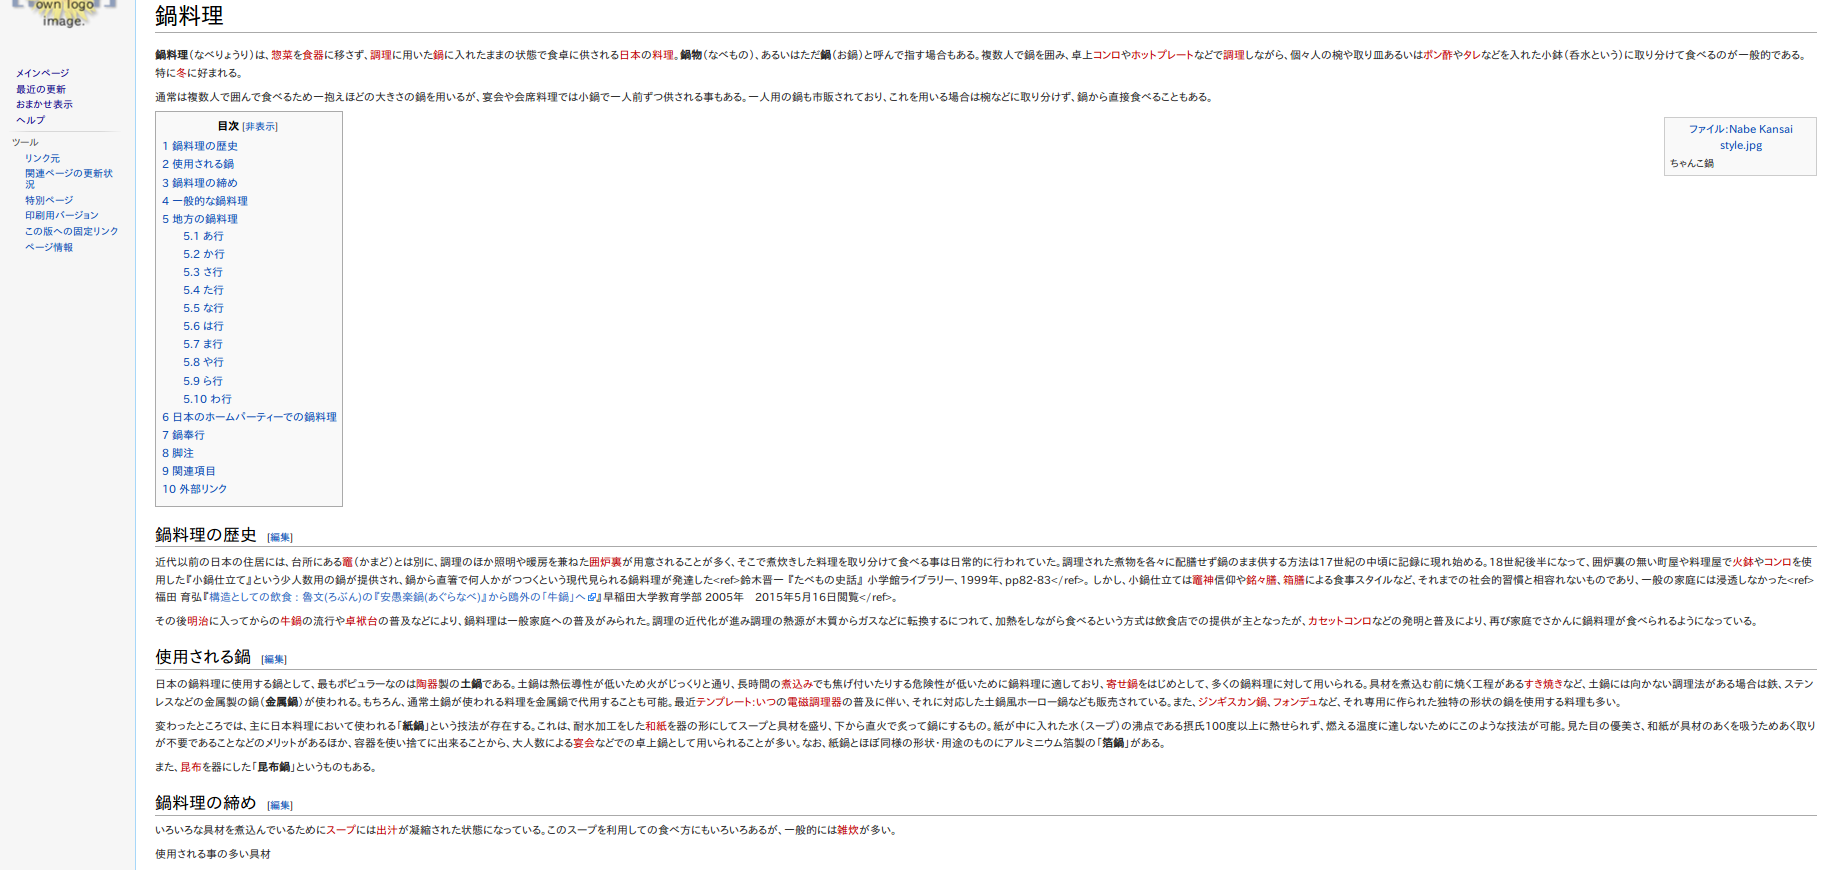
\includegraphics[width=18cm]{nabe}
\caption{鍋料理画面1}\label{nabe}
\end{figure}

\begin{figure}[!htb]
\centering
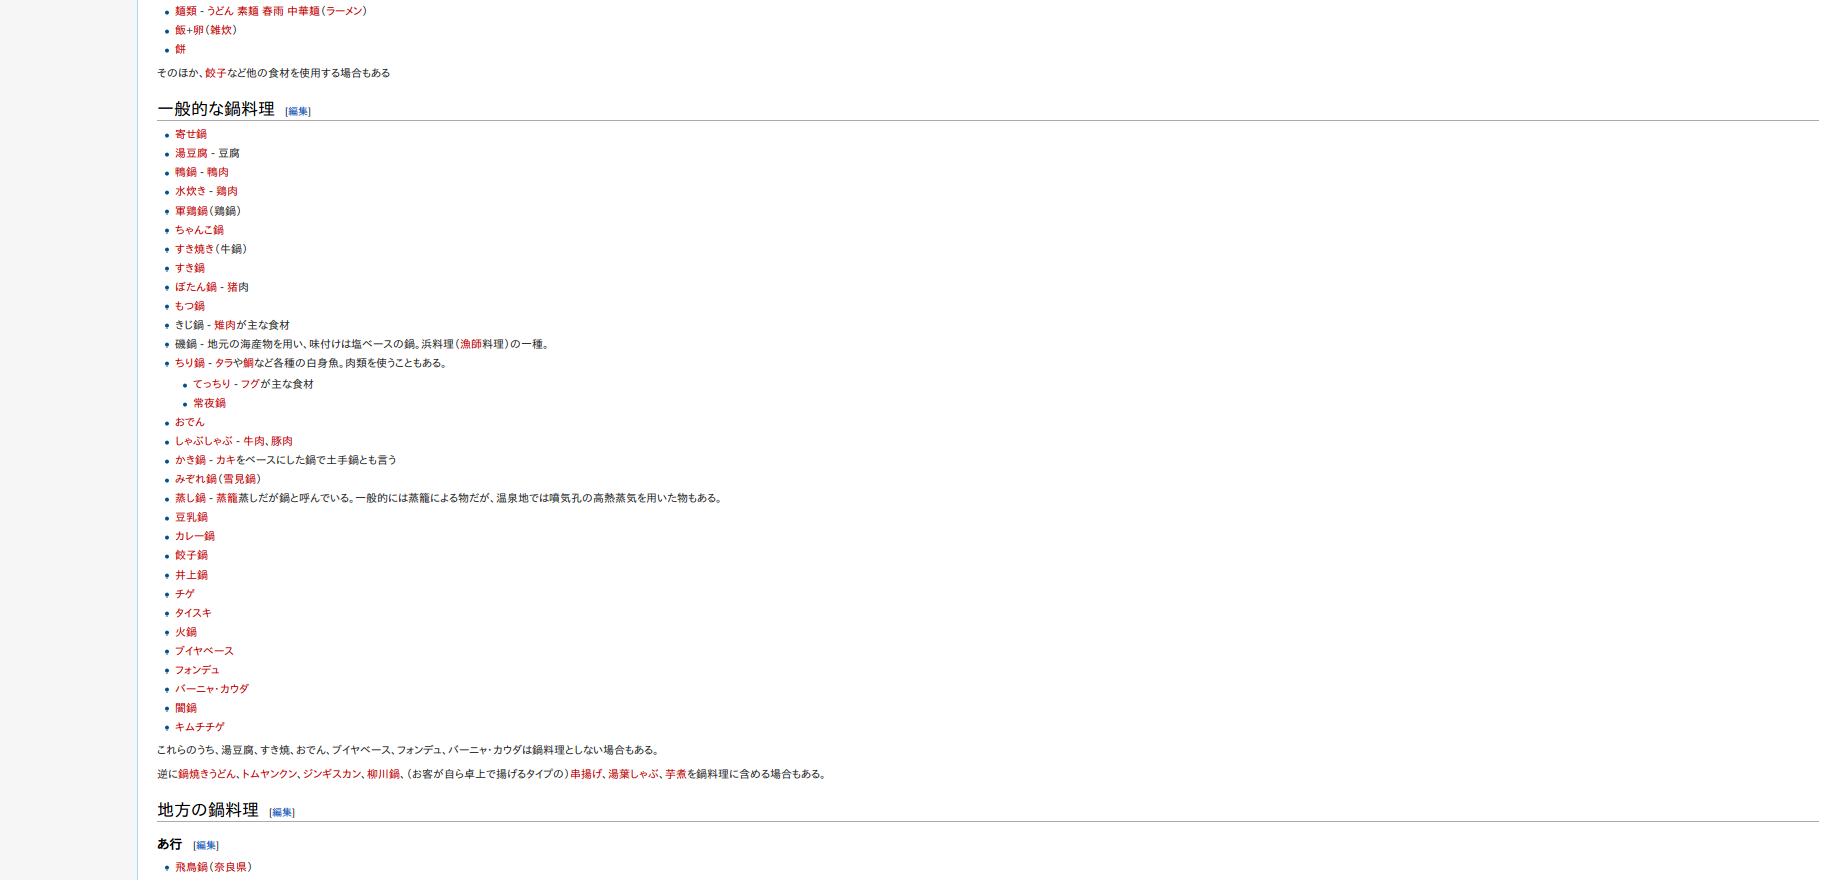
\includegraphics[width=18cm]{nabe2}
\caption{鍋料理画面2}\label{nabe2}
\end{figure}

\begin{figure}[!htb]
\centering
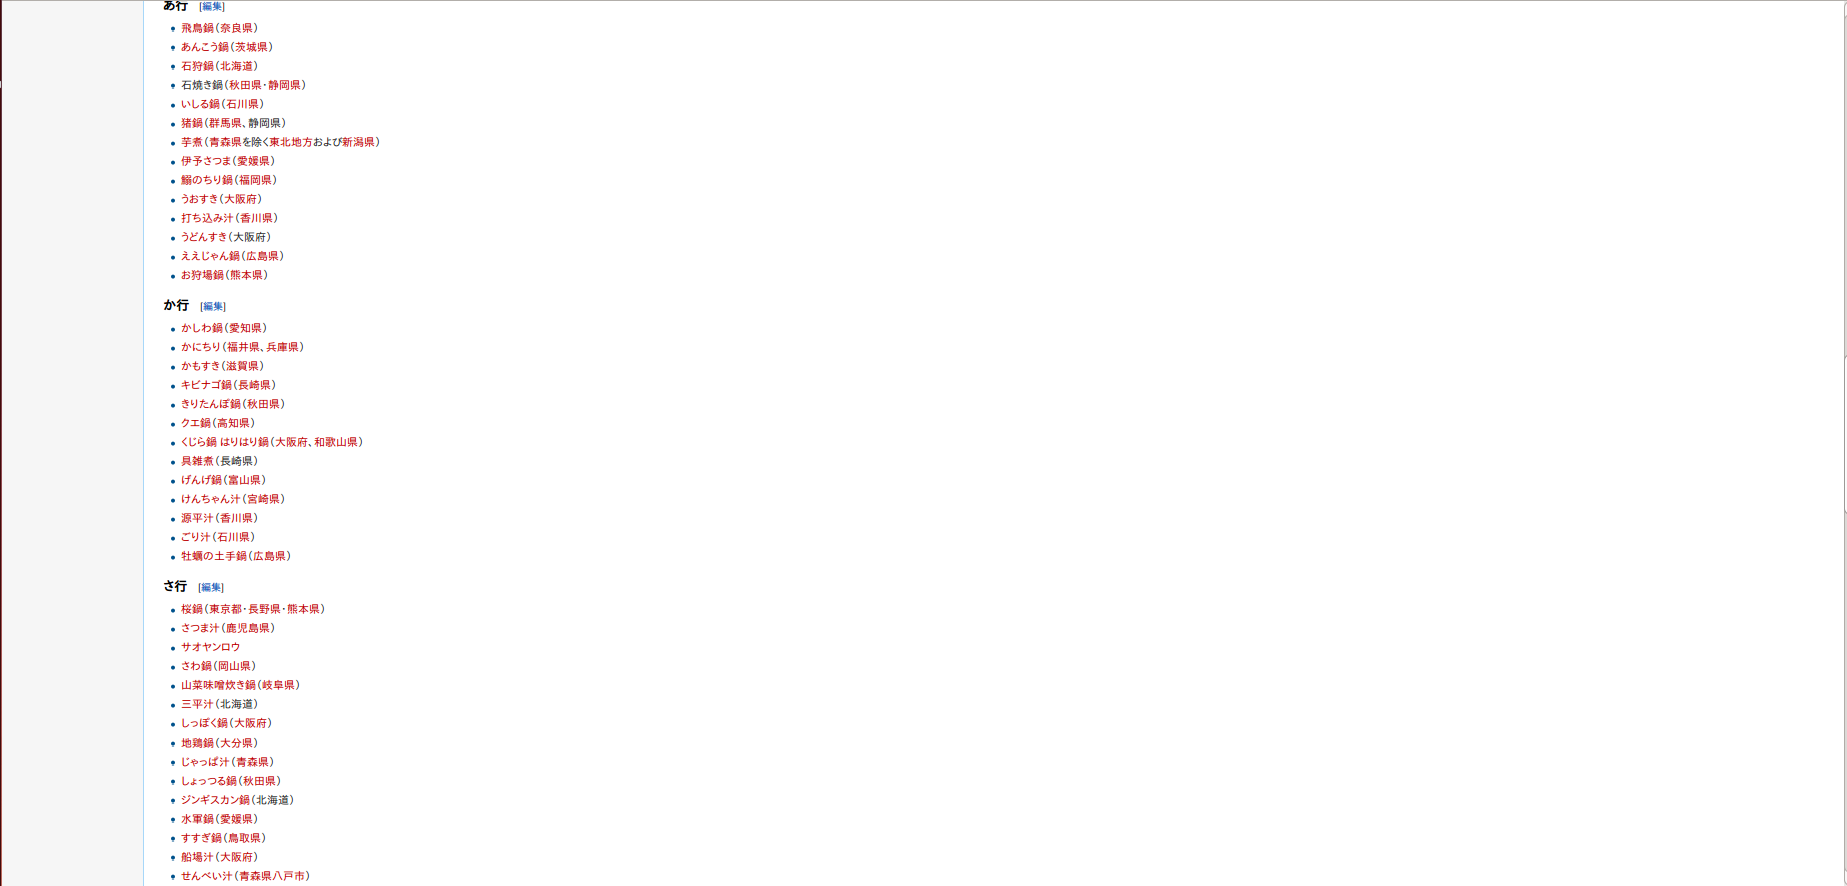
\includegraphics[width=18cm]{nabe3}
\caption{鍋料理画面3}\label{nabe3}
\end{figure}

\begin{figure}[!htb]
\centering
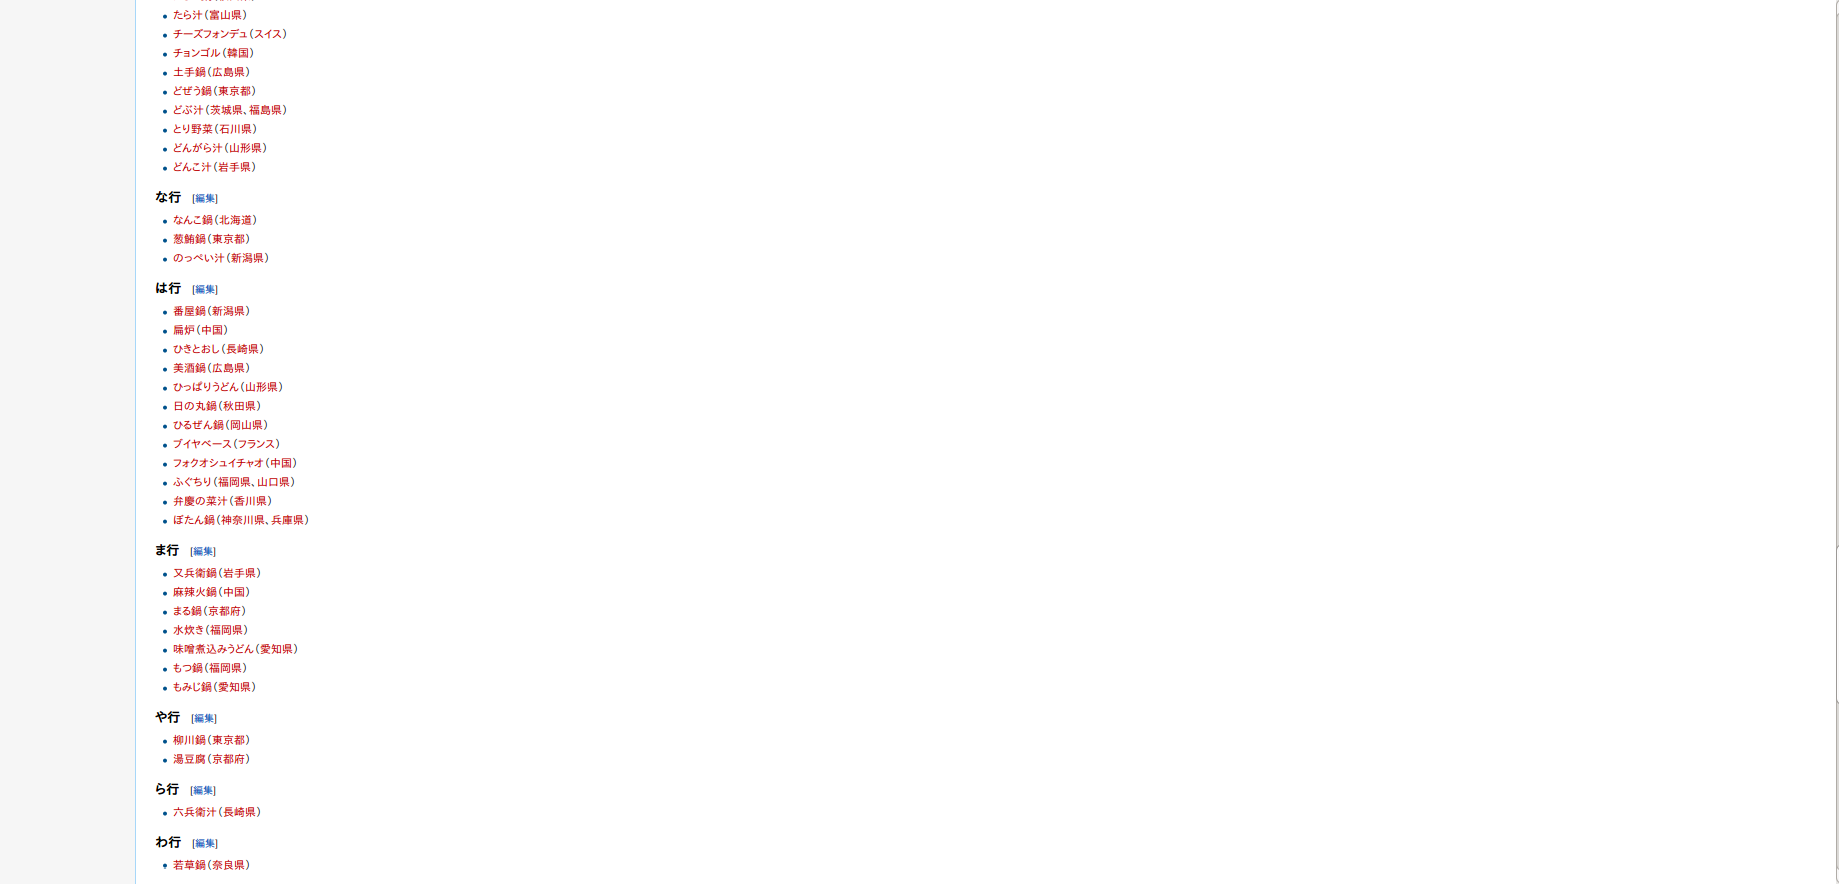
\includegraphics[width=18cm]{nabe4}
\caption{鍋料理画理4}\label{nabe4}
\end{figure}
\clearpage

\subsection{テスト}
ページを作成した後は,端末でコードを以下の通りに入力する.

3.MediaWikiの全データをXMLにダンプする.
{\small
\begin{verbatim}
php /var/www/html/mediawiki/maintenance/dumpBackup.php --current > all-pages.xml
\end{verbatim}}

圧縮して, all-pages.xml.bz2 を作る.
{\small
\begin{verbatim}
 bzip2 all-pages.xml 
\end{verbatim}}


ページを削除したい場合.
{\small
\begin{verbatim}
echo -e 'ハクサイ\n鍋料理' | php /var/www/html/mediawiki/maintenance/deleteBatch.php
\end{verbatim}}

XMLファイルのインポート.
{\small
\begin{verbatim}
bzip2 -dc all-pages.xml.bz2 | php /var/www/html/mediawiki/maintenance/importDump.phpの
\end{verbatim}}

ページの削除とXMLファイルのインポートを使えば,MediaWikiの内容を簡単に書き換えられる.

テストデータの解析
{\small
\begin{verbatim}
bash script/ex_hyponymy.sh -E -s -t ./data3 all-pages.xml.bz2
\end{verbatim}}

解析をすると解析結果は,ファイルのtmp \textbackslash ex-hyponymy-1,0のフォルダに出ている.解析結果は以下である.

\begin{figure}[!htb]
\centering
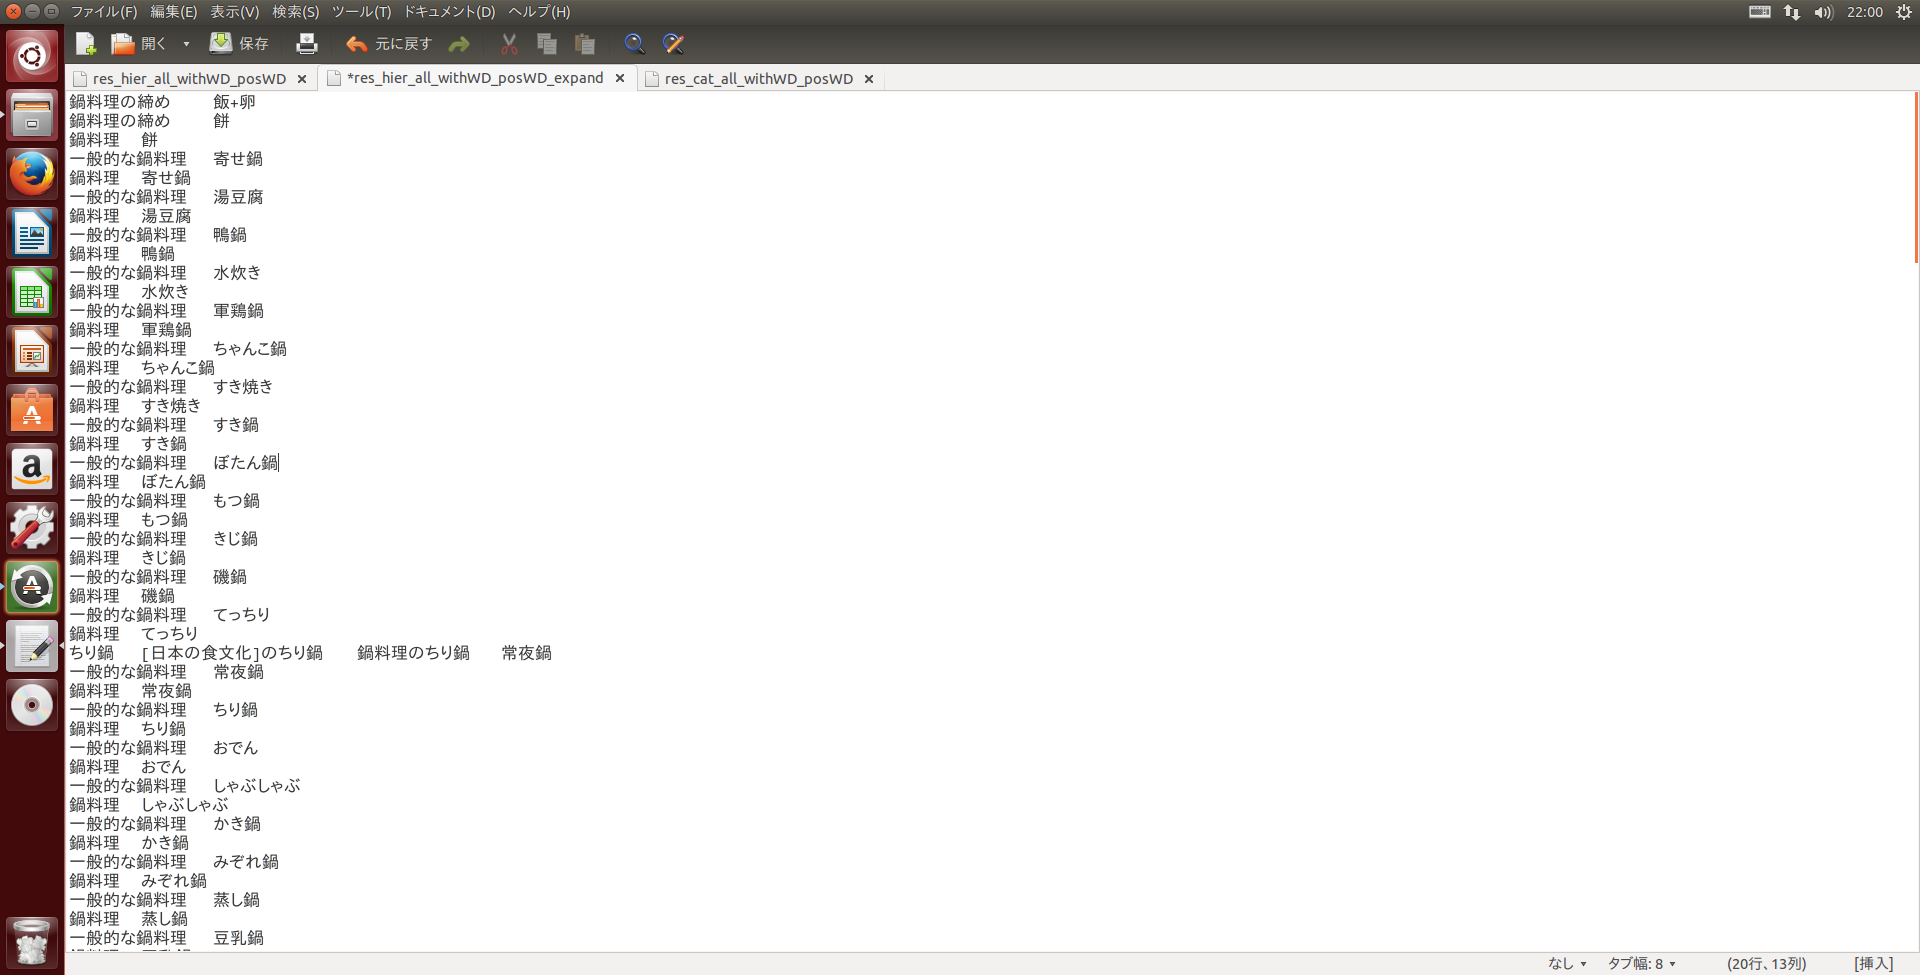
\includegraphics[width=18cm]{kaiseki1}
\caption{テスト解析結果1}\label{kaiseki1}
\end{figure}

\begin{figure}[!htb]
\centering
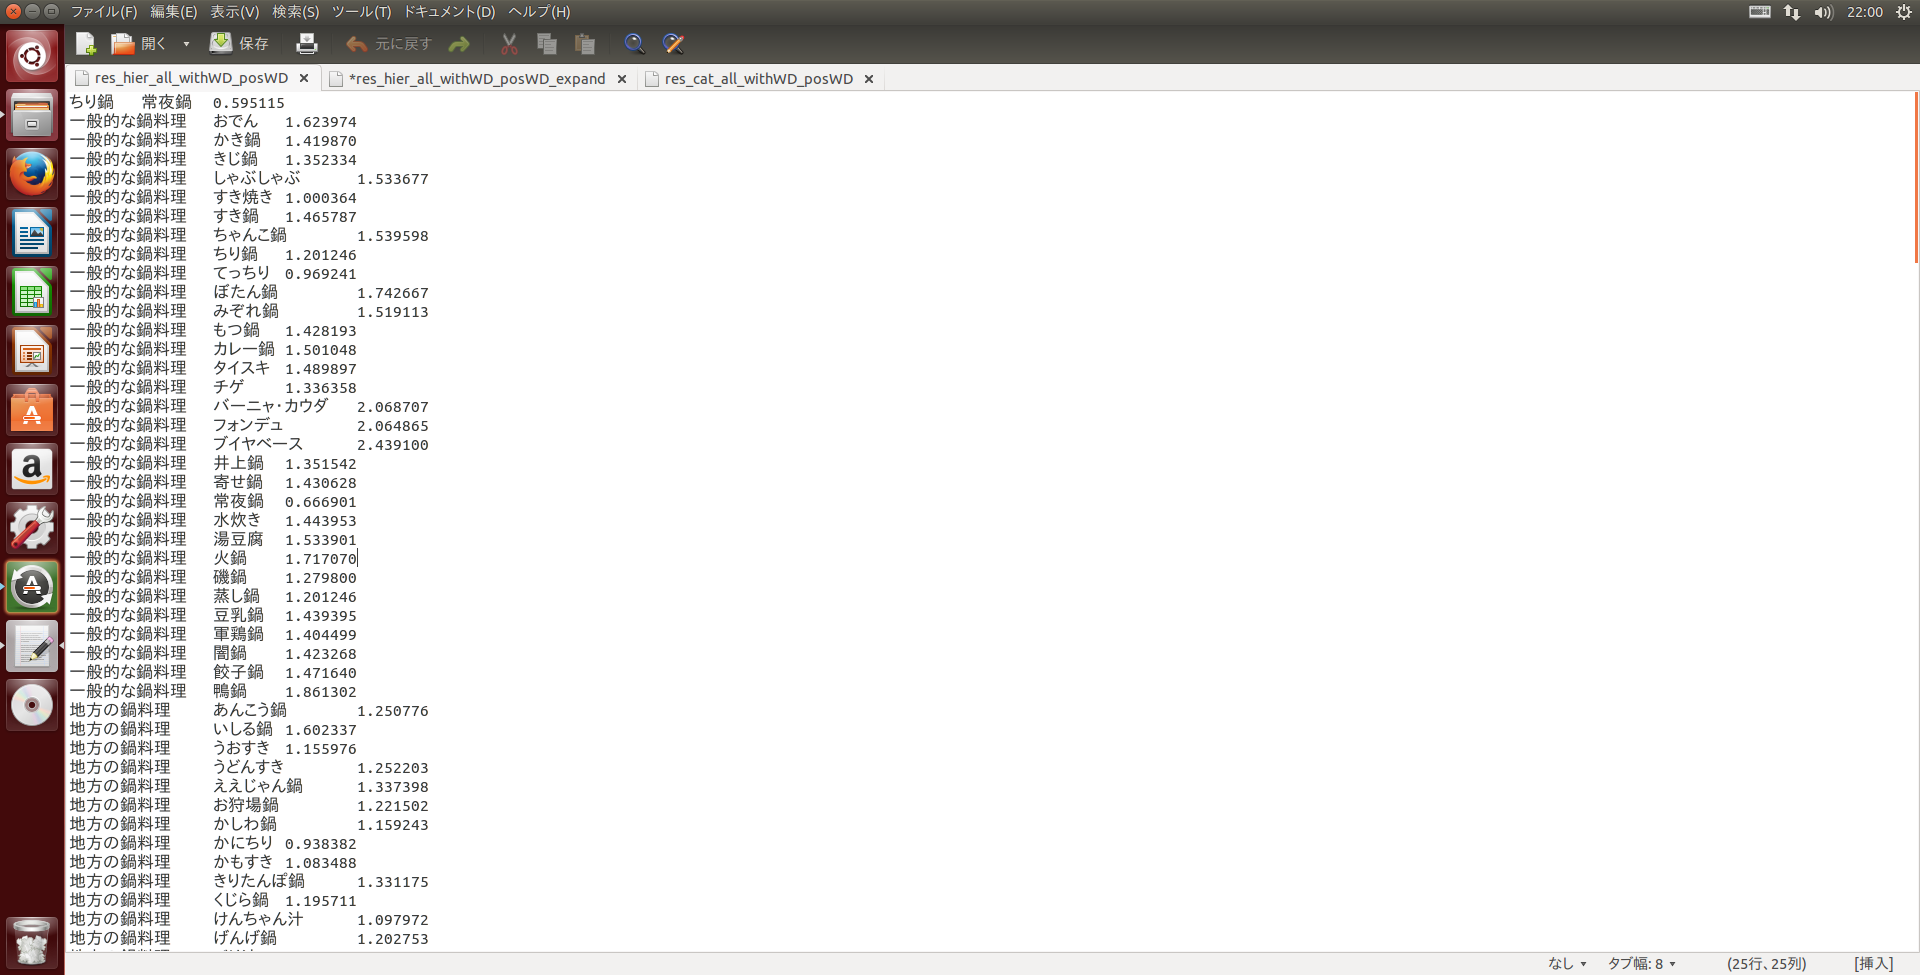
\includegraphics[width=18cm]{kaiseki2}
\caption{テスト解析結果2}\label{kaiseki2}
\end{figure}







\chapter{結果}
\section{本章の構成}
本章では,前章で記述した手法を用いた研究結果を記述する.



\section{研究結果}
Mediawikiとその解析結果を記述する.


\subsection{Mediawiki結果}
以下にMediawikiの結果を記述する.
\begin{figure}[!htb]
\centering
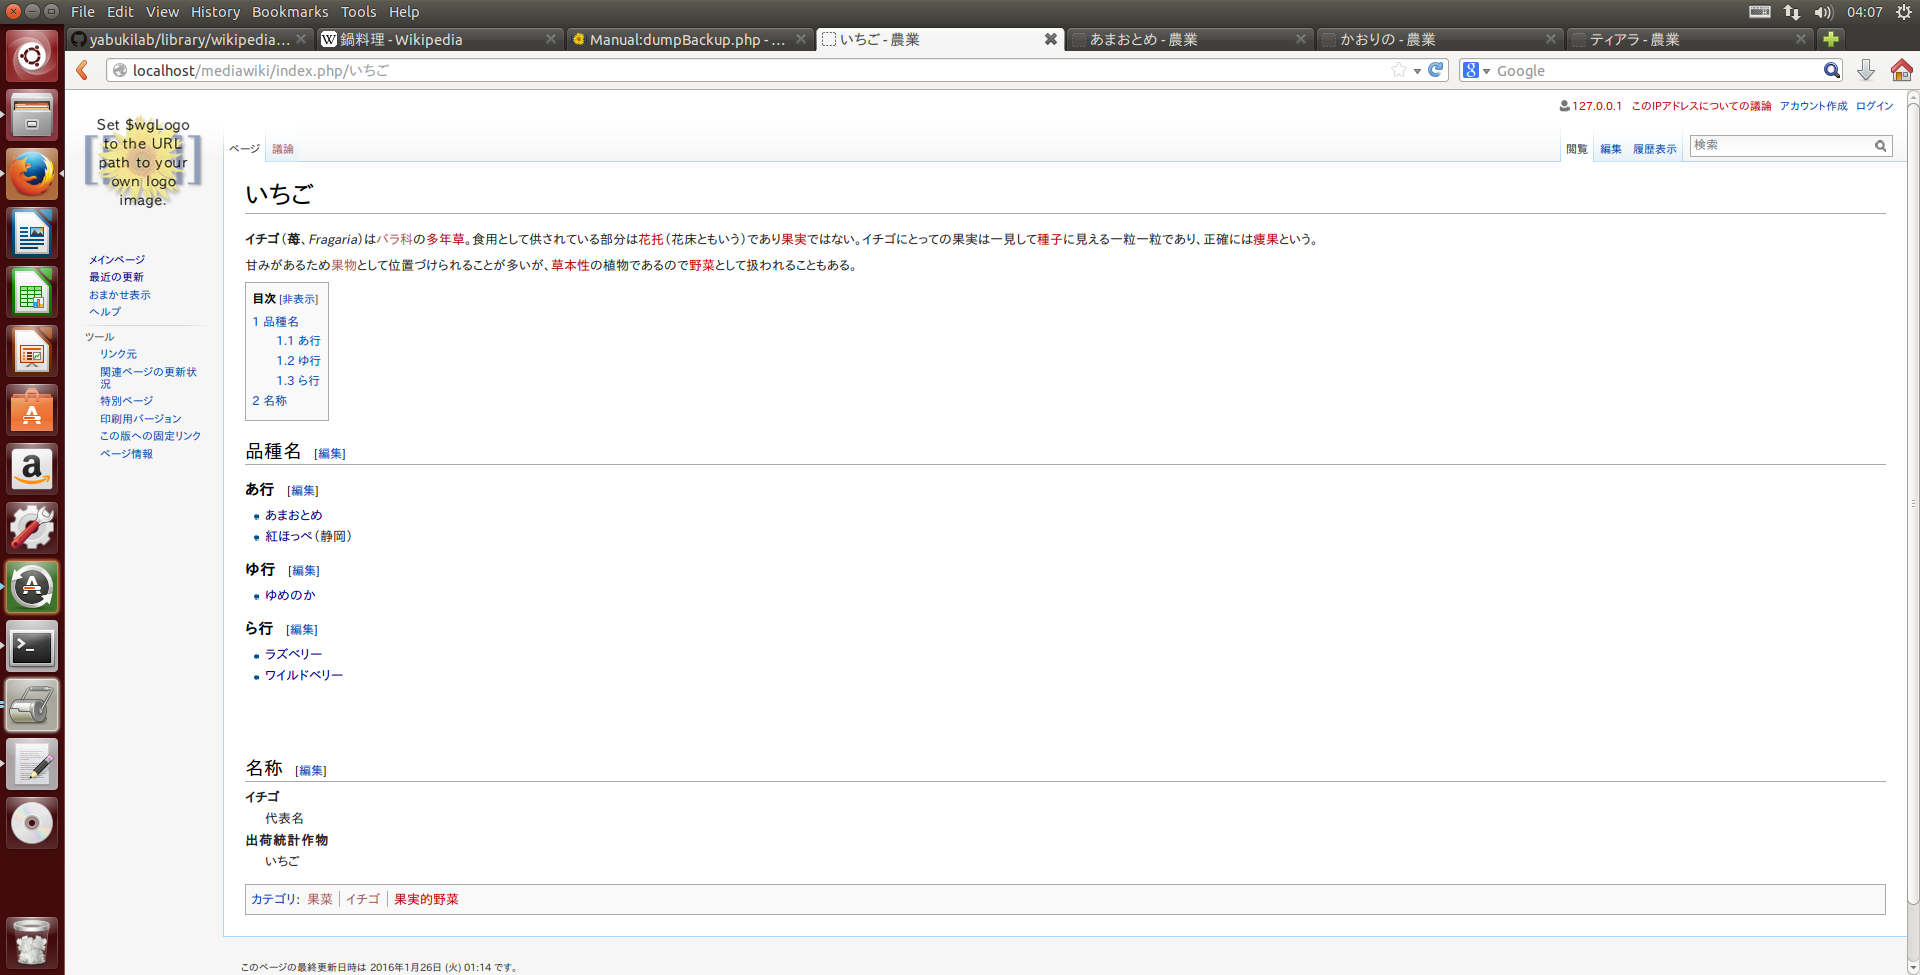
\includegraphics[width=18cm]{itigokekka.png}
\caption{Mediawiki結果}\label{itigokekka.png}
\end{figure}

\begin{figure}[!htb]
\centering
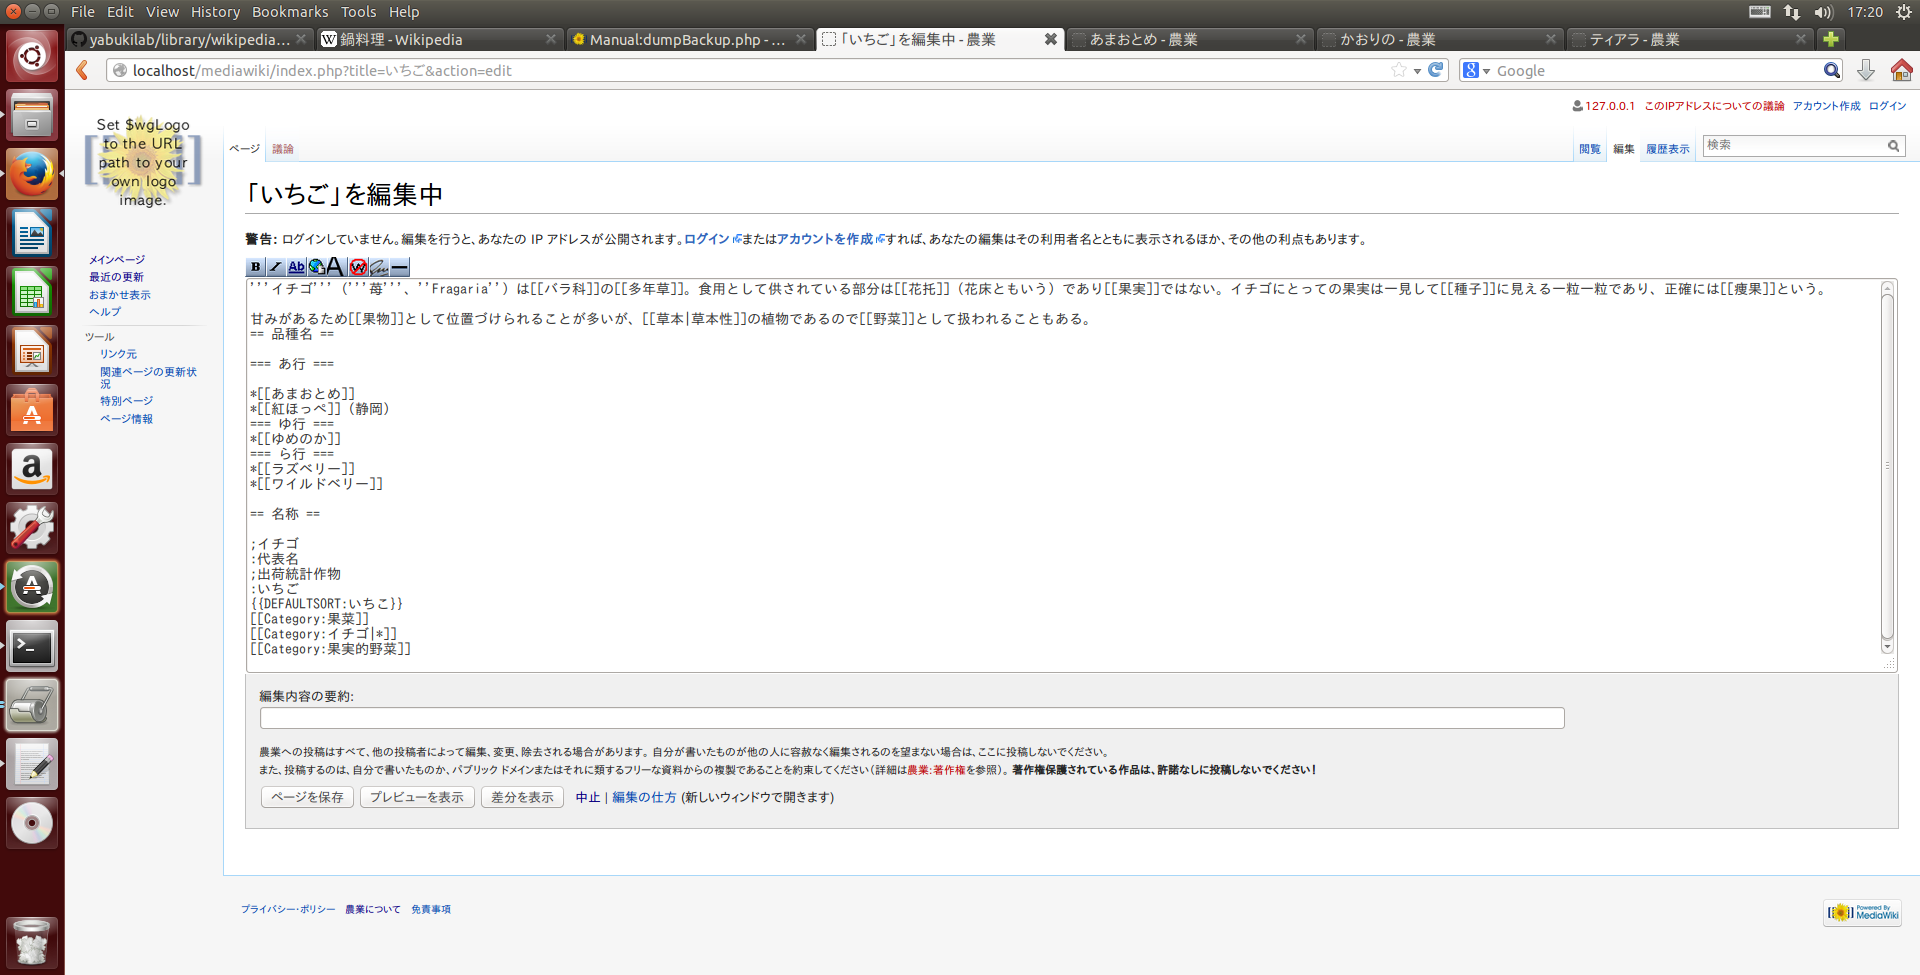
\includegraphics[width=18cm]{hensyuuseikou.png}
\caption{Mediawiki結果2}\label{hensyuuseikou.png}
\end{figure}


Mediawikiの構成は概要,品種名,名称,カテゴリにした.カテゴリは,種別の果菜,代表名のイチゴ,種類の果実的野菜にした.

\subsection{解析結果}
以下に解析結果を記述する.

\begin{figure}[!ht]
\centering
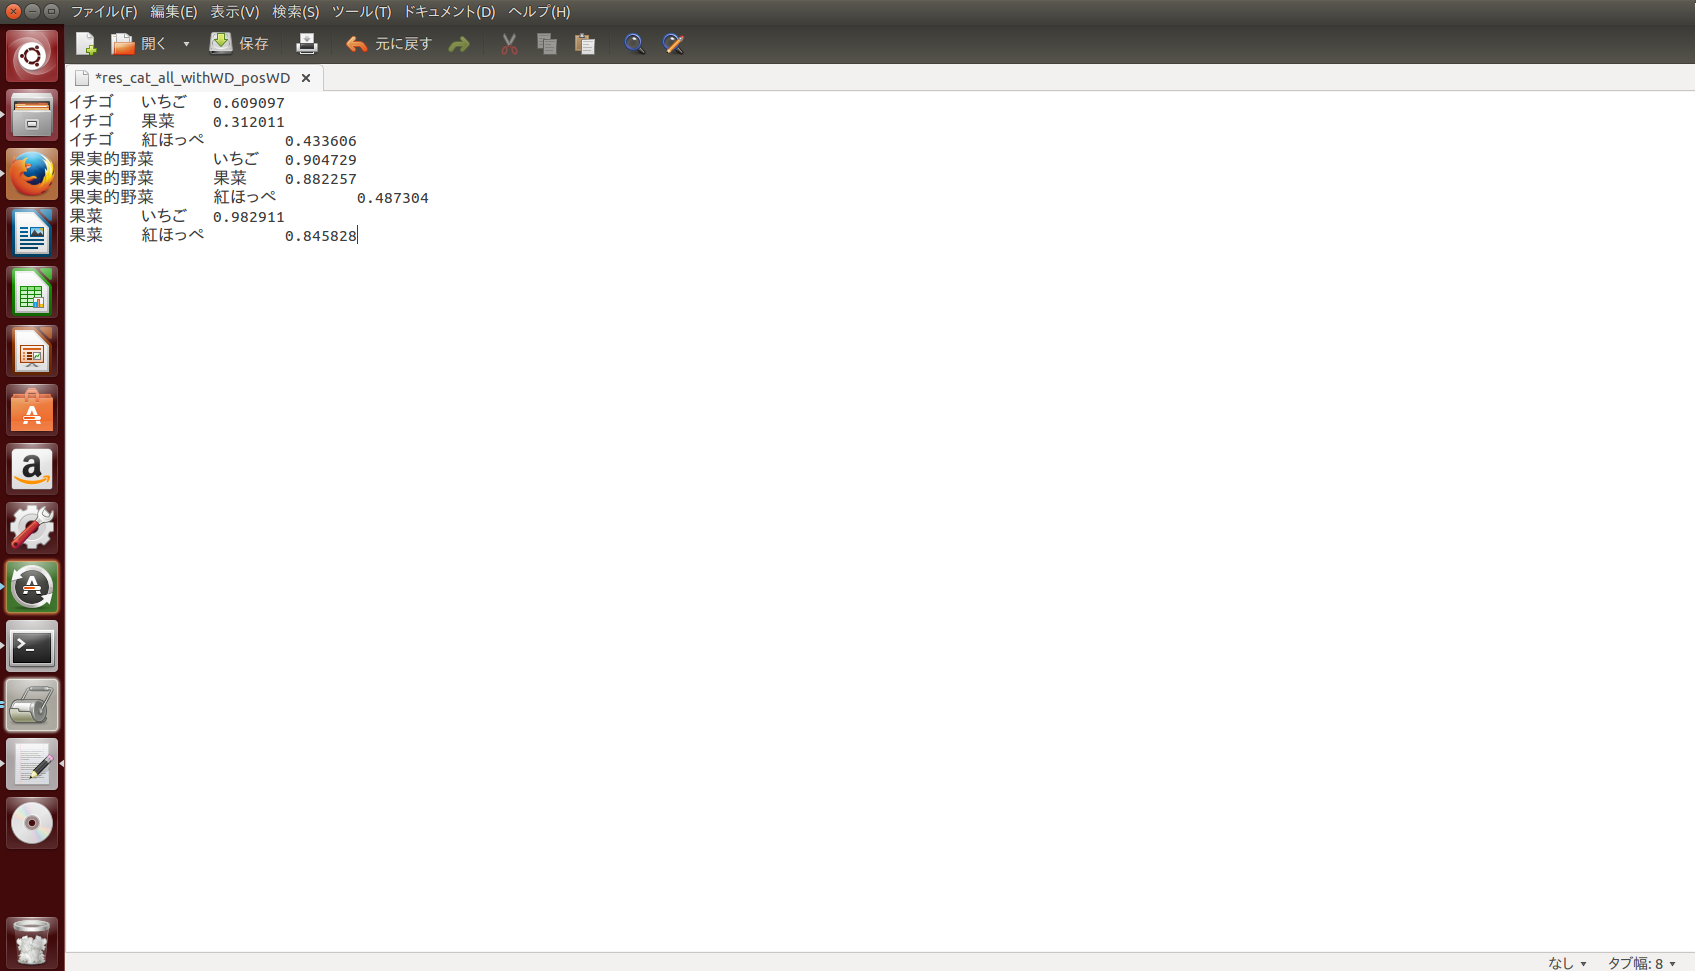
\includegraphics[width=18cm]{kekka}
\caption{解析結果1}\label{kekka}
\end{figure}



\begin{figure}[!htb]
\centering
\includegraphics[width=17cm]{kekka2}
\caption{解析結果2}\label{kekka2}
\end{figure}



\begin{figure}[!htb]
\centering
\includegraphics[width=18cm]{kekka3}
\caption{解析結果3}\label{kekka3}
\end{figure}

\clearpage

解析結果とMediawikiを比べるとカテゴリとページの作物名,品種と品種の名前,カテゴリと品種名に分けられている.最初の概要と名称の部分が解析されず,品種名とカテゴリは解析されている.

品種名は見出しのレベルを上げて書くことで解析されていると思われる.カテゴリは,書き込めば解析されることが分かった.そのため,カテゴリに代表名,種別,種類など書き込むことで図10.4のように目標のような解析結果になった.


\section{研究結果まとめ}
Mediawikiに様々な書き方をした解析することで成功するパターンを発見することに成功した.

Mediawikiの構成は概要,品種名,名称,カテゴリにした.カテゴリは,種別の果菜,代表名のイチゴ,種類の果実的野菜にした.そのうち解析されたのが品種名とカテゴリでカテゴリに代表名,種別,種類などを記載して,品種名の記事の見出しのレベルを上げて書くことで目標とする解析結果を表示できた.



\chapter{考察}
\section{本章の構成}
本章では,8章と9章で記述した本研究についての考察を記述する.

\section{考察}
本研究では,品種名とカテゴリのパターンを発見できた.品種名のパターンは,見出しのレベルを上げてレベル3の見出しを五十音順に並べることで容易に編集できると考えられる.なぜなら五十音順に並べることで,生産者は,農作物名を追加するだけだからである.

本研究でカテゴリは代表名,種別,種類などを記述したが,目的に応じた名称をカテゴリに記載することで目的に応じた翻訳をすることができるだろう.

さらに本研究では,農業だけでなく同じ意味を持ち,違う語彙を持つものの翻訳に使用することができるだろう.


\chapter{結論}
\section{本章の構成}
本章では,ここまでの本研究の結論を記述する.

\section{結論}
本研究は,様々な目的により語彙が変わる農作物を標準化できないかを考えた.しかし異なる企業や団体の意思を1つにまとめるのは,困難である.

そのため異なる作物名称を目的に応じた変換(翻訳)するための,共通する仕組みがないかということに着目した.用語の変換をするために用語を上位下位で結び,関連用語を抽出することを考えて翻訳できる仕組みを目的とした.

本研究では,Mediawikiに情報を書き込み,その情報を上位下位関係抽出ツールを用いて抽出して翻訳を試みた.その結果,カテゴリを登録して,見出しのレベルを上げて書き込むことで目標とする解析を達成することに成功した.

今後は,見出しのレベルを上げる以外のパターンを見つけ,より編集をしやすくすることが今後の課題であろう.



\bibliographystyle{junsrt}
\bibliography{biblio}%「biblio.bib」というファイルが必要.

\end{document}


